\documentclass[12pt,PhD]{muthesis}
\bibliographystyle{styles/vancouver}
\usepackage{cite}
\usepackage{graphics}
\usepackage{amstext}
\usepackage{amsmath}
\usepackage{algorithm}
\usepackage{algorithmic}
\usepackage{booktabs}
\usepackage{url} % typeset URL's reasonably
\usepackage{listings}

\newcommand{\unit}[2]{\ensuremath{#1\,\text{#2}}}
\newcommand{\cms}[1]{\ensuremath{#1\,\text{cms}^{\text{-1}}}}

\newcommand{\ms}[1]{\unit{#1}{ms}}
\newcommand{\msrange}[2]{\ensuremath{#1\text{--}#2\,\text{ms}}}
\newcommand{\mm}[1]{\unit{#1}{mm}}
\newcommand{\mv}[1]{\unit{#1}{mV}}
\newcommand{\degr}[1]{\ensuremath{#1^{\circ}}}

\newcommand{\supers}[1]{\ensuremath{^{#1}}}
\newcommand{\subs}[1]{\ensuremath{_{#1}}}
\newcommand{\ii}[1]{\ensuremath{\text{\emph{I}}_{\text{#1}}}}
\newcommand{\iip}[1]{\ensuremath{\text{\emph{I}}'_{\text{#1}}}}
\newcommand{\g}[1]{\ensuremath{\text{\emph{g}}_{\text{#1}}}}

\newcommand{\apd}[1][90]{APD\subs{#1}}
\newcommand{\apdr}[1][90]{APD\emph{r}{\scriptsize,#1}}


\newcommand{\nothree}{\ensuremath{\text{NO}_{3^{\text{-}}}}}

% picture predefines
\setlength{\unitlength}{1mm}

\newsavebox{\resistor}
\savebox{\resistor}(10,2)[bl]{
\put(0, 1){\line(1, 0){1}}
\put(1, 0){\line(0, 1){2}}
\put(1, 0){\line(1, 0){8}}
\put(1, 2){\line(1, 0){8}}
\put(9, 0){\line(0, 1){2}}
\put(9, 1){\line(1, 0){1}}
}

\newsavebox{\vresistor}
\savebox{\vresistor}(2, 10)[bl]{
\put(1, 0){\line(0, 1){1}}
\put(0, 1){\line(1, 0){2}}
\put(0, 1){\line(0, 1){8}}
\put(2, 1){\line(0, 1){8}}
\put(0, 9){\line(1, 0){2}}
\put(1, 9){\line(0, 1){1}}
}

\newsavebox{\cell}
\savebox{\cell}(10,10)[bl]{
\put(0, 0){\line(0, 1){10}}
\put(10, 0){\line(0, 1){10}}
\put(0, 0){\line(1, 0){10}}
\put(0, 10){\line(1, 0){10}}
}

% algorithmic package
\renewcommand{\algorithmiccomment}[1]{// #1}

\begin{document}

    \title{Developing Realistic Models of the Atrium and the P-Wave ECG}
    \author{Jonathan D. Stott}
    \principaladviser{Henggui Zhang}
    \school{School of Physics and Astronomy}

    \beforeabstract
    \prefacesection{Abstract}
    \singlespace
    The University of Manchester\\
Jonathan David Stott\\
Doctor of Philosophy\\
Developing Realistic Models of the Human Atrium and the P-Wave ECG\\
23rd September 2009\\

Cardiac disease, including atrial fibrillation (AF), is one of the biggest causes of
morbidity and mortality in the UK, accounting for one third of all
deaths.\cite{foo}
Cardiac modelling is now a well established field.
Mathematical models offer a valuable way of gaining insight into the dynamic
behaviours of the heart, in normal and pathological conditions.
Great efforts have been put into modelling the ventricles, whilst the atria have
received less focus.
This thesis therefore concentrates on developing models of the atria.

In the first part of the thesis, I developed a simulation toolkit for
modelling myocyte electrophysiology and excitation waves in 1D \& 2D
tissues.
It includes optimisations such as adaptive stimulus protocols.
As examples of application, it is used to investigate effects of a novel anion
bearing current on atrial excitation and the effect of AF remodelling on atrial
myocyte electrical heterogeneity.

In the second part, a computationally efficient and anatomically based model of
the atria is constructed.
The 3D model includes heterogeneous, biophysically detailed
electrophysiology and conduction anisotropy.
The full model activates in \ms{121}\ in sinus rhythm, in
close agreement with clinical data.
The model is used, with the toolkit, to investigate the function effects of S140G
mutation in KCNQ1 which is associated with familial AF.

In the last half of the thesis, the 3D model forms the core of a boundary
element model of the P-wave Body Surface Potential (BSP).
The BSP model incorporates representions of the lungs and the heart blood masses.
Generated ECGs show qualitative agreement with clinical data.
Their morphology is as expected for a healthy person, with a lead II duration of
\ms{103}.
The BSP model is used to verify an existing algorithm for focal atrial
tachycardia location and in providing explanation for a novel clinical
phenomena, inverted P-waves at night.


Models of the human atria and body surface potential are constructed.
The models are validated against both experimental and clinical data.
These models are suitable to use as the platform for further research.



    \onehalfspace
    \afterabstract
    \prefacesection{Acknowledgements}
I would like to thank my supervisor, Dr. Henggui Zhang of the Biological Physics
group at Manchester, for his support and guidance throughout my thesis.
Without his help, this work would not have been completed.

I would also like to thank all of the members of the Biological Physics group,
past and present, for their conversations on the thesis and on the topics around
it (and everything else).
Through them I have learned of papers I might have missed and considered avenues
of investigation that otherwise I might not have done.

Another debt of gratitude is owed to Doctors Clifford Garret, Derek Rowlands and
Gwilym Morris.
Their discussions about the ECG in general and the ones produced in this thesis
in specific were helpful as I refined the model.

My parents, David and Judith Stott and my sister, Joanna.
I'm not sure how to thank them for all their love and support as I have worked
on thesis.

My friends, both local and remote.
For occasional discussions about programming, my work and anything else that was
on my mind.
They've helped me, probably in more ways than they know.

Finally, I would like to thank all those who saw drafts of this thesis.
Without them, the final text would have more errors.
Though of course, any mistakes which remain are my own.


    \afterpreface
    

   \chapter{Introduction}

Cardiac disease is one of the biggest causes of death in the UK, causing over
one third of all deaths.
In addition to the deaths, many more people suffer the after effects of a heart
attack or live with the difficulties caused by heart failure~\cite{bhf2008}.
These figures are duplicated across much of the developed world.

Mathematical modelling of the heart offers a way of gaining insight into the
cardiac processes and the mechanisms of cardiac disease.
It is a well established field of research with numerous international journals
and conferences discussing the findings.
Mathematical models allow physiological effects to be dissected and quantified
in ways that can be difficult for in vivo and in vitro experiments.
This can be used to inform both further experiments and clinical diagnosis and
treatment.

Mathematical models exist for many different types of cardiac cells and
cardiac tissue.
Many studies of cardiac tissue focus on the ventricles, with atrial studies less
common.
This is in part because failure of the ventricles can have a much more serious
impact, but in spite of this, the atria represent an interesting target to
study.
They have a complex electrophysiology and topology.

This study therefore aims to construct a series of models and tools for studying
the atria of the heart.
This involves modelling the atria and their processes on a wide variety of scales,
from the single cell to the whole atrium.
To enhance the clinical relevance of the study, a model of the atrium sitting
within the human torso will also be constructed.
This will allow the P-wave ECG to be calculated, the first view many cardiac
physicians will have of a failing atrium.
The tools will then be used to study a variety of factors that influence atrial
behaviour.


\section{The Heart}

The heart's role is to pump blood around the body, driving in the circulation of
the blood and everything contained within it.  It is one of the most important
organs in the body and any malfunction in its behaviour could be fatal in very
short order.  It begins beating in the early stages of pregnancy and continues
until death, hopefully many decades later.  It beats at an average rate of
around 70 beats per minute (bpm) for the adult male and 75 bpm for the adult
female.

The heart is not, as popular belief would have it, the seat of human emotion.
The functioning of the heart is modulated by such emotion however, slowing when
we are calm and increasing in rate quite dramatically when we are excited or
afraid.  Despite being influenced by the brain and our emotional states, the
heart drives itself, rather than having the pace-making initiated outside the
organ.

\subsection{Location of the Heart}

The human heart sits in the centre of the chest, the bulk of it extending into the
left-hand side of the chest cavity, inside a fibrous sac called the pericardium.
The actual location, orientation and size can vary quite significantly from
individual to individual~\cite{Oberman1967}.


\subsection{Gross Structure of the Heart}

The heart is mostly muscle.
This muscle is anchored to a collagenous `skeleton', known as the annulus
fibrosus located at the atrio-ventricular junction.
The muscle is different from the `smooth' skeletal muscle, in both structure
and behaviour~\cite{Katz2006}.

The human heart has four chambers, two atria and two ventricles.  The atria receive
the blood from the circulatory system and force it into the two ventricles,
which then contract and force this blood out and around the lungs and body.
These chambers are known as the left and right atria and the left and right
ventricles.  The left hand side of the heart in humans is much more developed
than the right.
This is due to their differing roles in circulating the blood.

The right and left atria are smaller than their respective ventricles and have
much thinner walls, because they need to develop much less pressure.  The right
atrium receives the blood from the circulatory system which is de-oxygenated,
and passes it on to the right ventricle.  The left atrium receives the highly
oxygenated blood from the lungs, and passes it onto the left ventricle.  The two
atria are separated by a thin muscle wall known as the intra-atrial septum.
This prevents the mixing of blood between the two atrial chambers.

The differences between the right and left ventricles are much more pronounced
than those between the right and left atria.  The right ventricle must merely
pump blood around the lungs and developing too high a pressure there could
actually damage the delicate structures.  By contrast the left ventricle must
develop enough pressure to drive blood around the whole body and as such it is
much more muscled.  Again, the two ventricles are divided by the ventricular
septum.

As noted earlier, separating the atria and ventricles is the annulus fibrosus
or central fibrous body.
This is a dense layer of fibrous tissue.
In addition to providing an anchor for the muscle of the heart, it electrically
isolates the atria from the ventricles.
In the normal heart, the only electrical connection between the atria and the
ventricles is at the atrio-ventricular node.
This connects the right atrium to the specialist conduction system of the
ventricles.

\subsection{The Atria}

Examination of the human atria (or auricles, in older literature) is as old as studies
of the heart.
However, in recent years there has been a renewed interest in the
atria and their structures.
This has followed an increasing appreciation that the atria are not merely
reservoirs of venous blood, but have an active role to play in the function of
the heart~\cite{Ho2002a,Ho2002b,Ho2009,Platonov2007,Platonov2008a}.

Descriptions of location of features use the `altitudinal' description, where
this is possible.
Altitudinal descriptions use the coordinates of the body, such that `right' is
the body's right hand side, not the right of the observer.
In this description, the atria are located to the right of the ventricles.
They can be slightly superior, too.
The right atrium is anterior and to the right, the left atrium more posterior and to
the left of the body.

The atria have a number of common features.
Both have a valve on the base, which is part of the central fibrous body.
In the right atrium, this is the tricuspid valve, in the left, the mitral valve.
These valves feed into the respective ventricles.

Both atria also have appendages, although the appendages differ in form.
The right atrial appendage is large, with a triangular shape and a wide base.
It is located anteriorly and superiorly on the right atrium.
By contrast, the left atrial appendage is smaller and more tubular in nature.
It is located posteriorly and superiorly compared to the left atrium.

\subsubsection{The Right Atrium}

The right atrium gathers in blood from the body, after it has cycled around the
organs.
The right atrium has a simpler topology than the left atrium.
At the top is an opening for the superior vena cava, and at the base there are
openings for the inferior vena cava and the tricuspid valve.

The right atrium is the location of many of the important sites of the
conduction system of the heart.
The sinus node, or sino-atrial node (SAN), is located on the right atrial wall,
close to the superior vena cava.
The SAN is the primary pacemaker for the heart in normal function.
It achieves this through specialised cells, known as nodal cells.
These cells are what are termed `auto-active' and are capable of spontaneously
exciting.

Running down the lateral wall is a muscle ridge, known as the crista terminalis,
or terminal crest.
The crista terminalis delineates the smooth and rough parts of the right atrial
wall.
This muscle ridge consists mostly of myocytes arranged longitudinally along the
main axis of the ridge, and so forms a path of preferential conduction.
In addition, these cells have a specialised electrophysiology~\cite{Feng1998}.

At the inferior end of the crista terminalis there is the atrio-ventricular
node (AVN).
This is another area of specialised nodal cells.
These cells are also auto-active, although with a slower natural frequency than
the SAN.
They therefore only take over in the case of SAN failure.
The AVN is the only point of electrical contact between the atrium and
ventricles in the normal heart.
As well as providing a link between the atria and ventricles this region acts
to limit the rate of stimulus which is passed on to the ventricles, protecting
them from excessive atrial pacing rates.

Branching from the crista terminalis and spreading around the muscle wall of the
right atrium are the pectinate muscles.
Like the crista terminalis, these bundles consist mostly of cells lying end to
end, forming pathways of preferential conduction.
The conformation of the pectinate muscles varies between individuals; some have
complex branching and interwoven patterns, whilst others have simpler and
relatively parallel bundles.

\subsubsection{The Atrial Septum}

The atrial septum divides the two atria.
Much of the septum is actually an in folding of the right atrium.
The true septum is limited to the fossa ovalis and the muscle ring immediately
surrounding it.
The fossa ovalis is a valve which is important in fetal circulation, but is
closed in the normal adult.
The fossa ovalis is mostly fibrous in nature.
The muscle fibres run in a predominately circular direction around the fossa.

\subsubsection{The Left Atrium}

The left atrium gathers blood from the lungs.
The pulmonary veins tend to give the left atrium a more complex topology than
the right.
This complex topology can make the pulmonary veins a source of arrhythmic
activity.

Unlike the right atrium, the left atrium is not dominated by the appendage.
In the left atrium, the appendage is small and largely separate from the main
body of the atrium.
The endocardial surface of the appendage is covered in many fine muscle ridges.
Between these ridges, the walls of the atrium can be paper thin.

Conventionally the left atrium is depicted as having four openings for the
pulmonary veins.
Recent studies suggest considerably more variation with approximately one third
of hearts having merged veins on one or both sides.
In some cases, the single vein can actually link all the way to the lungs.
The pulmonary veins are surrounded by a sheath of tissue.
There is evidence that cells in the sheaths can have different electrophysiology
to normal atrial cells~\cite{Jones2008}.

The left atrial wall has relatively smooth walls.
However, it is not uniform in thickness or muscle architecture.
It instead has a complex and overlapping muscle structure.
This can look like layers, but there are no insulating fibrous sheets between
bundles.

\subsubsection{Inter-atrial Connections}

The atria are linked by muscle bundles.
These muscle bundles have cells mainly oriented end to end, which gives
preferential conduction along their axis.
The most well known of these is the Bachmann's bundle, which is located
anteriorly and superiorly between the two atria.

Common thought has it that the Bachmann's bundle is the principle electrical
connection between the atria in sinus rhythm.
However, recent studies (summarised in~\cite{Platonov2007,Platonov2008a}) have
found that in a significant fraction of the population, a secondary pathway
which is inferior and/or posterior is used instead.
In some subjects, a Bachmann's bundle cannot even be located.
There is a lack of studies performed on healthy subjects, however, so it is
unclear on what occurs in the normal case.

\subsection{Cardiac Myocytes}

Myocytes, or muscle cells, comprise the vast bulk of cardiac tissue.
They both conduct signals and contract to provide the force needed to pump the
blood around the body.
This is accomplished by a complex interplay of ionic
currents~\cite{Katz2006}.

\subsubsection{Myocyte Structure}

A typical human myocyte is from 50 to 150$\,\mu$m long, and has a radius
between 10 and 20$\,\mu$m.
They have a roughly cylindrical shape.
The cell is wrapped in an impermeable membrane, called the sarcolemma or plasma
membrane.
The membrane in many myocytes is invaginated at various points by series of
fine transverse tubules (T tubules) that carry action potentials deep into the
myocytes.

The cellular membrane contains a large number of specialised structures
responsible for allowing a regulated flow of ions into and out of the cell.
These structures include passive channels, active pumps and gated channels.
They are used to modulate the ionic composition of the intracellular
space and play a vital role in modulating the electrical activity of the cell.
Because it is impermeable a potential difference can build across the membrane,
between the inside and outside of a cell.
This is known as the membrane potential.

Within the cells, much of the space is filled with what are called
myofibril-like units, long branching fibres about 1$\mu$m in diameter.
These fibres are divided up into scarcomeres, approximately 2$\mu$m long in the
resting myocyte and is considered the basic contractile unit.
Mitochondria, which provide the ATP needed to provide energy for the
contractions, also occupy a significant fraction of the intracellular space.
Mitochondria are not actually a part of the body in the strictest sense and
have their own DNA -- they are symbiotic organisms that entered our own cells
at some unknown time in the past.
One other structure within the cells that is important to the electrical and
mechanical behaviour of the cells is a second tubule network, known as the
sarcoplasmic reticulum (SR) and the sarcotubular network.
The SR stores calcium in subsarcolemmal cisternae, which is released during the
membrane depolarisation.
The cisternae form structures known as dyads (or diads) with the T tubules.

\subsubsection{Ion Channels and Pumps}

The structures in the cellular membrane which permit ion channels to cross can
be roughly divided into channels and pumps.
Most channels and pumps are specific to one specific ion type.
Channels passively allow ions to flow with the concentration gradient, whilst
pumps actively move ions, regardless of the gradient~\cite{Hille2001}.

Channels and pumps are classified by the ion(s) they transport and how they are
controlled.
They are also classified on the direction of charge flow.
An inward current is one that would have the effect of a positive ion entering
the cell and could therefore also be caused by negatively charged ions exiting
the cell.
Inward currents act to increase the potential in the cell.
Conversely, outward currents are those that would have the effect of a positive
ion leaving the cell.
They are repolarizing currents as they act to decrease the membrane potential.

Inter-cardiac current flows through the gap junctions, which allow for large
current flows.
These are formed at the centre of membrane structures known as intercalated
disks.
The intercalated disks are concentrated at the ends of cells, although there are
some transverse connections.

Channels rely on an ionic gradient to drive flow through them.
Some channels have a constant conductance.
These are typically called background currents.
Channels with a conductance which depend on the instantaneous membrane potential
are known as voltage-gated channels.
Other channels can have their conductance modulated by the presence of a
hormone or chemical, such as the ATP sensitive potassium channel.

\begin{figure}
\begin{center}
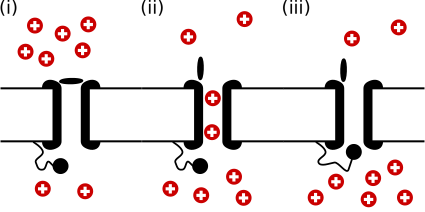
\includegraphics{figures/intro/activation_gate}
\end{center}
\caption[Time-Dependent Ion Channel]{
\label{fig:intro:heart:gated_ion}
A time dependant ion channel, represented by the black structure which bisects
the membrane (horizontal lines) for positive ions, shown as red circles.
The channel has an activation gate, the black lozenge on the top of the
membrane and an inactivation gate, the ball and chain on the underside of the
membrane.
In panel (i) the gate is not activated and shows a large concentration of ions
on the upper side.
In panel (ii), the gate activates and ions flow down the channel to the region
of lower concentration.
In panel (iii), the inactivation gate has moved to close the channel and no more
ions flow.
}
\end{figure}


Many gated channels are what are known as time-dependent channels.
These channels have structures over one or both ends which modulate the total
conductance to open (activate) or close (inactivate) the channel.
This is illustrated in figure~\ref{fig:intro:heart:gated_ion}.
The time course of this activation or inactivation is normally modulated by the
voltage, but can also be modulated by ion concentration or other mechanisms.

\begin{figure}
\begin{center}
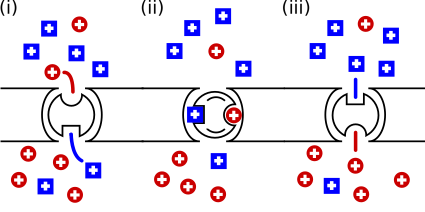
\includegraphics{figures/intro/ion_pump}
\end{center}
\caption[Ion Pump]{
\label{fig:intro:heart:ion_pump}
An ion pump (or more accurately, an ion exchanger), represented by the black
structure which bisects the membrane (horizontal lines) for two species of
positive ion, represented by red circles and blue squares.
The pump works against the concentration gradient.
In panel (i), the two ions bind to their respective sites on the pump.
In panel (ii), the pump changes its structure, drawing each ion through the
membrane.
In panel (iii), the pump releases the binding of the ions, letting them rejoin
the free ion populations.
}
\end{figure}

Pumps use energy to actively move ions against the gradient.
Complex molecules latch onto the ions on one side of the membrane and move them
through to the other side.
Many pumps are actually exchangers, which take in ions of one sort on one side
whilst transporting another type of ion the other way.

\subsubsection{Myocyte Electrical Action Potentials}

The evolution of the electrical state of the cell, from polarised to depolarised
and back again is termed the action potential (AP).
The shape and duration of
the action potential is mostly determined by the channels, carriers and pumps
across the cellular membrane, though the internal and external concentrations of
several ions and molecules can also have a significant effect.
There are three
principle ion species involved in the development of the action potential;
sodium ($\text{Na}^{\text{+}}$), potassium ($\text{K}^{\text{+}}$) and calcium
($\text{Ca}^{\text{2+}}$).
The third, calcium, is also important for contractile function.
Chlorine ($\text{Cl}^{\text{-}}$) is also of importance in some cells.

\begin{figure}
\begin{center}
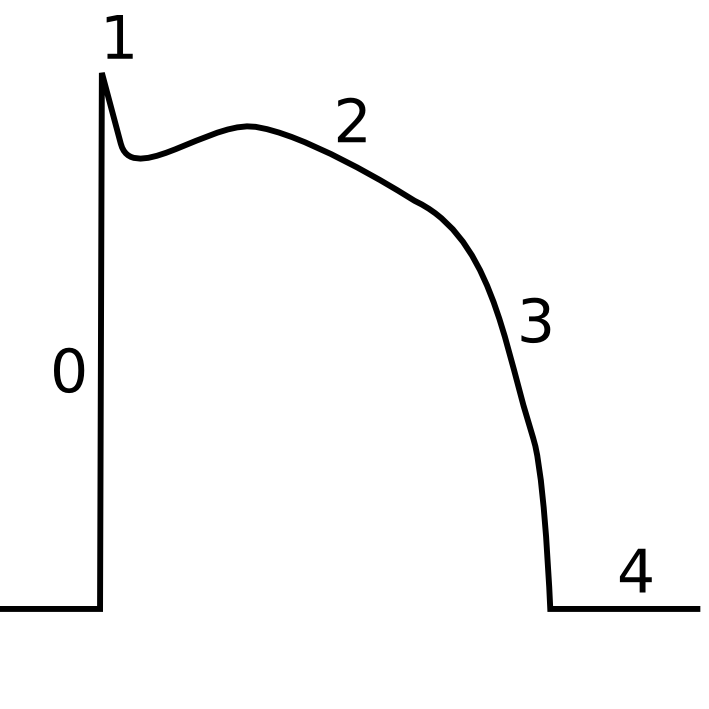
\includegraphics{figures/intro/ap_profile}
\end{center}
\caption[Schematic AP Profile]{
\label{fig:intro:heart:ap}
A schematic AP profile.
Labelled are the five phases of the action potential.
Phase 0, the upstroke.
Phase 1, the end of the upstroke.
Phase 2, the plateau.
Phase 3, the repolarization.
Phase 4, the resting period.
}
\end{figure}

The action potential has 5 phases (figure~\ref{fig:intro:heart:ap}).
It begins with depolarization, phase 0.
During depolarisation, the current is carried principally by the fast inward
sodium current.
Phase 0 is also known as the upstroke of the action potential, and its slope is
important to the propagation of the action potential through cardiac tissue and
also the excitability of the myocyte as in individual cell.
Phase 0 is over almost instantaneously in healthy myocytes.

Phase 1 signifies the end of the upstroke, and is caused by the inactivation of
the sodium channels.
The small notch present in some cellular action potentials is caused by a
transient net outward current, carried principally by potassium.

Phase 2 is the plateau phase.  This relatively long phase ($>$100ms in some
myocytes) is due to the balance of slowly activating inward calcium currents and
the outward potassium currents.
The inward calcium current is principally carried by the L-type calcium channels
and the outward potassium current by a plethora of channels, classified by the
speed of activation or the substance which modulates them.

Phase 3 is the repolarization period.
The calcium channels have inactivated.
The potassium currents are still open, and the net efflux of positive charge
repolarizes the cell.

The final phase 4 is the period during which the cell is at the resting
potential.
In addition, for a short period of phase 4, the cell is in fact
impossible to excite above this resting potential due to the inactivations of
numerous channels.
This is called the refractory period.

Both the shape and the length of the action potential have physiological
importance.
Many pathological conditions have a significant impact upon both.
The action potential duration (APD) is often given as an \apd\ or
\apd[50], denoting the duration of the AP at 90\% or 50\% repolarization,
respectively.

\section{Mathematical Models of the Heart}

Cardiac tissue has been modelled mathematically for about fifty years.
While initial models were simple, there are now models of high sophistication
available.
These models are capable of reproducing both healthy and pathological behaviour
with some accuracy.

\subsection{Categorising Myocyte Models}

Cellular models tend to be classified in two ways.
The first differentiator is the level of detail employed.
The second is on which cellular processes are modelled.

Biophysically detailed models are complex.
They consider the interactions of several different currents, and potentially
intra- and extracellular ion concentrations, reservoirs as well as other
details.
The second type are simplified, phenomenological, models.
These do not consider individual ion concentrations but instead just reproduce
one desired factor, typically the action potential profile.

Models, whether biophysically detailed or not, can concern themselves with the
cellular electrophysiology, the mechanical contrations or both.
This thesis concerns itself just with electrophysiological models.
Models of the mechanics are not considered and are not treated in this
description of mathematical modelling.

\subsection{A Brief History Of Cardiac Myocyte Modeling}

The first model of cardiac electrophysiology was published by
Noble~\cite{Noble1962}, and modelled Purkinje fibre (A specialised part of the
ventricular conduction system) action potentials.
Shortly thereafter, various refinements were published, as further experimental
data became available.
This was eventually followed by the Beeler--Reuter~\cite{Beeler1977}\ model of
the guinea pig ventricular myocyte.

The Luo--Rudy guinea pig ventricular myocyte model was first published in
1991~\cite{Luo1991} and was then sub-sequentially majorly revised and
republished in 1994~\cite{Luo1994}.
The first Luo-Rudy model was based on the Beeler--Reuter model, though with updated channel behaviours
and more complex potassium channels.
The second Luo-Rudy model was the first of the `second generation' models,
with fluctuations in all ion concentrations, and a much more detailed series of
equations for calcium handling.

In 1998, the Courtemanche--Ramirez--Natel\cite{CRN98}\ (CRN) model and the
Nygren~\cite{Nygren1998}\ model were published.
These were both models of the human atrium.
They were also both second generation models, with detailed calcium handling.
Also in 1998 Fenton and Karma published their phenomenological
Fenton--Karma~\cite{Fenton1998}\ model, which used just three channels to
reproduce the shape of the ventricular action potential.

\subsection{Mathematical Models of Myocytes}

Mathematical models of cardiac myocytes are built from a few simple assumptions
and considerations.
These concern the behaviour of the cellular membrane and ion channels.
The important ones are detailed here.

\subsubsection{Electric Circuit Model}

The electrical circuit model of the cell membrane underpins much of the work in
modelling the behaviour of cardiac myocytes.
It is however a very simple concept.
Since the membrane seperates charges, it may be considered as a capacitor, as
shown in figure~\ref{fig:intro:math:circuit}.
Since there is no net buildup of
charge on either side of the membrane, any ionic current, \ii{ion}, must be
countered by a capacitive current, and so
\begin{equation}
C_{m}\frac{dV_{m}}{dt} + \ii{ion} = 0
\label{eqn:intro:math:basic}
\end{equation}
where $V_{m}$ is the membrane voltage, and is defined as the difference between
the internal potential, $u_{i}$ and the external potential, $u_{e}$ or
\begin{equation}
V_{m} = u_{i} - u_{e}
\label{eqn:intro:math:vm}
\end{equation}
When multiple currents are considered, the total inward and outward currents are
summed.
The difficulty comes in determining the form of \ii{ion}, which varies widely
depending on the nature of the channel or pump in question.

\subsubsection{The Nernst Equilibrium Potential}

The Nernst equation is an important equation in electrophysiology.
It describes how the difference in ion concentrations on two sides of a
semi-permeable barrier can result in a potential difference across the barrier.
Any voltage dependant factor of a current of an ion, S, includes a reversal
potential, V$_{S}$, equal to the Nernst potential.
At the reversal potential, the current falls to 0.
When equilibrium is reached the potential difference, $V_{S}$, across the
membrane is given by
\begin{equation}
V_{S} = \frac{RT}{zF}ln\left( \frac{[S]_{e}}{[S]_{i}} \right) 
\end{equation} 
where subscripts $i$ and $e$ denote internal and external concentrations of S,
$R$ is the universal gas constant, $T$ is the absolute temperature, $F$ is
Faraday's constant and $z$ the charge of the ion $S$.

The Nerst Potential applies only to a single ion concentration.
This is not as large a limitation as it first might seem.
Whilst the action potential involves many ion species, many channels are ion
specific and thus the Nerst potential applies across them.

\subsubsection{The Hodgkin-Huxley Equations}

Many mathematical models of cardiac myocytes feature one or more
`Hodgkin--Huxley' channels.
Hodgkin and Huxley developed them in a now classic series of papers concerning
the current flow through the membrane of the squid giant axon.
They characterise the current flow with elegance and surprising accuracy.
It is important to note that the Hodgkin--Huxley equations consider the bulk
behaviour of the many thousands of individual channel structures distributed
across the membrane, not the behaviour of one single channel.

Hodgkin and Huxley started with a very simple assumption.
The current flow through a channel on the membrane, $I_{S}$ is given by
\begin{equation}
I_{S} = g_{S}\left(V-V_{S}\right)
\label{eqn:intro:math:hh1}
\end{equation}
where $g_{S}$ is the channel conductance, $V$ the membrane potential and $V_{S}$
the Nernst potential for the ion S.
Equation (\ref{eqn:intro:math:hh1}) assumes that the channel is selective for
one ion species S, and that the current is a simple linear function of the
voltage across the membrane.

With this underlying assumption, Hodgkin and Huxley set out to accurately map
the behaviour of the current with regards time and voltage.
The following section explains the description for the sodium current, \ii{Na}.
From the form of the sodium channel under voltage clamp conditions, it is
reasonable to expect $g_{Na}$ obeys a differential equation of the form
\begin{equation}
\frac{dg_{Na}}{dt} = f\left(v,t\right)
\label{eqn:intro:math:hh2}
\end{equation}
where $v=V-V_{Na}$.
However, the form of $g_{Na}$ is complex.
While remaining at the same voltage, the conductance at first increases and then
tails off.
It appeared that there were two processes at work, one that turned the current
on, and one that turned it off.
Hodgkin and Huxley realised that it would be easier to write $g_{Na}$ as a
function of two different variables.
One which corresponded to the turning on and one to the turning off of the
channel.
This leads there being an activation variable, called $m$, an inactivation
variable, called $h$ and that the current would be some linear combination of the
two, multiplied by a constant conductance factor $\bar{g}_{Na}$.
The two variables $m$ and $h$ would both satisfy a differential equation such as
\begin{equation}
\frac{dm}{dt}=\alpha_{m}\left(v\right)\left(1-m\right) -
\beta_{m}\left(v\right)m
\label{eqn:intro:math:dmdt}
\end{equation}
where $\alpha_{m}$ and $\beta_{m}$ are functions of $v\,\left(=V-V_{Na}\right)$.
As an activation $m$, $\alpha_{m}$ and $\beta_{m}$ are such that $m$ is
initially small but increases with the potential.
As $h$ is an inactivation, $\alpha_{h}$ and $\beta_{h}$ give an initially high
value of $h$ that then decays, inactivating the channel.

The form proposed for $g_{Na}$ by Hodgkin and Huxley was
\begin{equation}
g_{Na}=\bar{g}_{Na}m^{3}h
\label{eqn:intro:math:gna}
\end{equation}
where all symbols are as defined previously.
The decision to raise $m$ to the third power was based on the rate of increase
observed in voltage clamp experiments.
It is interesting to note that when the structure of \ii{Na}\ was examined in
detail, it was discovered that the channel has three structures which open to
allow current to flow.
A second structure, the `ball and chain' then acts to close the channel.

Many different channels are modelled as Hodgkin--Huxley channels.
Different channels have different activation and inactivation variables.
These variables are modulated by different $\alpha$ and $\beta$ equations.

\subsubsection{Markov Chain Channels}

Markov chain models of ion channels~\cite{Balser1990,Clancy1999,Silva2005}\
emerged when more detailed information on ion channel behaviour became
available.
This included single channel recordings rather than whole cell recordings.
Under such conditions, as well as in certain pathological states, the
Hodgkin--Huxley descriptions of the cells broke down.

In a markov chain model, instead of having one or more activations or
inactivations, the channel has a number of states.
Common states can include open, inactive and closed.
A channel can have more than one state of each sort.
Transitions are only allowed between certain states and each transition has a,
usually time or voltage dependent, probability.
Channels only allow current to flow whilst in an open state.

Markov chain models can be highly complex and contain many states.
They can be utilised in a variaty of ways.
One markov chain can represent the behaviour of all the individual channels on
the cell.
In this case, the total current flowing in the channel will be proportional to
the fraction of open states.
Cells can also have multiple markov chains to represent the flow through a
channel, each with its own proportions of state occupancy.
They also open the possibility of using stochastic simulation techniques where
the transition between states is controlled by random chance.

\subsection{Selected Myocyte Models}

There are tens, perhaps hundreds, of myocyte models of varying complexity and
accuracy.
There are relatively few models of atrial myocytes for human tissue.
A brief description of the foremost two are given here, as well as a description
of one of the most adaptable phenomological models.

\subsubsection{The Courtemanche--Rameriz--Nattel Model}

The Courtemanche--Rameriz--Nattel (CRN) model~\cite{CRN98}\ is a biophysically
detailed second generation model of the human atrial myocyte.
It was based on the Luo-Rudy~\cite{Luo1994}\ model of the guinea pig ventricular
myocyte.
The currents were then modified based on data from human and animal atrial
myocytes.

The CRN model tracks 21 state variables.
Most of these are gating parameters for the many ion channels, but the model
also tracks the internal concentration of potassium, sodium and calcium ions.
The external concentrations of ions are assumed constant.
There are also state parameters representing the calcium stored in internal
structures, such as the sarcoplasmic reticulum.
\begin{equation}
\label{eqn:intro:math:crn}
\ii{ion} = \ii{Na} + \ii{K1} + \ii{to} + \ii{Kur} + \ii{Kr} + \ii{Ks} +
\ii{Ca,L} + \ii{b,Na} + \ii{b,Ca} + \ii{NaK} + \ii{NaCa} + \ii{p,Ca}
\end{equation}
The CRN has 12 transmembrane currents which contribute to \ii{ion},
equation~(\ref{eqn:intro:math:crn}), and pumps and 4 currents and
pumps which just interact with the internal calcium stores.
The external currents are \ii{Na}, the fast sodium current, \ii{K1}, the inward
rectifier calcium current, \ii{to}, the transient outward current, \ii{Kur}, the
ultra-rapid delayed rectifier current, \ii{Kr}, the rapid delayed rectifier
current, \ii{Ks}, the slow delayed rectifier current, \ii{Ca,L}, the L-type
calcium current, \ii{b,Na}, the sodium background current and \ii{b,Ca}, the
calcium background current.
All the currents are time-dependent, except for the background currents which
have constant coductance and \ii{K1}, which is voltage-dependent.
There are also three pumps; \ii{NaK}, the sodium--potassium exchanger,
\ii{NaCa}, the sodium--calcium exchanger and \ii{p,Ca}, the calcium pump.

As a biophysically detailed model, the CRN model is suitable for a variety of
modeling tasks.
The number of currents make it an attractive option for modeling drugs or
genetic mutations.
It can be expensive to solve for large numbers of cells, however.

\subsubsection{The Nygren Model}

The Nygren model~\cite{Nygren1998}\ is a biophysically detailed second
generation model of the human atrial myocyte.
It was based on the Linblad~\cite{Lindblad1996} model of the rabbit atrium.
The equations were then modified using human data, mostly gathered from the
atrial appendages.

The Nygren model tracks 29 state variables.
Most of these are gating parameters.
They model also tracks concentrations of ions, both internally and in
extracellular cleft spaces, to represent local ion fluctuations.
Like the CRN model, there are also variables to represent internal calcium
handling.
\begin{equation}
\label{eqn:intro:math:nygren}
\ii{ion} = \ii{Na} + \ii{K1} + \ii{to} + \ii{Kur} + \ii{Kr} + \ii{Ks} +
\ii{Ca,L} + \ii{b,Na} + \ii{b,Ca} + \ii{NaK} + \ii{NaCa} + \ii{p,Ca}
\end{equation}
The Nygren model has 12 transmembrane currents which contribute to \ii{ion},
equation~(\ref{eqn:intro:math:nygren}), and pumps and 4 currents and
pumps which just interact with the internal calcium stores.
The external currents are \ii{Na}, the fast sodium current, \ii{K1}, the inward
rectifier calcium current, \ii{to}, the transient outward current, \ii{Kur}, the
ultra-rapid delayed rectifier current, \ii{Kr}, the rapid delayed rectifier
current, \ii{Ks}, the slow delayed rectifier current, \ii{Ca,L}, the L-type
calcium current, \ii{b,Na}, the sodium background current and \ii{b,Ca}, the
calcium background current.
All the currents are time-dependent, except for the background currents which
have constant coductance and \ii{K1}, which is voltage-dependent.
There are also three pumps; \ii{NaK}, the sodium--potassium exchanger,
\ii{NaCa}, the sodium--calcium exchanger and \ii{p,Ca}, the calcium pump.

The Nygren model is a biophysically detailed model, suitable for a variety of
modelling tasks.
It has more involved mathematics and requires more storage than the CRN model,
making it less attractive for large-scale simulation.
It is also interesting to note that the two models have very different
AP morphologies, the reasons for which have been the subject of some
research~\cite{Nygren2001,Syed2005,Cherry2008}.

\subsubsection{The Fenton--Karma Model}

The Fenton--Karma (FK) model~\cite{Fenton1998,Bueno-Orovio2008}\ is a
phenomenological, or minimal variable, model of the ventricular action
potential.
The goal of the FK model is to accurately reproduce the AP profile and
restitution properties of myocytes as well as short-term memory effects.
The original FK model has 3 variables, a fourth was added recently.

The FK model tracks 4 state variables.
These have no real physiological analogues.
\begin{equation}
\label{eqn:intro:math:fko}
\ii{ion} = \ii{fi} + \ii{si} + \ii{so}
\end{equation}
The FK model has 3 transmembrane currents which contribute to \ii{ion},
equation~(\ref{eqn:intro:math:fko}).
The fast inward current, \ii{fi}, is roughly analogous to the fast sodium
current in more detailed models, the slow inward current, \ii{si}, fulfils a
similar role to the L-type calcium current and the slow outward current, \ii{si},
is analogous to the potassium rectifier currents.
The behaviour of the currents is generally controlled by step functions based
on the state variables.

The FK model is not biophysically detailed.
This makes it very fast to solve, making it attractive for large tissue
simulations.
The drawback of this is that incorporating complex hormonal or drug interactions
is difficult.
The model is highly modifiable, with parameter sets that can reproduce a variety
of AP morphologies and restitution behaviours, including one for atrial myocyte
APs~\cite{Weber2008}.

\subsection{Action Potential Propagation}

Single myocyte models are important, and can tell us much about the heart in
disease and health.
The heart is not made up of isolated myocytes however.
Whilst current computational power does not allow myocytes to be modelled on an
individual cellular basis for the whole heart, continuum models of propagation
have been developed.
These are summed up in the bidomain equations, and their simplification, the
monodomain equations.

\subsubsection{The Bidomain Equation}

The bidomain equation comes out of basic electromagnetic theory and several
assumptions about the nature of cardiac tissue~\cite{Tung1978,Geselowitz1983}.
\begin{enumerate}
    \item The cardiac tissue contains two continuous, simply connected domains, the intracellular and extracellular domains.
    There is no detailed consideration of the fine points of geometry.
    \item The intra- and extracellular domains overlap and fill all of the cardiac muscle. Each point lies in both domains.
    \item Charge does not accumulate.
\end{enumerate}

The derivation is not that difficult to work through, and it results in the bidomain equations
\begin{align}
\underline{\nabla}\cdot\left(\left(M_{i}+M_{e})\right)\underline{\nabla}u_{e}\right) + \underline{\nabla}\cdot\left( M_{i}\underline{\nabla}V_{m}\right) &=& 0
\label{eqn:intro:math:bidom1}\\
\underline{\nabla}\cdot\left(M_{i}\underline{\nabla}V_{m}\right) + \underline{\nabla}\cdot\left(M_{i}\underline{\nabla}u_{e}\right) &=& \chi C_{m}\frac{dV_{m}}{dt} + \chi{I_{ion}}
\label{eqn:intro:math:bidom2}
\end{align}
where the subscript $i$ and $e$ refer to the intra- and extracellular quantities, $M$ is a matrix of conductivities, $\chi$ represents the surface-to-volume ratio of the cells and all other quantities are as defined previously.
The bidomain equations are a coupled set of a parabolic and elliptic differential equation.

Boundary conditions for the bidomain equations vary, though the most common ones are described here.
First, no intracellular fluxes leave the heart.
Second, the body is assumed to be a passive conductor that is isolated at the outer surface.
The body potential at the surface of the heart is the extra-cellular potential at the surface of the heart.

\subsubsection{The Monodomain Equation}

While the bidomain equations represent a good tool for modelling some of the complexities of cardiac conduction, they are very demanding to solve, necessitating finding the solution to coupled parabolic and elliptic differential equation sets.
The monodomain equation is the result of one simplifying assumption made to the bidomain equations.
For the monodomain equation, we assume that the anisotropy ratio, $\lambda$, is the same for the intra- and extra-cellular fluids at all points.
\begin{equation}
M_{i} = {\lambda}M_{e}
\label{eqn:intro:math:mratio}
\end{equation}
This assumption is not a very physiological one, but the simplification it
allows is significant and so it is quite commonly used.

Substituting (\ref{eqn:intro:math:mratio}) into (\ref{eqn:intro:math:bidom1})
and (\ref{eqn:intro:math:bidom2}) and rearranging reduces the pair of equations
to one single equation for the membrane potential
\begin{equation}
\frac{\lambda}{1+\lambda}\underline{\nabla}\cdot\left(M_{i}\underline{\nabla}V_{m}\right) = \chi C_{m}\frac{dV_{m}}{dt} + \chi{I_{ion}}
\label{eqn:intro:math:mono}
\end{equation}
Typically, the factor of ${\lambda}/\left({1+\lambda}\right)$ is folded into $M_{i}$ to give the diffusion tensor $D$.
In 1D, this is the cable equation, which is very widely used.
The values of the components of the tensors $M_{i}$ or $D$ may be determined experimentally, or from a comparison of conduction in real and virtual tissue samples.

\subsection{Solving Mathematical Models}

There exist a wealth of techniques for solving the ordinary differential
equations (ODEs) and partial differential equations (PDEs) involved in
mathematical models.
These techniques vary in complexity and accuracy.
The correct choice of technique depends on a number of factors including the
`stiffness' of the equations, the desired accuracy and others.

\subsubsection{Forward Euler Method}

\subsubsection{The Finite Difference Method}

\subsubsection{The Rush--Larsen Technique}

\section{The Electrocardiograph}

The electrocardiograph, or ECG, was developed by Einthoven and colleagues at the
turn of the 20th century.
The Einthoven ECG used the string galvanometer, developed by Einthoven, to
record the potential differences between three sets of electrodes, or leads.
These electrodes were placed on each arm and on the left leg.
These three electrodes form the bases of many ECGs recorded to this day.
The string galvanometer was highly sensitive electrical recording device for its
time, and was developed by Einthoven.
For the development of the ECG and the string galvanometer, Einthoven was awarded
the nobel prize in 1924~\cite{Kligfield2002,Levick1991}.

Since Einthoven's day, the ECG has been continually refined.
This refinement has included both improvements in the way that individual leads
are measured, and new leads that are recorded.
In addition, there have been a number of specialised lead sets developed for
particular purposes, such as exercise recording and 24 hour measurement.
Research into new lead sets, to better understand the functioning of the heart,
continues to this
day~\cite{Jahrsdoerfer2005,Sobieszczanska2007,Grube2007,Finlay2007}.

\subsection{Lead Theory}
\label{sec:intro:ecg:lead_theory}

In Einthoven's original conception of the heart and the electrical field it
produced, he developed the `Einthoven Triangle'.
The Einthoven triangle is an equilateral triangle.
At its corners sit the three electrodes and the sides of the triangles are the
leads themselves.
At the centroid of the triangle sits the heart, which is represented by a
single, stationary, time varying dipole.
The potentials measured at the three electrodes are the potentials assuming the
system is two dimensional, homogeneous and infinite in extent.
This is not entirely incorrect.

Modern lead theory was developed in the 1950's.
In a series of three papers McFee and
Johnston~\cite{McFee1953,McFee1954a,McFee1954b}\ set out their concept of the
`lead field' which is still considered applicable today.
This theory, which was a further generalisation of work by Burger and van
Milaan, allows for a heart which consisted of distributed dipole sources
sitting in a three dimensional, finite and inhomogeneous medium.

First, it is useful to define what a lead is.
A lead is defined as a pair of terminals, each connected to any number of electrodes
on the body, either directly or through any number of resistors or amplifiers.
One of the terminals is designated (arbitrarily) as the `positive' terminal.
The terminals are connected such that a positive measurement is taken if
the `positive' terminal has a higher potential than the `negative' one.

The lead field theory is based on the fundamental principles of linear volume
conductors set out by Helmholtz in the middle of the nineteenth century.
These principles only hold if the body can be treated as a linear volume
conductor.
This is a good approximation~\cite{Geddes1967}.

The first principle, that of superposition, states that the electric field
resulting from several sources in the medium is equal to the sum of the fields
which would be produced by each source considered alone.
The second principle, that of reciprocity, concerns current flow in the
medium.
It states that the current flow between two electrodes evoked by a field source in the
medium is the same as the current flow through the source evoked by placing a
potential difference across the two electrodes equal to the potential difference
that would have been created by the field source.
That is to say that the current flow is independent of the direction of
energisation, from within or outside the medium.

\begin{figure}
\begin{center}
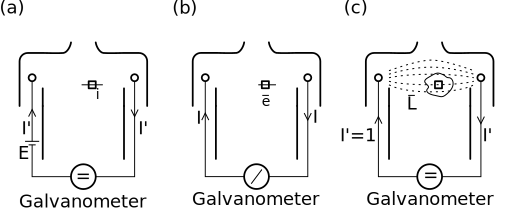
\includegraphics{figures/intro/lead_field}
\end{center}
\caption[Diagram of the Reciprocity Principle and the Lead Field]{
\label{fig:intro:ecg:lead_field}
Diagram of the Reciprocity Principle and the Lead Field.
(a) Inducing a current in the lead $l$, between the terminals of the
galvanometer causes an electric field which causes a current $i$ to flow through
the small element (square) in the heart.
(b) An electric field, $\vec{e}$, generated by the small element causes a current
I to flow in $l$ causing the galvanometer to read the potential difference $E'$.
If $E'$ equals $E$ then $I$ equals $i$.
(c) The lead field, $\vec{L}$, is defined from the current which flows in each
small unit of the heart when the current introduced is the unit current.

}
\end{figure}

To derive the lead field, we consider a unit current flowing in a
lead $l$~(figure~\ref{fig:intro:ecg:lead_field}).
The resulting flow of current through the body will have a certain magnitude and
direction at every point; it is a vector field.
This vector field is called $\vec{L}$, the lead field.
If one considers a small volume in the heart region of the torso then the
presence of the lead field, $\vec{L}$, will set up an electric field in the
volume, $\vec{e}$.
The principle of reciprocity means that if instead the electrical activity of
the heart creates an electric field, $\vec{e}$, in the heart region then a unit
current will flow through the lead $l$.
The principle of superposition allows the contributions of many such small
volumes, each containing their own field, $\vec{e_1},\cdots,\vec{e_n}$, to
create a current, and thus a potential difference in $l$.


\subsection{The Twelve Lead Electrocardiogram}

The twelve lead electrocardiograph is the initial basis of almost all cardiac
diagnosis.
It started out as the three einthoven leads.
The electrodes are located (figure~\ref{fig:intro:ecg:leads})(a)) on the left
shoulder, L, the right shoulder, R, and the feet (typically the left leg), F.
Lead I (\ref{eqn:intro:leads:i}) uses R as the negative terminal and L as the
positive terminal.
Lead II (\ref{eqn:intro:leads:ii}) is formed between R as the negative terminal
and F as the positive terminal.
Lead III (\ref{eqn:intro:leads:iii}) is formed between L as the negative terminal
and F as the positive terminal.

\begin{figure}
\begin{center}
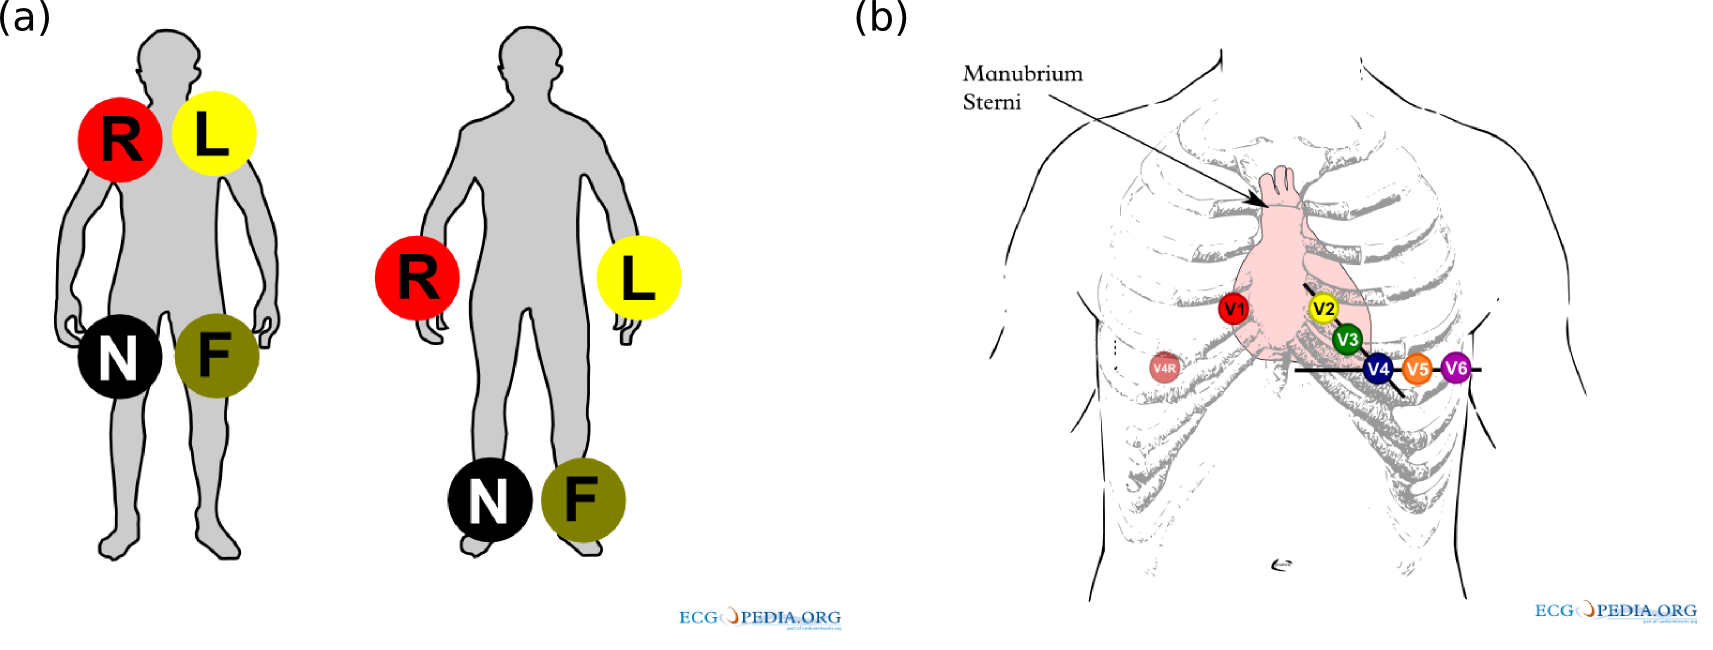
\includegraphics{figures/intro/ecg_leads}
\end{center}
\caption[Lead placements for the 12 Lead ECG]{
\label{fig:intro:ecg:leads}
Lead placements for the 12 lead ECG.
(a) Placement of the three limb leads, L, R and F, as well as the ground
electrode N.
(b) Placement of the six precordial electrodes, $\text{V}_{\text{1--6}}$.

Images are reproduced from the ECGpedia~\cite{ecgpedia}.
Both are kindly released under a Creative Commons
Attribution-Noncommercial-Share Alike 3.0 Netherlands License.
}
\end{figure}

Wilson~\cite{Wilson1934}, in the 1930s, introduced an indifferent
electrode,  constructed by averaging the potentials at the three limb
electrodes (\ref{eqn:intro:leads:wct}).
This is the Wilson's central terminal (WCT).
They introduced three new `unipolar' leads, all of which use the WCT as the
negative terminal.
For the positive terminal, VL uses the L electrode, VR the R electrode and VF
the F electrode.
Later Goldberger~\cite{Goldberger1942}\ noted that be removing the electrode used
as the positive terminal from the calculation of the central terminal for the
negative electrode, the amplitude of the lead would be 50 per cent larger than
that of the normal unipolar leads.
These leads were termed the augmented unipolar leads, denoted by the prefix of
an `a'.
The aVL (\ref{eqn:intro:leads:avl}) leads uses L for the positive terminal and
the average of R and F for the negative terminal.
The aVR (\ref{eqn:intro:leads:avr}) leads uses R for the positive terminal and
the average of L and F for the negative terminal.
The aVF (\ref{eqn:intro:leads:avf}) leads uses F for the positive terminal and
the average of R and L for the negative terminal.
The set of leads consisting of I, II, III, aVL, aVR and aVF are known as the
limb leads.
The superior limb leads are I, aVL, aVR and the inferior are II, III, aVF.

The precordial leads were introduced by Wilson~\cite{Wilson1944}\ to provide a
better view of the electrical activity of the heart from the chest.
They are all unipolar leads which use the WCT for the negative
terminal.
For the positive terminal they use one of the six precordial electrodes
(figure~\ref{fig:intro:ecg:leads})(b), the locations of which are described in
many textbooks (e.g.  \cite{Hampton2008}).
The first precordial electrode, which is the positive terminal of
$\text{V}_{\text{1}}$ (\ref{eqn:intro:leads:v1}) is located to the right of the
sternum, in the fourth intercostal--between the ribs--space.
The second precordial electrode, which is the positive terminal of
$\text{V}_{\text{2}}$ (\ref{eqn:intro:leads:v2}) is located to the left of the
sternum, in the fourth intercostal space.
The third, the positive terminal of $\text{V}_{\text{3}}$
(\ref{eqn:intro:leads:v3}) is located between the second and fourth precordial
electrodes.
The fourth ($\text{V}_{\text{4}}$, \ref{eqn:intro:leads:v4}) is located on the
left midclavicular line, in the fifth intercostal space.
The fifth ($\text{V}_{\text{5}}$, \ref{eqn:intro:leads:v5}) is located on the
left anterior axillary line, in the fifth intercostal space.
The sixth ($\text{V}_{\text{6}}$, \ref{eqn:intro:leads:v6}) is located on the
left positerior axillary line, in the fifth intercostal space.

The voltage, $V$, across each lead can be written as
\begin{subequations} \label{eqn:intro:leads}
\begin{align}
V_{I}  = &\phi_{L} - \phi_{R}\label{eqn:intro:leads:i}\\
V_{II}  = &\phi_{R} - \phi_{F}\label{eqn:intro:leads:ii} \\
V_{III}  = &\phi_{L} - \phi_{F}\label{eqn:intro:leads:iii}\\
V_{WCT}  = &\frac{\phi_{L} + \phi_{R} + \phi_{F}}{3}\label{eqn:intro:leads:wct}\\
V_{aVL} = &\phi_{L} - \left(\frac{\phi_{R} + \phi_{F}}{2}\right) \label{eqn:intro:leads:avl}\\
V_{aVR} = &\phi_{R} - \left(\frac{\phi_{L} + \phi_{F}}{2}\right)\label{eqn:intro:leads:avr} \\
V_{aVF} = & \phi_{F} - \left(\frac{\phi_{R} + \phi_{L}}{2}\right)\label{eqn:intro:leads:avf}\\
V_{1} = & \phi_1 - V_{WCT} \label{eqn:intro:leads:v1}\\
V_{2} = & \phi_2 - V_{WCT} \label{eqn:intro:leads:v2}\\
V_{3} = & \phi_3 - V_{WCT} \label{eqn:intro:leads:v3}\\
V_{4} = & \phi_4 - V_{WCT} \label{eqn:intro:leads:v4}\\
V_{5} = & \phi_5 - V_{WCT} \label{eqn:intro:leads:v5}\\
V_{6} = & \phi_6 - V_{WCT} \label{eqn:intro:leads:v6}
\end{align}
\end{subequations}
where $\phi_x$ is the potential measured at electrode $x$.

As there are only 9 electrodes in the twelve lead ECG, there are only 8
potential differences which can be uniquely determined.
These are, by convention, leads I, II and $\text{V}_{\text{1--6}}$.
The value of the other limb leads is that they provide a view of the activity of
the heart from different angles, thus what might be unclear on one lead can be
obvious on another.
This concept of lead angles creates what is known as the hexaxial reference
system (\cite{Lipman1994}, pp 94., amongst others), illustrated in
figure~\ref{fig:intro:ecg:hex}.
The angle at which each lead points is the direction of the positive terminal.
Lead I, which is nominally horizontal, is at \degr{+0}.
Under the hexaxial system, Lead II has an angle of \degr{+60}\ and lead III,
\degr{+120}.
The unipolar limb leads (both augmented and not) have angles of \degr{-30}\ for
aVL, \degr{+90}\ for aVF and \degr{-150}\ for aVR.

\begin{figure}
\begin{center}
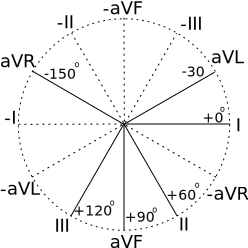
\includegraphics{figures/intro/hexaxial}
\end{center}
\caption[Hexaxial Reference System]{
\label{fig:intro:ecg:hex}
Diagram of the hexaxial reference reference system, showing the nominal
directions of the 6 limb leads.
The positive senses of the leads are in bold, the negative are dashed.
\degr{+0}\ is horizontal and to the left, in the reference frame of the body.
}
\end{figure}

\subsection{The ECG Waves}

\begin{figure}
\begin{center}
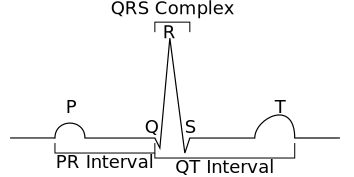
\includegraphics{figures/intro/schematic_ecg}
\end{center}
\caption[Schematic ECG]{
\label{fig:intro:ecg:schematic}
A schematic representation of the ECG in lead II.
Shown are the P-wave, the QRS complex and the T-wave.
Also indicated are two important time periods; the PR interval and the QT
interval.
}
\end{figure}

In terms of the ECG, a `wave' is a deflection from the baseline observed in the
lead.
There are five standard waves in the ECG; P, Q, R, S and T.
The origin of the names of these waves is a matter of some
controversy~\cite{Hurst1998}, but whatever their origin, they are now enshrined
in the literature.
A schematic representation of the ECG waves is shown in
figure~\ref{fig:intro:ecg:schematic}.
Each of the waves is the result of the electrical activity in a particular part
of the heart.
Positive deflections are those which are above the baseline and negative ones
below.

The P-wave is caused by the depolarisation of the atria.
It has a relatively low amplitude because the atria are small and thin walled
compared to the ventricles, so there are not that many cells which can generate
the wave.
It tends to last from \ms{100} to \ms{120}.

The QRS complex is associated with the ventricular depolarisation.
It is a collection of up to three waves.
Any negative deflection which preceeds the R wave is the Q wave.
The R wave is the first positive deflection.
The S wave is the first negative deflection after the R wave.
A QRS complex does not need to have all three of the QRS waves present.
The QRS complex tends to have the largest magnitude in the ECG and lasts
approximately \ms{100}.

The T wave is associated with the ventricular repolarization.
It occurs some time after the QRS complex.
The $\text{T}_{\text{P}}$, caused by the atrial repolarization is not normally
visible on the ECG for a number of reasons.
It is very small in magnitude, it is also often masked either by the QRS complex
or by so called `baseline correction' algorithms which use the PR interval to
determine a `zero' for the ECG.

The axis of a wave is direction in which it has maximum amplitude.
This is determined using the hexaxial reference system.
A normal QRS complex (\cite{Lipman1994,Katz2006}) has an axis between \degr{-30}\
and \degr{+110}.
A normal P wave has an axis between \degr{+0}\ and \degr{+90}.

\subsubsection{Describing an ECG Wave}

\begin{figure}
\begin{center}
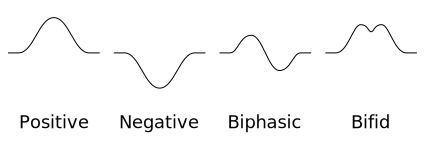
\includegraphics{figures/intro/ecg_waveforms}
\end{center}
\caption[ECG Morphology]{
\label{fig:intro:ecg:waveforms}
A schematic representation of P- and T-wave morphology.
From left to right, a positive, negative, a positive--negative biphasic and a
positive bifid wave are shown.
}
\end{figure}

The terminology used to describe ECG waves is illustrated in
figure~\ref{fig:intro:ecg:waveforms}.
Positive waves, those with a deflection above the baseline, and negative waves,
with a deflection below the baseline have already been explained.
The P- and T-waves can have more complex morphology however.
A P- or T- wave which shows both positive and negative deflections is termed
biphasic.
A positive--negative biphasic deflection is one which is first positive and then
negative.
A wave for which the converse is true is called negative--positive.
A wave which is entirely positive, or negative, but that has a notch in the
middle is described as bifid.

\subsection{The Vectorcardiogram}

Orthogonal lead systems, intended to measure the three independent components of
the heart's dipole, were first proposed in the middle of the 20th century.
Frank~\cite{Frank1956}, after experiments on physical models of the torso,
proposed his `corrected' orthogonal system.
This was corrected in the sense that the three lead vectors measured were
truly orthogonal and of equal magnitude in each of the three directions.
This included the influence of internal conductive regions and variability in
heart location.
The system uses 7 electrodes.
The three vectors chosen are X, a horizontal vector, positive to the left.
The Y vector is vertical and is positive towards the feet.
The Z vector is horizontal and positive towards the back.

\begin{figure}
\begin{center}
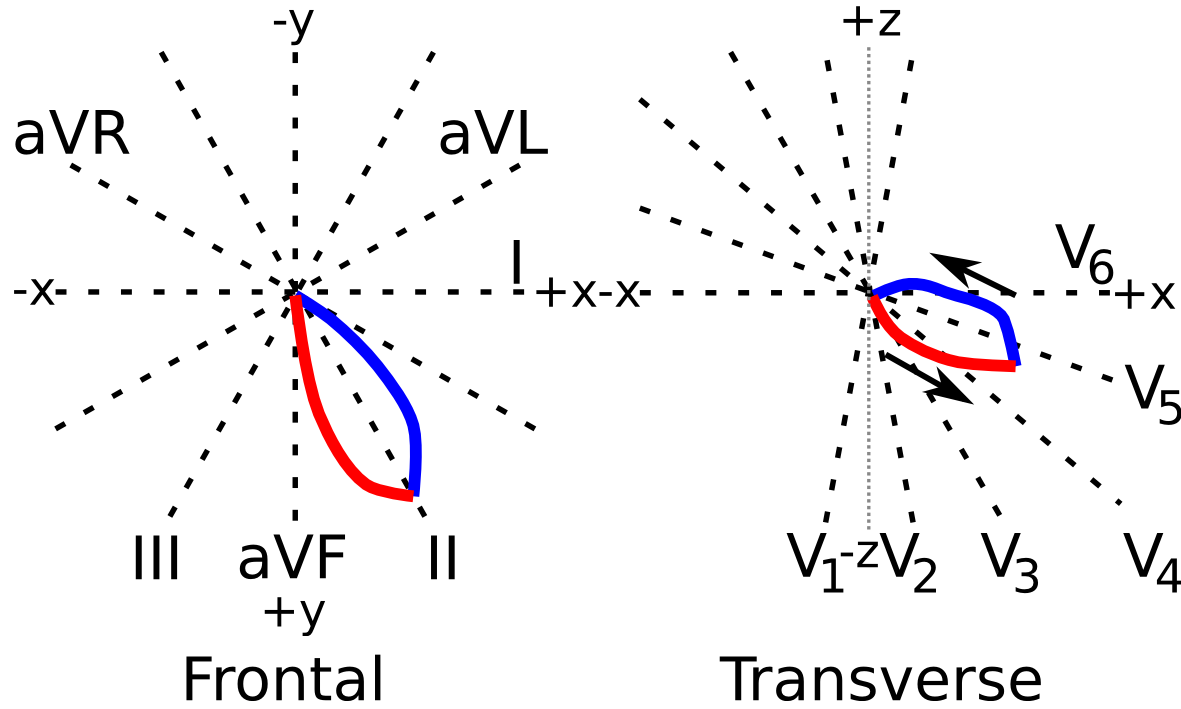
\includegraphics{figures/intro/vector_loops}
\end{center}
\caption[Schematic Vector Loops]{
\label{fig:intro:ecg:planes}
Schematic vector loops showing the relationships of the leads to the frontal and
transverse plane.
The lines of the leads are indicated in heavy-set black lines, the axes in grey
dots when they do not coincide with a lead.
The schematic loops are shown in red and blue, with arrows to indicate the
direction of inscription.
The afferent, or outgoing, limb of the loop is shown in red.
The efferent, or incoming, limb of the loop is shown in blue.
}
\end{figure}

The vectorcardiographic leads can be combined to visualize the electrical
activity of the heart in three planes.
These are the frontal plane, which combines Y and X, the transverse plane, which
combines X and Z, and the sagittal plane, which combines Y and Z.
The frontal plane is the one in which the limb leads measure, whilst the transverse plane
can be related to the precordial leads, as illustrated in
figure~\ref{fig:intro:ecg:planes}.

Dower~\cite{Dower1980}\ proposed a series of coefficients for the three Frank
leads that would convert the Frank leads into the standard 12 lead ECG.
However, the Frank leads are not recorded in common clinical practice.
To remedy this fact, Edenbrant and Pahlm~\cite{Edenbrandt1988} (and others, for
example~\cite{Uijen1988}), proposed an `inverse dower' transformation.
The inverse dower transform is a set of $8\times3$ coefficients
(table~\ref{tbl:intro:ecg:inverse_dower}) which are used to multiply the eight
independent components of the twelve lead ECG (I, II, $\text{V}_{\text{1--6}}$)
to form the three Frank leads.


\begin{table}
\caption[Inverse Dower Factors after Edenbrandt and Pahlm]{
\label{tbl:intro:ecg:inverse_dower}
Factors to construct the Frank VECG from the standard 12 lead ECG
set~\cite{Edenbrandt1988}.
Each of the 8 leads are multiplied by the given parameters to provide the
orthogonal Frank lead.
}
\begin{center}
\begin{tabular}{c c c c c c c c c}
\toprule
& $\text{V}_{\text{1}}$ &$\text{V}_{\text{2}}$ & $\text{V}_{\text{3}}$ &
$\text{V}_{\text{4}}$ & $\text{V}_{\text{5}}$ & $\text{V}_{\text{6}}$ & I & II \\
\midrule
X & $-0.172$ & $-0.073$ & $0.122$ & $0.231$ & $0.239$ & $0.193$ & $0.156$ & $-0.010$ \\
Y & $0.057$ & $-0.019$ & $-0.106$ & $-0.022$ & $0.040$ & $0.048$ & $-0.227$ & $0.886$ \\
Z & $-0.228$ & $-0.310$ & $-0.245$ & $-0.063$ & $0.054$ & $0.108$ & $0.021$ & $0.102$ \\
\bottomrule
\end{tabular}
\end{center}
\end{table}




\subsection{Body Surface Potential Mapping Arrays}

Body surface potential mapping arrays consist of many electrodes distributed
over the body and recorded simultaneously.
These allow the whole of the body surface potential to be examined and
to be used to establish diagnostic
criteria (for example, \cite{Dubuc1993,SippensGroenewegen1998}).
Mapping systems are also important for so called `inverse solutions', where the
cardiac sources are estimated from the external potentials (for example,
\cite{Ramanathan2006}).
They are also used for the construction of new lead sets (for example,
\cite{Sobieszczanska2007}).
Arrays of anywhere from 16 to over 200 electrodes have been used in such
studies.

\section{The Forward Problem}

The so-called `forward problem' seeks to find a relationship between the
electrical activity in heart and the potentials observed outside the heart,
most usefully on the surface of the body.
When looked at another way, it is a method of finding the lead field, $\vec{L}$,
for a given body.
The problem has been approached in a number of ways; experimentally, clinically
and numerically.

\subsection{Uses of the Forward Problem}

The original investigations into the forward problem very much concerned
themselves with finding $\vec{L}$.
They sought to refine the understanding of such concepts as the einthoven
triangle and the precordial electrodes and to more closely relate the differing
potentials observed with what was happening in the heart.
The experiments in the forward problem led to the lead field theory of McFee and
Johnson~\cite{McFee1953}\ and the Frank vectorcardiogram~\cite{Frank1956}.

Modern investigators of the forward problem use the solutions to perform similar
investigations, such as the development of new lead systems~\cite{Ihara2007}.
Forward solutions are also used for investigations into ischeamia, ventricular
and atrial fibrillation, conduction defects, amongst many.
Forward solutions also form the basis, or are used in the refinement, of inverse
solutions.

\subsection{A Brief History of the Forward Problem}

As has been mentioned, the initial uses of the forward problem were to determine
how the activity of the heart related to the leads.
These initial models tended to be real and physical models.
Towards this end, one of the first models constructed was by Burger and van
Milaan~\cite{Burger1946}, who constructed a one third life-size model of the
torso, filled with electrolyte solution.
The model had a cork spine and sandbags to represent the lungs.
The measurements from this model formed the basis for their refinements to the
lead theory.

Of the early mathematical models Brody~\cite{Brody1956}\ is one of the most
significant.
His was a model of the influence of the highly conductive blood masses of the
heart on the measured electrical field.
The `Brody Effect' is still used in literature today.

In the 1960s, numerical models of the torso started to
appear~\cite{Barr1966,Barnard1967}.
These initial models generally had a handful of dipoles, or even just one, to
represent the heart.
These were used to investigate the influence of dipole position and
heterogeneities on the body surface potential.

In 1971 Rush~\cite{Rush1971} published his torso model.
This was probably the ultimate torso model, literally and figuratively.
The model was twice lifesize and incorporated internal inhomogeneities
representing lungs, heart, heart blood, great blood vessels, liver, fat,
skeleton and anisotropic skeletal muscle--though the model could be used without
them as well.
The cardiac activity was represented by a number of dipole sources which were
located in the heart region of the torso.

In the 1980s, models of the heart and the torso gained more
sophistication~\cite{Gulrajani1983,Horacek1987}, though they were still generally
ventricular models, not models of the whole heart.
Models of this era routinely used 10s of dipole sources.
These models still did not include even primitive electrophysiology models,
although towards the end of the decade, propagation of the excitation wavefront
was being modeled~\cite{Aoki1987}.

Moving to the nineties and the turn of the millenium, the availability of
medical imaging tools such as CT and MRI scans allowed more accurate models to
be constructed~\cite{Weixue1993,Weixue1996}.
This is also when the first models began to appear which incorporated the
atrium~\cite{Weixue1996,vanDam2005}.
Many of the models published in this era use myocyte models to simulate the
propagation, some even using biophysically detailed models.

\subsection{Numerical Approaches}
\label{sec:intro:forward:numerical}

Numerical solutions to the forward problem involve solving Maxwell's equations
within the torso.
The same assumptions which were made for the lead field theory
($\S$\ref{sec:intro:ecg:lead_theory}) are valid here.
To reiterate them briefly, they state that the body is a linear volume
conductor.
There are no inductive or capacitive effects.
Furthermore, due to the finite (and small) size of the body, there are no
propagation effects to consider.
The field in the body, $\vec{E}$ is therefore given by
\begin{equation}
\label{eqn:intro:forward:maxwell}
\vec{E} = -\nabla\phi
\end{equation}
where $\phi$ is a scalar potential field.
Current flow in the torso under these conditions is given by Ohms law, which
states the total current flow, $\vec{J}$, is
\begin{equation}
\label{eqn:intro:forward:ohm}
\vec{J} = \mathbf{\sigma}\vec{E} + \vec{J^i}
\end{equation}
where $\mathbf{\sigma}$ is the conductivity tensor and $\vec{J^i}$ is an
impressed, or applied, current density which is generated by active sources,
i.e. the heart.

Since the total current flow is solenoidal, i.e. the net current flow into and
out of a volume is zero, via (\ref{eqn:intro:forward:ohm}) we have that
\begin{equation}
\label{eqn:intro:forward:ohm2}
\nabla\cdot\vec{J} = 0 = \nabla\cdot\left(\mathbf{\sigma}\vec{E} + \vec{J^i} \right)
\end{equation}
This can alternatively be written as
\begin{equation}
\label{eqn:intro:forward:poisson}
\nabla\cdot\vec{J^i} = \mathbf{\sigma}\nabla^2\phi
\end{equation}
If the body is homogeneous and isotropic, it becomes
\begin{equation}
\label{eqn:intro:forward:poisson2}
\nabla^2\phi = \frac{\nabla\cdot\vec{J^i}}{\sigma}
\end{equation}
which is Poisson's equation.

Finding $\phi$ for a given $\vec{J^i}$ can be achieved using a volume or
boundary based approach.
Volume based approaches \cite{Seger2004,Klepfer1997,Keller2007}\ involve dividing the body
up into volumes of different conductivity.
There is also the recent `Meshless Finite Element Method'~\cite{Li2007a}, which
uses the nodes of a typical finite element method, but not the elements.
The solution for $\phi$ is found using a finite element or finite difference
method.
Boundary element based approaches
\cite{Barr1966,Clayton2002,Gulrajani1989,Weixue1996}\ divide the torso into
regions of isotropic and uniform conductivity.
The potential, $\phi$, is found on the surfaces of these regions.

Volume based methods allow for a more complex model.
Interior volumes can have internally varying or even anisotropic conductivity.
They tend to be much more computationally intensive to solve, however, because
the problem space is still three dimensional.
In addition, the required element size can be quite small, especially for finite
difference approximations.
Keller~\cite{Keller2007}\ used a model with more than ten million torso
elements, for example, whilst the finite element model used by
Klepfer~\cite{Klepfer1997}\ has approximately one million elements and 168,000
nodes.

Boundary element based methods by contrast tend to be much simpler to solve.
Typical model sizes are of the order of a thousand to ten thousand elements, as
they reduce the problem space to a series of two dimensional surfaces.
This reduces the computational effort required.
However, since the solution is only computed at the surfaces, regions can only
be uniform and isotropic.






\section{A Cardiac Simulation Toolkit}

Cardiac simulation toolkits have existed in one form or another for some
time and include both commercial and open source 
Several cardiac simulation systems have previously been released, one of
the first of which is the OXSOFT HEART~\cite{Noble-1999}.


   \chapter{Constructing a Cardiac Simulation Toolkit}

\section{Simulation Environment}

The simulation environment provided by the cardiac toolkit is intended to be as
portable as possible, so that numerical experiments may be run on whichever
platforms are appropriate.  To this end, all the data input structures are based
on open standards, or simple binary formats.  The output formats provided by the
various driver programs are also in simple binary or ASCII formats, to allow
them to be easily visualized with both commercial and open source visualisation
tools.  The results presented later in this chapter were performed on desktop
computers with a XX GHz Althon X2 chip and 1 GB RAM and on Horace, the local HPC
facility.  Horace has 24 compute nodes, each one consisting of four Intel Itanium2
Montecito Dual Core 1.6GHz processors, 16GB RAM and up to 512GB of local scratch
space.  The nodes are connected by a high speed Quadrics QsNetII
interconnect~\cite{horace}.  Horace provides compilers for both Fortran and C,
and for both the MPI and OpenMP parallelization libraries.

\subsection{Implementation}

The experimental protocol drivers and the cellular models were implemented in
the C programming language, although much of the supporting code and
supplementary tools were implemented in the ruby programming language.  The
cellular models currently implemented are based on the Hodgkin-Huxley formalism,
although there is no fundamental reason why a Markov chain based model could not
be included.  Inter-cellular coupling for propagation of excitation over a
strand or tissue was implemented using the monodomain equations.

\subsubsection{Cellular Models}

The cellular model used for much of the developmental process was the
Courtemanche et al. human atrial myocyte model~\cite{crn98}.  Also currently
implemented are the Nygern et al. human atrial myocyte model~\cite{nygern98} and
the four variable formulation of the Fenton-Karma minimal variable
model~\cite{overo2008}.  These cellular models describe the behaviour of a cell
using coupled systems of non-linear ordinary differential equations.  The ODEs
represent the concentrations of intra- and extra-cellular ion species and the
flow of current through ionic channels in the cell membrane or between
intra-cellular compartments, or their notional equivalents in the case of minimal
variable models.

These equations were generally solved using the simplest time-stepping method
available, the explicit Euler method.  To improve performance and stability,
some variables were integrated using the Rush-Larsen method.  More complex
integration schemes were tried, but did not significantly improve performance to
compensate for the greater complexity.

\subsubsection{Monodomain Equations}

The monodomain equations were used to couple multiple cells together to describe
a tissue over which excitation could be conducted.


A discussion of the merits of the monodomain and bidomain equations can be found
in the introduction.


\subsubsection{Strand Model}

The 1D strand model is used for several experimental protocols, as
a computationally cheaper alternative to a full tissue model.  The 1D strand
model consists of a number of nodes, typically 200 or 300, which are coupled
electrically at the ends of the cells.  The electrical activity at each node is
modelled via a cellular electrophysiology model and electrical conduction between the
nodes is handled via a 1D formulation of the monodomain equations, with no
flux boundary conditions.

\subsubsection{Sheet Model}

The 2D sheet model is used for several experimental protocols, as well as more
general numerical experimentation.  The 2D sheet model consists of a grid of
nodes, coupled electrically along the cardinal directions of the grid.  The
electrical activity at each node is modelled via a cellular electrophysiology
model.  Conduction of the electrical excitation between the nodes uses the
mono-domain equations with no flux boundary conditions applied at all tissue
boundaries.  The square sheet model, used in several of the numerical
experimental protocols described later, is typically 375x375 nodes, representing
140625 cellular models.  Two dimensional idealizations of physiological
preparations can have many more nodes, to on the order of $10^{6}$ cellular
models.  These idealizations can often be quite irregular and so to allow easy
and effective partition of workload across multiple processors, the tissue map
is decomposed into a 1D array which contains references to the neighbouring
cells.


\subsection{Parallelization}

Some parts of the toolkit require the modelling of large numbers of cells, on
the order of tens or even hundreds of thousands of cellular models in two
dimensional sheets.  Solving all the equations involved takes a significant
amount of time and so it is desirable for such simulations to be parallelized so
that the work involved can be split over several processors.  This can have
advantages beyond merely having eight rather than one cores worth of
computational cycles working on solving the equations.  Splitting the work over
multiple cores can also increase the amount of cache available, allowing for
more efficient operation of the solvers.

For the toolkit, the OpenMP~\cite{OpenMP} parallelization library was chosen.
This implements the shared memory parallelism paradigm.  Using the shared memory
paradigm is simpler, due to the lack of explicit communication calls, and can be
faster, as there is merely memory access involved, rather than communication
over an network or other interconnect.  Finally, a program written using OpenMP
can, with some care, also be compiled serially if an OpenMP compiler is not
available.  Whilst a program implemented using a non-shared memory paradigm,
such as using the MPI library, would allow it to be executed on potentially more
processors which would potentially offer faster run times, in practice the eight
core shared memory system Horace provides as a compute node was general found to
be sufficient for the task.

\subsection{Optimisation}

The toolkit uses several techniques to optimize the computations performed,
reducing the number of processing cycles required to compute the results needed
for publication.  These optimisations are generally built around the principle
of ``No code is faster than no code'', although it might be more accurate to say
``No code execution is faster than no code executed''.  To explain this idea
another way, it is that no combination of compiler flags can compete with a
sensible choice of algorithm which minimizes the number of computational steps
to be performed or the amount of data to be written to a file.  This is not to
say that the compiler is are unimportant, but that it is merely the start of
optimisations, rather than the final step.

\subsubsection{The Compiler}

The toolkit has been compiled using the GNU C compiler (gcc)~\cite{gcc}, the
Intel C compiler (icc)~\cite{icc} and the Sun microsystems .  All three have
OpenMP implementations available and all three are capable of performing a
number of optimisations, controlled via flags.  The most important aspect of the
optimisations is that they should not alter the behaviour of the floating point
handling, as this could have significant impact on the final result computed.
Despite this caveat, the results of applying certain optimisation flags can be
quite significant.

\subsubsection{Caching of Computed Values}

Moving beyond the compiler, one of the simplest forms of optimisation is to only
calculate each value once, if at all possible.  This can be done in a number of
ways and the toolkit developed here implements two such methods for saving
computational time.

State saving is one of the most direct ways of caching computed values.  At a
particular point in the simulation, all of the state variables of the
system are copied into an intermediate location.  This might be a file on disk or
to another location in memory.  If the state is written out to a file, that file can
be used as a `save point', allowing the simulation to be continued from that
point in the future, ensuring work is not wasted.

When copied to another memory location, this allows the program to return to
that point in the future.  This is useful in modelling many experimental
protocols, which often call for a number of `conditioning' pulses to allow the
cell or model to settle.  The state can be saved after the conditioning pulses
and then the actual tests can be performed quickly, saving the execution of
several seconds of simulated activity.  This technique should obviously only be
used for cells in the Hodgkin-Huxley formalism which are deterministic and thus
give identical results whether the state is saved or not.  Using such a
technique with a cell that has a number of stochastic components could
potentially affect the quality of the results.

The second way in which caching can be employed is in the creation of `lookup
tables'.  A lookup table is a pre-computed table of the values an expression can
take.  When the expression would normally be evaluated, the table is used
instead, replacing what might be a complicated expression with a single array
lookup.  For lookup tables to be efficient to pre-compute, the tabulated
expression should depend on only one variable and should be sufficiently
`complex' expression, such as one involving the computation of mathematical logs
or exponentials.  The expression should depend on only one variable as the
pre-computed table has to be indexed over each variable the computation depends
on and even dependence on just two variables would increase the number of table
entries required by thousands or millions.  The requirement for complexity is a
little more obvious, as any optimisation can only save as much time as the
original series of operations took.  With these limitations in mind, it is still
possible to find many candidates for pre-computation in typical cardiac cell
models, most notably the activation and inactivations of voltage dependent
gates.  This technique is typically only worthwhile performing in the case of
tissue simulations where the benefits can be shared amongst all the cells since
pre-computation can be quite expensive, destroying any efficiency gains made
through their use for single cell simulations.

\subsubsection{Binary Searches}

Several of the experimental protocols provided by the toolkit are intended to
determine the value of a parameter which causes a particular condition to be
fulfilled, such as a successful excitation of the cellular model after
progressively shortening stimulus intervals.  This value we will call the
critical value. In real experiments, ones involving actual cardiac tissue, the
typical experimental protocol would involve stimulating the tissue at
sequentially shorter intervals, until no stimulation was provoked.  This might
involve stimulating the cell thousands of times, which would be expensive
computationally to model exactly.  Instead, a binary search for the critical
value can be performed, using the pseudo-code shown here.


To explain in words, first two guesses are made; the high guess, which is the
maximum value that the critical value can take, and the low guess, the minimum
it is presumed to take.  The simulation is then run with the parameter set at
the average of the low and high guesses--the current guess.  If the test is
successful, the critical value evidently lies somewhere between the low guess
and the average, and so the high guess is set to the current guess.  Conversely,
if the test is unsuccessful, the critical value is obviously above the current
guess, and so the low guess is set to the current guess.  The simulation is then
repeated with the average of the new high and low guess.  Using this algorithm,
the search space is halved with each iteration, swiftly finding the critical
value.  For example, to find a parameter somewhere in the range of 0--1000~ms to
the nearest millisecond requires just 10 iterations of the binary search
algorithm, but might take hundreds of iterations with sequential searching.

One important thing that must be considered when using binary searches is that
there is only one critical value in the range considered or else the algorithm
will give unpredictable results.  In practice, this limitation is often quite
easy to work within.

\subsubsection{Adaptive Step}

Adaptive step mechanisms are employed in the toolkit when there is a need to
provide output over a wide range of times, when the slope of the graph is not
constant over the range to be graphed.  This is very common in the modelling of
cardiac cells, which often show an exponential dependence of various parameters
on the  stimulus interval, and are graphed over a range of hundreds or thousands
of milliseconds.  A step that sufficient to track the curve at the upper limits
of the range will completely fail at the steeper slow of the lower limits,
whilst a step that will track the curve for the lower limits will result in
unnecessary work being done at the upper end of the range.  To alleviate this
problem, an adaptive stepping mechanism is used, as shown in this pseudo-code.

First, the measurement is performed at the largest desired point.  The interval
is then reduced by the step, and the measurement is performed again.  The
difference in the measurements is calculated and compared to the desired maximum
delta.  If the difference is acceptable, the interval is once more reduced by
the step, and the measurement taken once more.  If the difference is too great,
then instead the step size is halved and the measurement repeated.  If the
difference is now acceptable, then the interval is reduced by the new step and
the experiment proceeds.  If it is not, then the step size is once more halved.
The step size used is therefore always appropriate to the slope of the curve and
a smooth graph results.  Additional logic, not shown in the pseudo-code, is used
to ensure the step size does not become too small, and to terminate the graph at
the lower end of the range.

Since curves can increase or decrease the absolute difference between the two
values is compared.

\subsubsection{Parallel Input/Output}

Input and output for simulations is obviously essential if they are to be of any
use.  This input and output can involve the reading or writing of many megabytes
or gigabytes of information over the course of a simulation, often in a variety
of different formats.  This most significant for sheet simulations and it is
those that we consider here.

Data input is typically not that significant a cost for
simulations, as whilst various simulation maps and saved states be quite large,
the cost is typically only paid once.  Data output is often required at numerous
points throughout the course of the simulation since almost all simulations are
performed to examine the time evolution of the cardiac system.  Many simulations
will output the value of state parameters, most commonly the voltage, at all
points in the tissue every few milliseconds of simulated time.  Other state
variables might also be desired and the toolkit also offers `live visualization'
of two dimensional sheets via output of images in the GIF format.  In addition,
the whole state is output regularly, to allow simulations to be resumed at a
later point in time.  This output usually stops all simulation whilst it is
being written to disk, time during which the processors are typically idle.  By
allowing multiple threads to output in parallel, the cost of outputting multiple
files can be reduced to the cost of outputting one.


\section{Experimental Protocols}

The toolkit developed provides a number of experimental protocols to use with
the cellular models to quantify the electrophysiological behaviour of the
modelled cells.  The provided protocols include the action potential duration at
90\% repolarisation (APD90) and the action potential (AP) profile; the
APD90 and APD50 restitution; the effective refractory period (ERP) restituion
(ERPr); the conduction velocity (CV) restitution (CVr); the temporal
vulnerability window to unidirectional conduction block (VW) and a flexible
system for specifying two dimensional sheet experiments, including the
initiation of re-entry via wavebreak protocols and computation of the spatial
vulnerability window.

\subsection{Action Potential Duration}

\subsection{Action Potential Duration Restitution}

The toolkit calculates the APDr via a standard S1--S2 protocol used in both
numerical simulations and also in physiological experiments.  The APDr is used
as a measure of how the cell responds to stimulations at different rates.  The
protocol used is shown here.


The cellular model is paced nine times with a stimulus close to the threshold
value at a given frequency or BCL.  At this point, the state is saved for the
paced cells.  The tenth S1 stimulus is then given, followed by the S2 after a
varying DI, which is reduced via an adaptive step to record the relationship
between DI and the APD of the following AP.  The toolkit also determines useful
parameters such as the maximal slope of the restitution curve, which can be
related to the stability of spiral waves within the tissue.  Both the APD90 and
the APD50 restitution can be calculated.

\subsection{Effective Refractory Period Restitution}

The ERPr is calculated by the toolkit using standard experimental protocols.
The ERP is defined as the shortest possible stimulus interval, $S2$, which still
allows a successful AP to be elicited after pacing $N$ times at a pacing
interval $S1$.  A successful AP is defined as an AP which has an amplitude
of at least 80\% of the magnitude of the preceeding AP.  To determine the rate
dependence of the ERP, it is evaluated at a decreasing $S1$ interval.

To find the ERP for a given $S1$ interval the cellular model is paced $N$ times
at that interval. The state is saved just before the $N-1$th AP is initiated.
The ERP is found via binary search.  The low guess for $S2$ is typically chosen
as zero, whilst the high guess is the $S1$ interval being tested.  The $S2$\
interval for each attempt is the average of the high and low guesses.  After the
state has been saved, the $N$th AP is initiated and its amplitude recorded.
Then \ms{S2} after, the test AP is invoked.  If it is successful, that is if it
has an amplitude of at least 80\% of the magnitude of the $N$th $S1$\ AP, then
various parameters relating to the APs are stored such as the $S1$\ and $S2$\
amplitudes and the ratio between them.  The stored state is then restored to the
cellular model and the next binary iteration is attempted, until the ERP has
been found at the desired precision.

The reduction in $S1$\ interval is stepped via an adaptive mechanism which is
used to keep the reduction in ERP between successive $S1$ intervals to below
\ms{1}.  The $S1$\ interval is reduced until it is sufficiently short that the
$S2$ interval would fall within the $N$th AP.

\subsection{Vulnerable Window}

The VW is principally a tool of numeric experimentation, based around a 1D ring
model of cardiac arrhythmia.  The VW is defined as the time period after a
stimulation during which a second stimulus elicits unidirectional propagation
along the strand.  In the case of a ring this causes retrograde propagation
which cycles endlessly.  If the stimulus is given too early, then the tissue
will still be refractory and no propagation of excitation will ensue.  If it is
given too late, then propagation will occur in both directions, which in the
ring case, results in the two excitation wavefronts annihilating each other.
Normal pacing could then resume.

The VW is found in a 1D strand model, set up as described previously.  The
strand is 200 units long and with a space step of \mm{0.1}.  The first stimulus is
given to a 3 unit (\mm{0.3}) section at one end of the strand.  The test stimulus
is given to a 4 unit (\mm{0.4}) section, usually centred in the middle of the
strand. The VW is bounded on the lower side at the time when a stimulus any
earlier would result in no propagation from a test stimulus, and on the upper
side at the time when a stimulus any later would result in bidirectional
propagation from a test stimulus.  These three cases (no, unidirectional,
bidirectional) propagation are illustrated in figure TODO.

By counting the number of APs which cross the two ends of the strand--2, 3 and
4, respectively, for the three cases in figure TODO--the result of the test
stimulus can be determined.  The two boundaries of the VW are found via binary
search, with a lower guess of \ms{0} and an upper guess of \ms{1000}.  First, the
upper bound of the VW is determined by searching for the delay when 3 APs
crossing the ends becomes 4.  The lower bound is then found by looking for the
delay at which 3 APs crossing the ends of the strand become 2.  A minor
optimisation is performed when looking for the upper bound, in that the lower
bound's high and low guesses are updated at the same time, reducing the total
space which must be searched in the second half of the program.  Before the test
stimulus is administered, the strand may be pre-paced a number of times.  In
this case the strand state is saved as the middle of the strand is depolarized
and then restored for each binary division.

\subsection{Threshold of Excitation}

The threshold of excitation is a theoretical measure, proposed by Zhang et
al.~\cite{Zhang2003}\ and used in modelling studies~\cite{Kharche2008}.  It is
defined as the minimum stimulus current which, when delivered to a cell, will
cause the cell to depolarize to a membrane potential of at least \mv{-20}.  The
threshold of excitation is calculated for a range of stimulus intervals,
successively reducing the interval until it is impossible to elicit a
depolarization of sufficient magnitude.  At each stimulus interval it is
recorded if the test pulse elicits bidirectional, unidirectional or no
propagation.

The threshold of excitation is found in a 1D strand model.  The strand is 300
units long, with a space step of \mm{0.1}.  The strand is first given $N$ S1
stimuli at a rate which allows the strand to recover between each excitation
wave.  Each S1 stimulus is delivered to the first 4 nodes (\mm{0.4}) and is
chosen to be above the threshold of excitation.  The threshold of excitation is
calculated at the 100th node and so as this node depolarises, the state for the
whole strand is cached.

The threshold of excitation is then found via binary search, with a lower bound
of \unit{0}{nS} and an upper bound chosen to be 5x the normal threshold.  The
test stimulus is delivered $\Delta t$\ seconds after the 100th node depolarises
to a group of 4 nodes centred on the 100th node.  After the test stimulus is
delivered the 4 nodes are tested for the excitation condition, attaining a
membrane potential of \mv{-20}.  If it is successful, the current stimulus
strength will assigned to the high guess.  If not, to the low guess.  In
addition, the simulation is continued to evaluate whether bidirectional,
unidirectional or no conduction of the excitation wave is evoked by the
stimulus.  The strand is then reset to the cached state and the new stimulus
strength is tested until a sufficient accuracy has been attained.  Once the
threshold of excitation has been determined for a given $\Delta t$\ the state of
the strand is once more reset to the cached state and a shorter $\Delta t$\
tested.

\subsection{Conduction Velocity Restitution}

Measurement of CV (or solitary wave velocity) itself is performed both
experimentally and numerically, as is the minimum conduction interval, which is
the shortest interval between an S1 and an S2 stimulus which still travels the
length of the strand.  This is similar to the ERP, but can also be influenced by
factors which affect the inter-cellular coupling as well as heterogeneity in the
strand.  The CV\emph{r} provides both the solitary wave velocity, the CV for a large S2
interval and the minimum stimulus interval, when the S2 interval gets too short
for an excitation wavefront to be fully propagated.

The CV\emph{r} is found in a 1D strand model, set up as described previously.
The strand is 300 units long with a space step of \mm{0.1}.  Stimuli are
delivered to a 4 unit (\mm{0.4}) length at one end of the strand at a strength
above threshold.  The strand is first given $N$\ S1 stimuli at rate which allows
the strand to recover between their application.  The S2 stimulus is then
delivered $\Delta t$\ seconds later. The conduction velocity is estimated from
the time taken to propagate between two points 100 nodes from each of the ends
of the strand, to minimize the influence of boundary effects.  The S2 time is
then stepped via an adaptive step, until a second excitation wave does not
propagate the length of the strand.


\subsection{Spiral Wave Life Span}

Spiral Wave LS is examined experimentally and numerically.  The LS of the spiral
wave and the meander pattern of the tip are both used to gain insight into the
behaviour of the tissue under conditions of cardiac arrhythmia.

Spiral waves are initiated in a square sheet of tissue $375\,\text{x}\,375$
nodes in dimension with a space step of \mm{0.1}, as described previously.  The
tissue is first stimulated along one edge via a stimulus current applied to a
row of nodes extending the length of the tissue and 3 nodes (\mm{0.3}) in width.
The planar wave is then allowed to propagate over the tissue.  Some time after
the first wave is initiated, a second stimulus is applied.  The second stimulus
is applied to half the tissue, bisecting the first wave's propagation front.
The second stimulus is a voltage clamp, with all the included tissue clamped to
a `high' potential, typically \mv{+20}--\mv{+50} for a millisecond.  The
generated spiral is then allowed to evolve until it self-terminates, the spiral
wave tip exits the tissue or until a sufficient amount of time has passed such
that the spiral can be classified as `persistent'.  The time allowed for a wave
to be classified as persistent is typically 5 or \unit{10}{s}.

The spiral wave tip traces are calculated via a standard contour based
algorithm, comparing the \mv{-60} contour line on snapshots of the electrical
activity \ms{2.5} apart.

\subsection{Spatial Vulnerability Window}

The SVW is examined both experimentally and numerically.  It is used together
with the (Temporal) VW for quantifying a mutation or condition's potential for
arrhymogenesis.  It is defined as the smallest area of tissue in a 2D sheet,
which when given a threshold stimulus in the wake of a conditioning pulse causes
at least one `figure of eight' re-entry.  A figure of eight re-entry occurs when
the excitation waves from the tips of the test area propagate back through the
centre of the area, resulting in a pair of contra-rotating spiral waves at each
end of the region.

The sheet model used for the determination of the SVW can vary in size, as the
SVW can vary substantially, depending on the electrophysiology being simulated
by the cellular models at the nodes, but the smallest used is typically
$375\,\text{x}\,375$ nodes, with a spatial resolution of \mm{0.1}.  The sheet is first given one
conditioning excitation, initiated by injecting a strip of nodes 3 nodes
(\mm{0.3}) in width with current along one edge of the sheet.  The wave is then
allowed to propagate through the tissue.  When the VW of the tissue is
positioned at the centre of the tissue, the test stimulus is delivered.  The
test stimulus is an area of tissue 20 nodes (\mm{2}) wide and of variable length.
After the test stimulus is delivered, the sheet is observed until figure of
eight re-entry is observed, or it is obvious that it will not occur.  The
protocol is then repeated with a test stimulus area of greater length.


\section{Results From Simulation Studies}

The cardiac simulation toolkit has been used in several simulation studies.
Here I present two such studies, representing different aspects of the toolkit.
The first is based on an experimental study which determined the existence of a
novel ion channel in the human atrium which caries an anion current through the
cellular membrane.  The second is principally a 2D study, concerning the effects
of Atrial Fibrillation induced Electrical Remodelling (AFER) and
electrophysiological heterogeneity in a 2D idealization of the right atrium and
the sino-atrial node.

\subsection{Anion Currents In The Human Atrium}

\subsubsection{Introduction}

In a recent experimental study, Li et al.~\cite{li2007} determined the existence
of a novel outwardly rectifying anion current in human atrial myocytes isolated
from right atrial appendages taken from patients undergoing coronary bypass
surgery.  They determined that it was separate other known ionic currents and
performed preliminary modelling based on the CRN Human Atrial Myocyte
model~\cite{crn98}.  They determined the current could be modelled by
equation~\ref{anion:eqn} with the constants given in table~\ref{anion:table}.

The total current carried by the channel, \ii{ANION}, was given by

\begin{equation}
\label{anion:eqn}
I_{ANION} = g_{ANION} \frac{V-E_{ANION}}{1-\left(c\times e^{\left(V-E_{ANION}\right)}\right)}
\end{equation}

where $g_{ANION}$ is the conductivity of the anion channel, $E_{ANION}$ is
the reversal potential of the channel and $c$ and $d$ are constants to
describe the behaviour.  All other symbols have their usual meanings.

\begin{table}
    \caption[Parameter sets for the anion sensitive current]{
        Parameter sets for the anion sensitive current \ii{ANION}\ when carrying
        \nothree\ and $\text{Cl}^{\text{-}}$\ ions.
    }
    \begin{tabular}{ l  c c}
    \label{anion:table}
    & \nothree & $\text{Cl}^{\text{-}}$ \\
    \hline
    $g_{ANION}$ & 0.37   & 0.19 \\
    $E_{ANION}$ & -45.64 & -45.64 \\
    $c$         & 0.87   & 0.94 \\
    $d$         & $8.4\,\text{x}\,10^{\text{-4}}$ &  $2.5\,\text{x}\,10^{\text{-4}}$
    \end{tabular}
\end{table}


The simulation study used the parameter set for the anion current carrying
\nothree ions.  The effects of the addition of this current to atrial
myocyte cells was quantified .  In the following
paragraphs, `control' is used to denote the unmodified CRN model and `anion' to
denote the CRN model with the additional current described by (\ref{anion:eqn})
with the \nothree\ parameter set from Table \ref{anion:table}.

\subsubsection{Methods}

The effect on the behaviour of the cells caused by the introduction of the anion
current was quantified using the simulation library described previously in this
chapter for control (no \nothree-sensitive \ii{ANION} current) and anion
(\nothree-sensitive \ii{ANION} current present) cases.  As this simulation study
was based on the CRN cell, the standard stimulus was \ms{2} in duration and
\unit{2}{nS} in magnitude.  Unless an alternative protocol is mentioned, all
simulations directly followed those set out at the start of this chapter.  None
of the simulations presented in this section involve the use of lookup tables of
voltage dependent properties.

Simulating a single cell, the following measures were quantified: the AP
profile, the restitution of APD at 50\% repolarization, \apdr[50], the
restitution of APD at 90\% of repolarization, \apdr\ and the Effective
Refractory Period restitution, ERP\emph{r}.  The maximal fast sodium activation
was quantified at the same time as the \apdr\ was computed and is the product of
the three gates in \ii{Na}, as $m^{3}hj$. In all the single cell cases, the
cell was paced 10 times before the measurement was taken, to allow simulation
parameters to settle and to adapt to any changes in pacing rate.  Storage of the
cellular state was used in all appropriate points in the simulation, to minimise
computational time.

Using a 1D strand model the temporal Vulnerability Window to unidirectional
conduction block, VW, the Conduction Velocity restitution, CV\emph{r}\ and the
threshold of excitation were computed.  The strand model used was 300 nodes long
and had a space step of \mm{0.1}.  The diffusion coefficient, $D$, was set to
$0.03125\,\text{mm}^{\text{2}}\,\text{ms}^{\text{-1}}$~\cite{Biktasheva2005}.
In all 1D simulations the strand was paced 10 times before measurement was
taken.  In all simulations this state was then cached and restored as
appropriate, as described in the algorithms section of this chapter.

Using a 2D tissue model the lifetime of re-entrant spiral waves was estimated,
following the wave-break protocol outlined earlier.  The sheet had dimensions of
$375\times375$ nodes and a space step of \mm{0.1}.  The clamp potential used
to break the wave was \mv{+50} and it was applied for \ms{1}.

\subsubsection{Results}

The AP generated by the control and anion simulations are shown in
figure~\ref{anion:ap}.  The \apd\ is relatively unchanged, but is slightly
reduced from \ms{299.6} to \ms{298.0}, whereas the \apd[50]\ is significantly
reduced, from \ms{180.1} to \ms{160.1}.  The AP profile shows a depressed plateau region (phase
2), reduced from \mv{-9.56}\ to \mv{-14.1}\ and a slightly elevated resting potential,
\mv{-79.0}\ in the anion case cf. \mv{-80.9}\ in control.  This duplicates the Li et
al.~\cite{li2007} study, and is included here only for completeness.

\begin{figure}
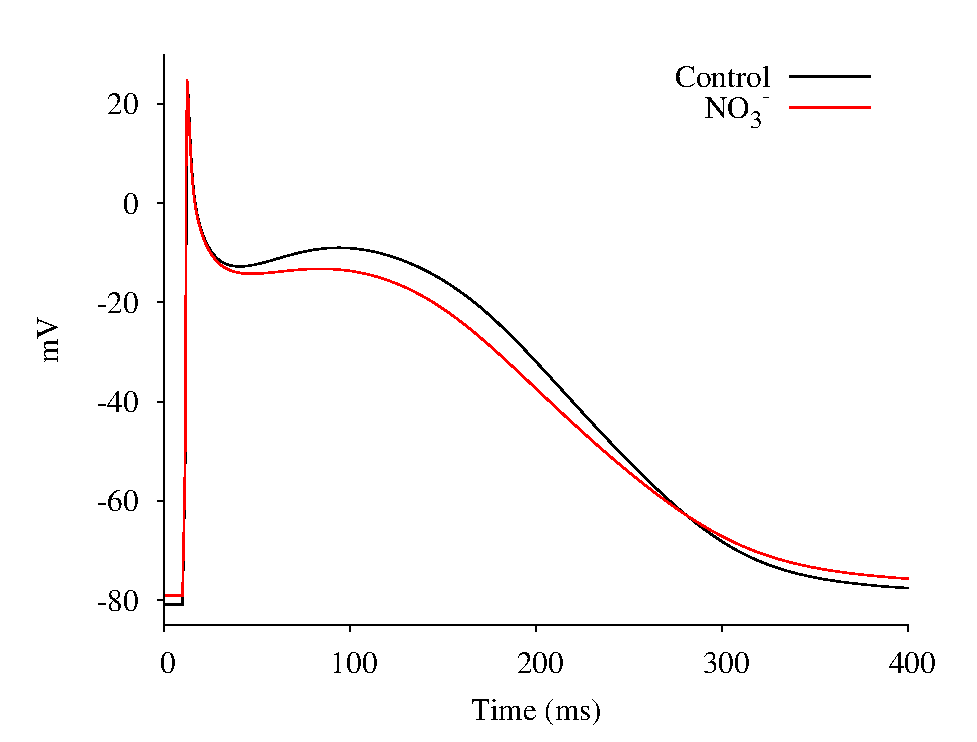
\includegraphics{figures/toolkit/anion/01_AP}
\caption[Anion Sensitive AP Profile]{\label{anion:ap} AP profile for the CRN
model in control (black) and anion (red) cases.  The inclusion of the
\nothree\ carrying current results in a small change of AP morphology, with
a depressed plateau potential and an elevated resting potential.}
\end{figure}

The APD\emph{r}\ curves produced by the control and anion cases are shown in
figure~\ref{anion:apdr50} and \ref{anion:apdr90}, for the restitution of APD at
50\% (\apdr[50]) and 90\% (\apdr) of repolarization, respectively.  The
\apdr[50]\ shows the most significant differences, with the anion
curve depressed by \ms{20} even at the largest DI, increasing to a maximum
difference of over \ms{40} at at DI of \ms{380}.  The two curves then rejoin each
other before they cross over at a DI of \ms{200}.  The \apdr\ curves, by
contrast, are very similar for control and anion cases at large (over \ms{600}) DI.
Between \msrange{100}{400}\ DI, the anion case is depressed compared to the control
case, with a difference of up to \ms{25}\ observed in the measured APDs.  At
\ms{100}, the curves rejoin one another and show a rapidly increasing slope as the
DI approaches \ms{0}.

\begin{figure}
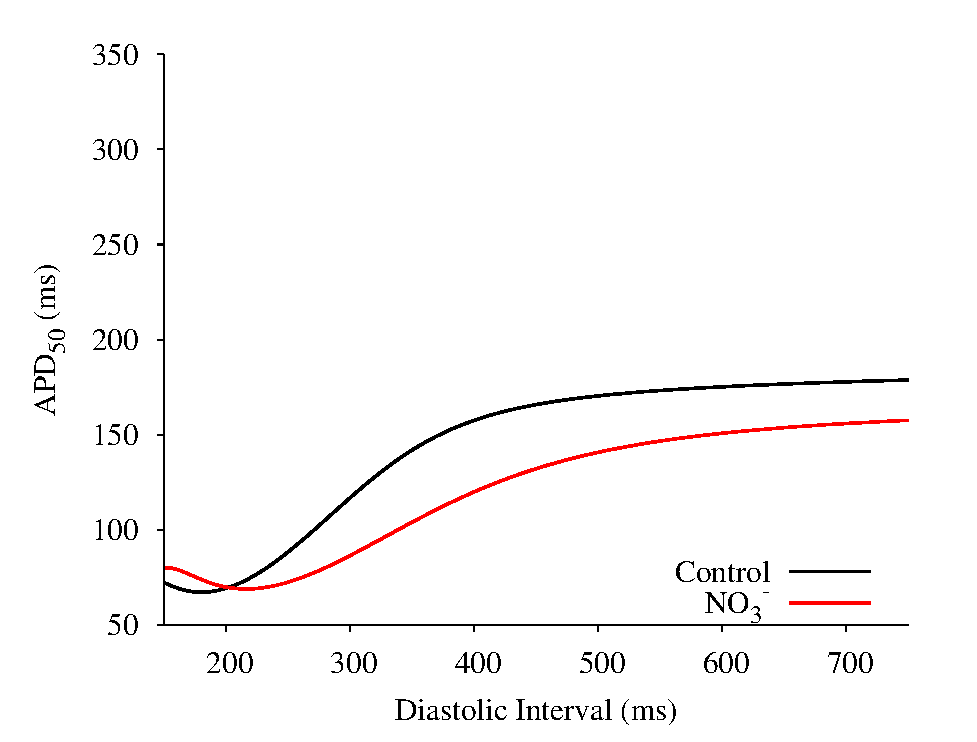
\includegraphics{figures/toolkit/anion/03_S1S2_50}
\caption[Anion Sensitive APD Restitution at 50 repolarization]{
\label{anion:apdr50} APDr curves for the CRN model in control (black) and anion
(red) cases at 50\% repolarisation.  The two variants are clearly different for
all the DI tried in the simulation, with the anion case considerably below the
control case for much of the DI tried.  The anion case also shows a reduced
slope of the restitution curve compared to the control case.  Note the
cross-over of the curves at a DI of \ms{200}.}
\end{figure}

\begin{figure}
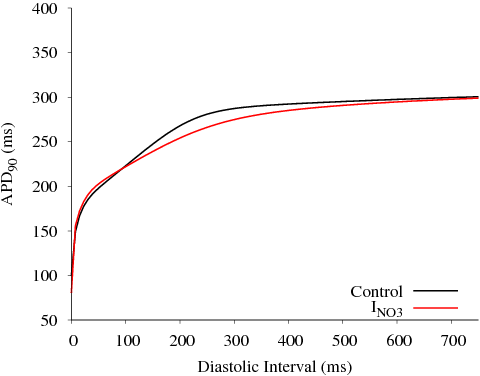
\includegraphics{figures/toolkit/anion/02_S1S2_90}
\caption[Anion Sensitive APD Restitution at 90 repolarization]{
\label{anion:apdr90} APDr curves for the CRN model in control (black) and anion
(red) cases at 90\% repolarisation.  The two variants behave the same at large
DI, but as the DI before the S2 stimulus is decreased, the anion case shows a
greater reduction in the \apd.  At short DI (below \ms{100}) the two curves
rejoin each other.}
\end{figure}

The ERP\emph{r} curves produced by the control and anion cases are shown in
figure~\ref{anion:erpr}.  In both cases the ERP\emph{r}\ curves are relatively
flat, decreasing by approximately \ms{60}\ over the \ms{700}\ range of S1
intervals considered.  The addition of the \ii{ANION}\ current changes the
behaviour of the ERP\emph{r} curve in a manner which is not simply a shift left
or right.  The control case shows a response which has a clear plateau region
which continues until an S1 interval of \ms{500}\ is reached and then a
relatively steeper decline until eliciting an AP of the appropriate magnitude
becomes impossible at an S1 interval of \ms{330}.  The anion case, by contrast,
shows a decreasing ERP over the whole range of S1 intervals considered although
it too shows its steepest slope just before eliciting a sufficiently large AP
becomes impossible, also at approximately \ms{330}.  At long S1 intervals (above
\ms{700}) the ERP\emph{r}\ is longer for the anion case before the curves cross
at \ms{600}\  and then again at \ms{450}\ with the ERP in anion at the point
where further stimulation becomes impossible almost \ms{20}\ higher than in the
control case.

\begin{figure}
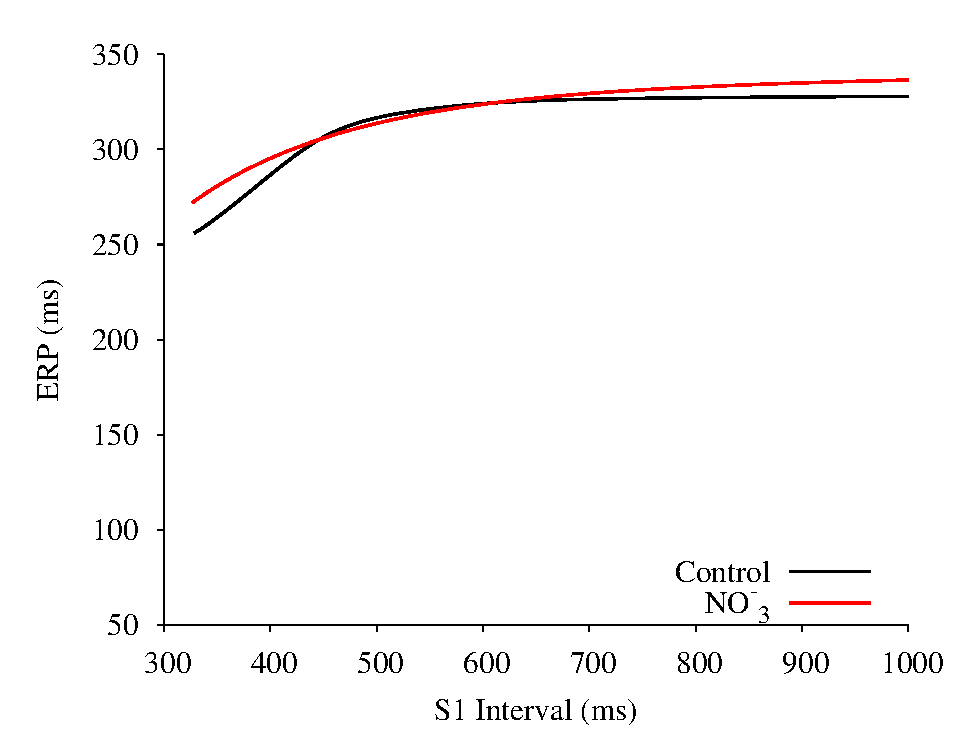
\includegraphics{figures/toolkit/anion/04_ERPR}
\caption[Anion Sensitive Effective Refractory Period Restitution]{
\label{anion:erpr} ERP\emph{r} curves for the CRN model in control (black) and anion
(red) cases.  The
addition of the \ii{ANION} current changes the behaviour of the cell from a long
and flat plateau region followed by a relatively sharp decrease into a more
constant decline.}
\end{figure}

The temporal VW increased with the addition of the anion current from
\ms{3.20} in
control to \ms{3.81}\ in anion case, a 20\% increase in the size of the region of
unidirectional conduction block.  The CV\emph{r}\ curves, shown in
figure~\ref{anion:cvr}, suggest that tissue with the anion sensitive current
shows faster CV at normal physiological stimulus intervals (corresponding to
\msrange{500}{1000}), with an average conduction velocity of
\cms{27.2}\ in anion, compared with \cms{26.9}\ in control.  As the conduction
interval is reduced below \ms{500}, the conduction velocity starts to decrease
rapidly until conduction stops at \ms{325} for anion and \ms{319} for control.
There is a brief recovery of conduction velocity visible in both cases, just
before conduction block.

\begin{figure}
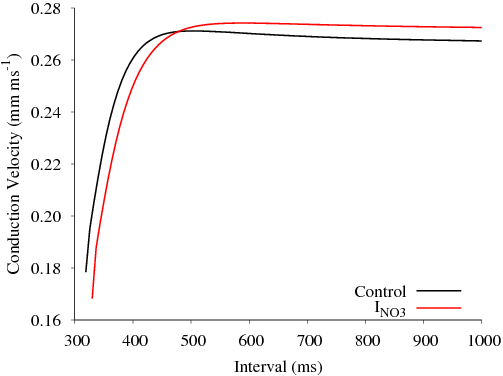
\includegraphics{figures/toolkit/anion/06_CV}
\caption[Anion Sensitive Conduction Velocity Restitution]{
\label{anion:cvr} CV\emph{r}\ curves for the CRN model in control (black) and anion
(red) cases. The CV\emph{r}\ curves are relatively flat for both cases over the range of
\msrange{500}{1000}, before they both increase rapidly in steepness until the minimum
stimulus interval is reached at approximately \ms{320} for both control and anion.
The CV is higher at longer stimulus intervals for the anion case, before it
crosses the control curve at a approximate stimulus interval of \ms{460}.}
\end{figure}

Spiral waves were induced in a square sheet.  Representative plots of the
membrane potential over the whole sheet, produced as the simulation was ongoing,
are show in figure~\ref{anion:spiral}.  Panels A i--iv show the membrane
potential for control, whilst Panels B i--iv show the membrane potential for
anion, as the simulation evolved.  The path followed by the spiral wave tip as
it meandered is shown in A,v and B,v for control and anion, respectively.  In
both cases the spiral wave starts in the centre of the tissue and then follows a
looping track around the tissue before finally it exits the tissue when it
cannot turn fast enough around its own refractory tail.  This process takes
\ms{1700} in control and \ms{2300} in anion.

\subsubsection{Discussions and Conclusions}

The effects of the inclusion of an anion sensitive current do not seem to be
that large, at least when considered on the single cell level.  This is perhaps
to be expected, as a current which did have a significant influence on the
action potential would surely have been identified sooner.  However, despite the
current's small influence on the action potential duration, it does have
significant effects on the restitution properties of the cell and on the
behaviour of cells in a tissue.

The most noticeable effect of the inclusion of \ii{ANION}\ in a cellular model
is the abbreviation of the \apd[50]\ and the accompanying reduction in the
plateau potential.  The abbreviation is due to \ii{ANION}\ acting as a
rectifying current when the membrane potential is above \mv{-45}.   Conversely,
at potentials below \mv{-45}\ \ii{ANION}\ acts to depolarize the cell, leading
to the slightly elevated resting membrane potential observed between action
potentials.  This difference in effect is what leads to the interesting
behaviours observed in cells with \ii{ANION}.

The \apdr[50]\ and \apdr\ curves show that \ii{ANION} has a rate dependent
effect.  Both curves are flattened in the cells which include \ii{ANION}\, but
this flattening is not uniform over the range of S2 intervals considered.
\ii{ANION}\ has a simple exponential dependence on the membrane potential and no
gating variables however, so it is not \ii{ANION}\ which causes this rate
dependence directly.  Instead, we must look to the currents active within the
plateau region of the action potential.  \ii{CaL}\ is the principle current
responsible for the plateau region of the action potential and unlike \ii{ANION}
it has both an activation gate, $d$, and an inactivation gate, $f$.  The $d$\
gate is not as interesting as the $f$\ gate, as its time-course is not affected
by the presence of \ii{ANION}, although its activation during the plateau region
is reduced.  Conversely, the $f$\ gate in \ii{ANION} cells never inactivates as
completely as it does in the control simulations which lack the current.

Considering next the 1D strand results, both the CV\emph{r} and threshold of
excitation data continue the story of a rate dependent influence.  At a long
stimulus interval, the increased excitability of the anion cells leads to a
higher conduction velocity.  The increased excitability at long stimulus
interval is due to the inward nature of the current in the very first stages of
the action potential.  This increased excitability allows the cells with
\ii{ANION}\ to conduct excitation faster until, at stimulus intervals of below
\ms{500}\ control cells start to conduct faster.  At this stimulus interval, the
threshold of excitation is still lower for the anion case, so another factor is
responsible for the reduction in conduction velocity.  The excitability of the
cell is an important influence on the conduction velocity, but it is not the
only factor.  Another major factor is the upstroke velocity which is principally
governed by the fast sodium current, \ii{Na}.  This is partially inactivated by
the elevated resting potential in the anion case, which also reduces the rate of
recovery of the inactivation variables.  When the test stimulus is delivered
after a reduced conduction interval in the anion case \ii{Na}\ does not open as
fully, slowing the upstroke and thus leading to a reduced conduction velocity at
short stimulus intervals, compared with the control case.  The increase in the
vulnerability window appears to be quite significant, an extra 20\% of the size
of the vulnerability window in tissue without \ii{ANION}.  Both the reduced
vulnerability window and the reduced conduction velocity at short pacing
intervals suggests that the addition of \ii{ANION} may be pro-arrhythmogenic.
The increased vulnerability window has an obvious influence on the genesis of
re-entrant excitation---A larger vulnerability window increases the chance of a
premature excitation interrupting the normal function of the heart.  The
influence of conduction velocity on re-entrant excitation is subtler, but a
reduced conduction velocity reduces the wavelength of the excitation wave.  This
allows a greater number of excitation waves to persist in the same area of
tissue, reducing the likelihood of a re-entrant excitation self-terminating.

Finally, considering the results from the sheet model of the tissue which was
used to investigate the lifespan of induced spiral wave re-entry, we can see our
hypothesis from the 1D strand results is born out.  A revolving spiral wave
typically rotates at a higher frequency than the normal excitation rate of
cardiac tissue.  The excitation waves in the 2D sheet are therefore operating in
the short stimulus interval regime.  Cells which contain \ii{ANION}\ have a
slower conduction velocity in this regime and so the spiral wave can be
sustained for longer due to it's shorter wavelength.  However, the reduction in
wavelength is not so severe as to create a stable mother rotor, as been observed
in studies of pathological conditions.

\subsection{Atrial Fibrillation Induced Remodelling And Heterogeneity}

\subsubsection{Introduction}

The human atria consists of several tissue types each with distinct
electrophysiological properties.  It has previously been shown that
inhomogeneity in tissues can lead to re-entrant activity
\cite{Bernus2005, Coronel1992, Kumagai1997}.  There is also experimental
data available on the ion channel remodelling due to atrial
fibrillation induced remodelling (AFER) during chronic atrial
fibrillation (AF) on human atrial cells~\cite{Bosch1999,Workman2001}.

In this study, we quantified the changes in electrophysiological
behavior in cell and 1D homogeneous models under AFER compared to control
conditions.  Further, re-entrant waves in 2D electrically homogeneous
and electrically heterogeneous sheets were studied.

\subsubsection{Methods}

The human atrial action potential (AP) model by Courtemanche et
al.\cite{crn98} was used in this study.  Modifications were
incorporated to reproduce the differing APs of the different atrial cell
types~\cite{Seemann2006}.  This produced distinct APs for the
crista terminalis (CT), pectinate muscles (PM), atrio-ventricular ring
bundle and the Bachmann bundle.  Atrial myocyte (AM) cells were modelled
by the original CRN model.

The data for AFER were taken from experiments by Bosch et
al.~\cite{Bosch1999} and Workman et al.~\cite{Workman2001}, representing
the changes in ion channels in patients after one month (AF1)
and up to six months (AF2) of chronic AF, respectively.  The
modifications to the cellular electrophysiology were described in
Kharche et al.~\cite{Kharche2007}.

The effects of AFER were quantified through a variety of measures.  The
\apdr\ and the \apdr[50]\ were calculated
as described in .  There were 9 S1 stimuli at a frequency of
\unit{1}{Hz}, followed by a varying DI.  The ERP\emph{r}
was calculated as described previously, with 7 S1 delivered at the given pacing
rate and then a final S2 stimulus was used to determine the ERP after Workman et
al.~\cite{Workman2001}.  The VW and the CV\emph{r} were determined for control,
AF1 and AF2 conditions, for each of the three atrial cell types classified by
Seemann et al.. There were therefore nine 1D strand models tested.  The strand
models were each 200 nodes long, with a spatial resolution of \mm{0.1}.  The
diffusion constant used for all simulations was set to
$0.03125\,\text{mm}^{\text{2}}\,\text{ms}^{\text{-1}}$~\cite{Biktasheva2005},
giving a solitary wave conduction velocity of
$0.267\,\text{mm}\,\text{ms}^{\text{-1}}$\ in control atrial tissue.  In all 1D
strand simulations there was 1 S1 pulse and one S2 pulse.  This pulse was
applied over 4 nodes (\unit{0.4}{mm}), had duration \ms{2} and magnitude
\unit{10}{nS}.

Further, a 2D electrically heterogeneous sheet model was developed based on a
laboratory photograph of the right atrium.  The photograph was digitized at a
spatial resolution of \mm{0.1}. The model developed by segmenting areas of the
tissue into AM, PM and CT tissue types.  The complete model had an approximate size of
$130\times100\,\text{mm}$ and consisted of approximately 1 million active cell nodes.  The
simulations were performed with all cells under control, AF1 and AF2 conditions,
with the conditions applied uniformly to the tissue.  All 2D sheet simulations
were performed with the space step of \mm{0.1} and a time step of \ms{0.05}.

\subsubsection{Results}

Simulations were performed for all three cases: control, AF1 and AF2.
However the results for AF1 and AF2 were qualitatively similar, although
AF1 showed a much more profound effect on \apd\ reduction.

Incorporating the heterogeneity and AFER data causes significant
differences in \apd\ to manifest, as shown in Figure~\ref{fig:apdr}. The
effects of AFER are not uniform across the different cell types of the
atrium and it increases the difference in \apd\ between normal atrial
myocytes and the CT cells, increasing from \ms{20.1} in control to \ms{28.1}
in AF1 and \ms{33.4} in AF2.

The APD\emph{r} curves, shown in Figure~\ref{fig:apdr}, are flatter over much
of the range of diastolic intervals for AF1 and AF2 as compared to
control.  However, the maximal slopes
of the APDr curves for CT cells are higher for AF1, 5.3, and AF2, 2.8,
compared with 2.1 in control.  The difference in the maximal slopes in
different tissue types is increased, with CT having a larger maximal
slope in all cases.  In the control tissue, the difference in maximal
slopes was 0.1, compared with 0.4 in AF1 and 0.5 in AF2 tissue.

\begin{figure}[tb]
\centering
%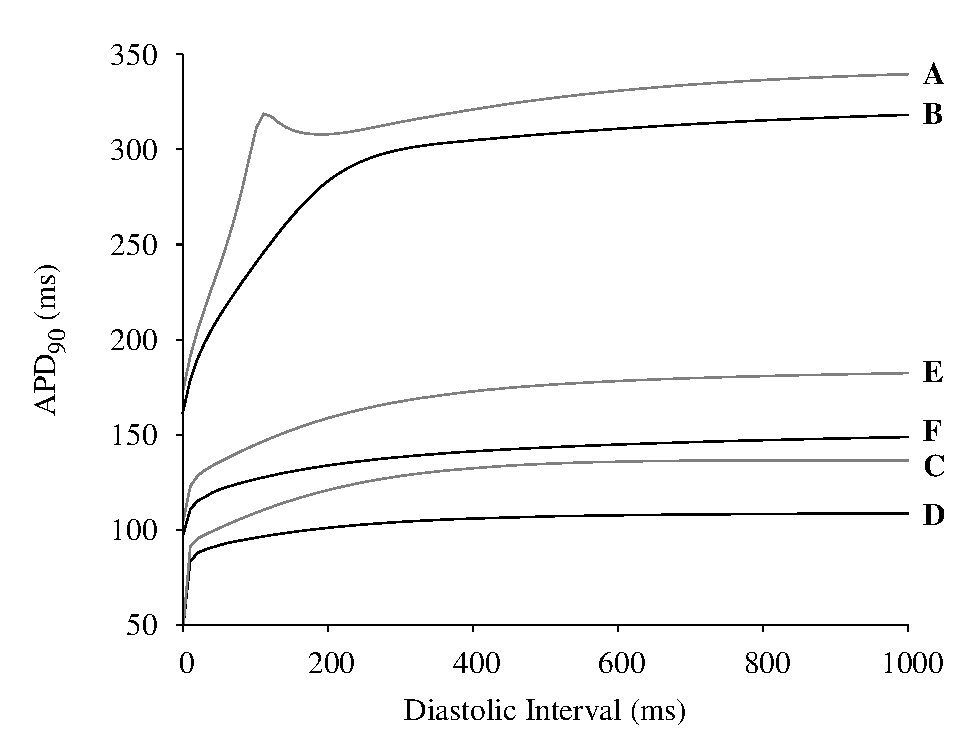
\includegraphics{figures/2_apdr}
\caption{APDr curves for control CT (A), control AM/PM (B), AF1 CT (C),
AF1 AM/PM (D), AF2 CT (E), AF2 AM/PM (F). In all cases the CT action
potentials are above the AM/PM action potentials over the whole of the
range considered.}
\label{fig:apdr}
\end{figure}

In AF tissue, the ERP\emph{r} was flattened for all tissue types compared with
the control cells, as shown in Figure~\ref{fig:erpr}.  The curves also extended
to lower BCLs for AF tissue, indicating that it was possible to excite AF tissue
successfully at a higher rate than was possible in control tissue.
Heterogeneity in ERP\emph{r} was largely unaffected by AF.

\begin{figure}[tb]
\centering
%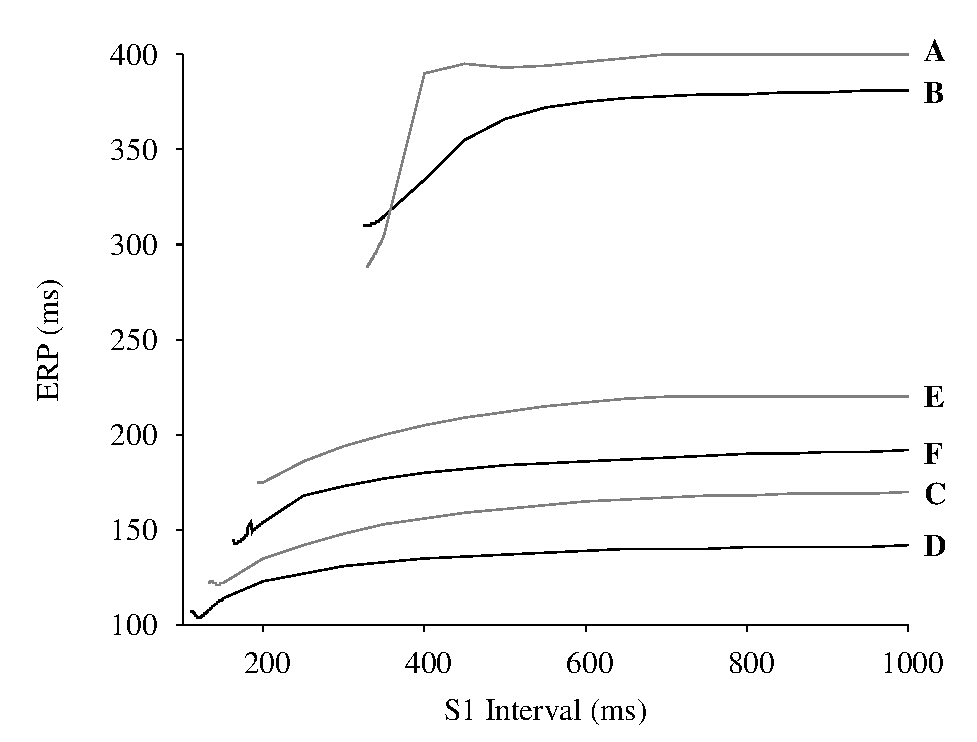
\includegraphics{figures/3_erpr}
\caption{ERPr curves for control CT (A), control AM/PM (B), AF1 CT (C),
AF1 AM/PM (D), AF2 CT (E), AF2 AM/PM (F).  Both AF1 and AF2 have a
significantly reduced ERPr over the whole range considered, with AF1
having a lower ERP then AF2.  In addition, AF1 and AF2 cells are still
excitable after pacing at \ms{100} shorter BCL.}
\label{fig:erpr}
\end{figure}

Conduction velocity, shown in Figure~\ref{fig:cvr}, was slowed by AF,
reducing the solitary wave velocity from $0.27\,\text{mm}\,\text{ms}^{\text{-1}}$\ in
control to $0.25\,\text{mm}\,\text{ms}^{\text{-1}}$\ in AF1 and
$0.26\,\text{mm}\,\text{ms}^{\text{-1}}$\ in
AF2.  Maximal pacing rate increased from the control value of \unit{198}{bpm} to
\unit{421}{bpm} in AF1 strands and \unit{315}{bpm} in AF2 strands.

The VW was reduced by AF, but in all cell types the reduction was small.
The control value of \ms{16.6} was reduced to \ms{14.2} in AF1 and \ms{14.7}
in AF2 for AM and PM cell types.  The reduction in VW for CT cells was
even smaller, from \ms{15.1} in control to \ms{14.5} and \ms{14.4} in AF1 and
AF2, respectively.

\begin{figure}[tb]
\centering
%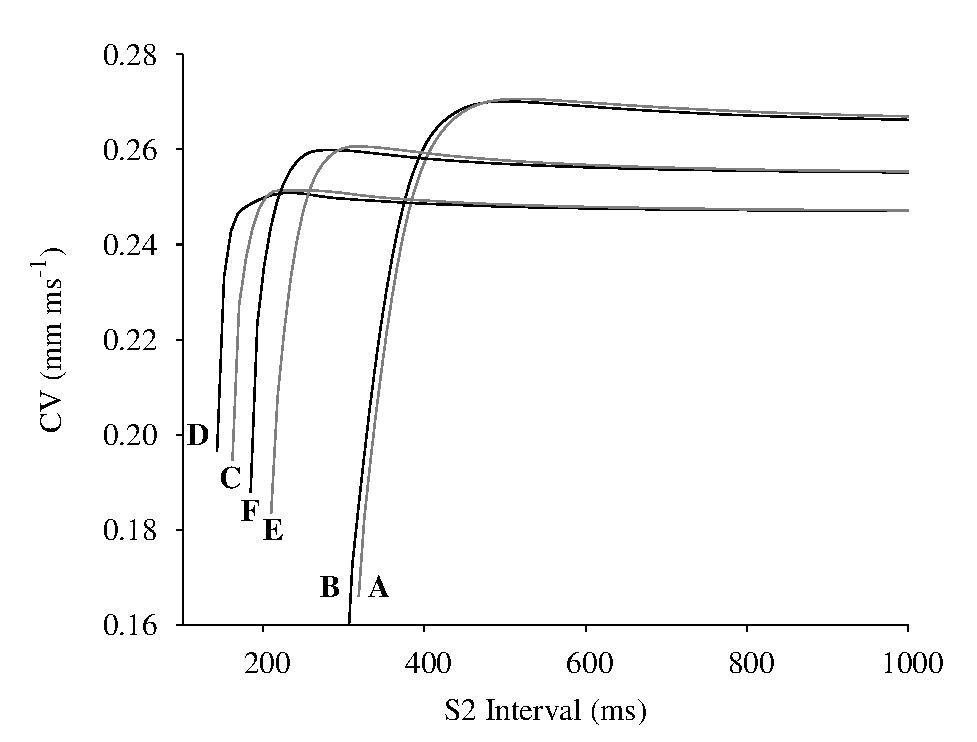
\includegraphics{figures/4_cvr}
\caption{CVr curves for control CT (A), control AM/PM (B), AF1 CT (C),
AF1 AM/PM (D), AF2 CT (E), AF2 AM/PM (F).  In each of the conditions,
the CT cells showed a higher CV at long (1000~ms) S2 intervals, but AM
and PM cells allow faster conduction at shorter S2 intervals.  The AF
cases show reduced CV compared to the control and support a higher
pacing rate via reduced minimum interval.}
\label{fig:cvr}
\end{figure}

Simulations over the 2D geometry examined the lifetime and behavior of
spiral waves in the presence and absence of electrical heterogeneity.
As can be seen in Figure~\ref{fig:plots}, panels Ai and Bi, re-entrant
activity self-terminated in both homogeneous and heterogeneous cases
when due to spiral wave meander over a large tissue region, it
exits the tissue.  Self-termination was much more rapid in the
electrically heterogeneous case, taking \unit{1.31}{s}, compared with
\unit{3.20}{s} in
the homogeneous case.

Conversely, under AF conditions the re-entry persisted after it was
induced for the whole period of the simulation, a lifespan of over \unit{5}{s}.
Under electrically homogeneous conditions, panels Aii and Aiii show a
stable mother rotor rotating anti-clockwise in the tissue.  But in
heterogeneous conditions, as shown in panels Bii and Biii, a similar
mother rotor to the homogeneous cases is visible towards the right of
each frame.  On the left of the frames, the rotor breaks up into
multiple fibrillatory wavelets on the border of the heterogeneous
regions, forming a complex and chaotic pattern of excitation.

\begin{figure*}[t]
\centering
%\includegraphics{figures/figure4}
\caption{Simulation of re-entry in 2D sheets of electrically homogeneous
(A) and electrically heterogeneous (B) sheets.  Columns show
representative frames after initiation of re-entry at t = 0.  Panels i
show data under control conditions, panels ii under AF1 conditions and
panels iii under AF2 conditions.  Re-entry self-terminated under control
conditions in both homogeneous (Ai) and heterogeneous (Bi).  Under AF
conditions, re-entry becomes a sustained mother rotor in
electrically homogeneous conditions (Aii, Aiii).  However, under
electrically heterogeneous conditions AF causes re-entry to degenerate
into erratic propagations on the borders of the heterogeneity (Bii,
Biii).}
\label{fig:plots}
\end{figure*}

\subsubsection{Discussion and conclusions}

AFER induces significant changes in the cellular electrophysiology that
appear to affect rate dependent electrical activities.  It helps to
sustain re-entry, providing evidence to substantiate the hypothesis of
``AF begets AF''.

Considering first the single cell results, one of the most obvious
effects is the striking reduction in the \apd\ and repolarization
properties.  AFER abbreviated \apd\ in AM cells by 66~\% in AF1 and
53~\% in AF2.  Other work has already suggested why the increases shown
in the maximal slope of the APDr can be
pro-arrhythmic~\cite{ByungSoo2002}, as can the reduced
ERP~\cite{Xie2002}.  Our study suggested that reduction is not uniform
across all cell types, which leads to an augmented heterogeneity.

The 1D strand results for the CV tell a similar story.  AFER tissue
forms a much better substrate for arrhythmic activity, supporting both a
much higher maximal pacing rate and in addition, the reduction in
conduction wavelength, to below half the control values. This allows a
greater number of excitation waves to exist in the tissue at any one
time.

The 2D simulations in the realistic sheet show a marked difference in
re-entrant behavior between homogeneous and heterogeneous simulations.
The homogeneous sheets show self-termination of re-entry in control
tissue, whilst the reduced ERP and conduction wavelength allow the rotor
to remain stable and persist for the duration of the simulation in AFER
condtions.  The heterogeneous sheet simulations, show spiral wave
breakup, as observed in real tissue \cite{Kumagai1997}, in both control
and AF simulations, possibly due to elevated plateau potentials and
increased refractory period of the CT cells.  Self-termination is still
observed in control simulations and is more rapid than in homogeneous
tissue.

It is still unclear about the pro- or anti-arrhythmogenic effects of
electrical heterogeneity in the human atria.  Self-termination is more
rapid in the heterogeneous tissue for the control case, but despite AFER
increasing the heterogeneity between tissue types, it doesn't lead to
self termination of the re-entry.  In fact, it leads to breakup of the
spiral wave in the region of the heterogeneity, leading to a region of
erratic propagations, as has been seen in experiment~\cite{Kumagai1997}.
Further study, in both 3D geometries and physiological experiments,
would be needed to elucidate the true effects of the heterogeneity.



   \chapter{Modelling the Whole Atrium}

In the previous chapter a modelling library suitable for simulation of single
cell and over 1D and 2D models of cardiac tissue was developed.
Single cell models are the base on which 1D and 2D models stand and 1D and 2D
models provide valuable insight into the behaviours of cardiac tissue in health
and disease.
It does not need to be said that the atrium is not 1D or 2D construct but is
instead a complex 3D structure.
This complexity can be seen internally, in that the atrium is comprised of several
separate tissue types with distinct electrophysiological behaviours and has
regions of differing conductivity.
It can also be seen in the gross physical structure, the atrium has a complex
topology with both holes for the venous and arterial openings, as well as
openings for the valves.
The simpler, often idealized, models constructed in the previous chapter
ignore (and in many cases, are incapable of showing) many of these complexities.
To provide insight into the atrium function on the whole organ level we must
therefore simulate the atrium as an organ.
A 3D model of the atrium requires a representation of the atrial geometry to
provide the topology of the atrium.
To model complexities with sufficient accuracy models of the
electrophysiologically distinct tissue types are also required as are
descriptions of the complex conductivities.


\section{Atrial Geometry}
\label{atrium:sec:geometry}

The atrial geometry used in the simulation studies presented here was based on
the visible human project female dataset.  The visible human dataset was
created from a pair of cadavers, set into wax and sliced into \mm{1}\ and
\mm{0.33}\ for the male and female bodies, respectively.  The geometric model
used here was extracted from the female dataset and so has a resolution of
\mm{0.33}.  The extracted geometry is segmented into different tissue types,
with distinct classifications for left and right atrium, the pectinate muscles,
the crista terminalis, the Bachmann bundle and the sino-atrial node, as shown in
figure \ref{atrium:geometry}.  The geometry has been used in numerous previous
simulation studies.  It was discretised via a finite differences approach, which
allows the whole atrium to be embedded in a block of $298\times269\times235$
nodes.  This gives it a total size of approximately 19 million total nodes,
although only approximately 1.6 million of those nodes correspond to excitable
cells.  The geometry also has simple fibre orientation in the pectinate muscles,
crista terminalis and Bachmann bundle.  The fibres are considered to always run
parallel to the local axis of the tissue bundle, as determined by principle
component analysis~\cite{Seemann2006}.

\section{Simulation Methods}
\label{atrium:sec:model}

\subsection{Atrial Model}

The electrical activity at each of the nodes was described by the equations of
the Courtemanche--Ramirez--Nattel (CRN) of the human atrial
myocyte~\cite{crn98}.  This model, as previously described, is a second
generation model. It has 21 state parameters, representing ionic gating activations
and inactivations and intracellular concentrations of ionic species.  In the
model, the total current, \ii{ion} is made up of the contributions of numerous
channels
\begin{equation}
\label{atrium:crn}
\ii{ion} = \ii{Na} + \ii{K1} + \ii{to} + \ii{Kur} + \ii{Ks} + \ii{Kr} +
\ii{Ca,L} + \ii{p,Ca} + \ii{NaK} + \ii{NaCa} + \ii{b,Na} + \ii{b,Ca}
\end{equation}
where \ii{Na}, \ii{K1}, \ii{to}, \ii{Kur}, \ii{Ks}, \ii{Kr}, \ii{Ca,L},
\ii{p,Ca}, \ii{b,Na} and \ii{b,Ca}\ represent ionic currents and \ii{NaK}\ and
\ii{NaCa}\ are ion exchangers.  As a second generation model, the CRN model also
has a detailed calcium handling system which can influence the action potential
via its influence on the intracellular calcium concentration.

In some atrial simulations it was desirable to incorporate details of
electrophysiological heterogeneity to represent the difference in electrical
behaviour between atrial myocytes and the other cellular types present in the
geometry, the pectinate muscles and crista terminalis.  The parameters used for
heterogeneity were based on measurements taken by Feng et al.~\cite{feng1998}
of the canine atrium.  These were converted to parameters for the CRN model by
Seemann et al.~\cite{Seemann2004} and have been used in several simulation
studies~\cite{Seemann2006,Stott2008}.  They are shown in
table~\ref{atrium:het_params}.

\subsection{Monodomain Equation}

To simulate the propagation of electrical activity over the finite difference
geometry previously described, the mono-domain equation is used to describe the
changes in $V$ in time, $t$, the trans-membrane voltage.
\begin{equation}
\label{atrium:monodomain}
\frac{\partial V}{\partial t} = \nabla\cdot D \nabla V - \frac{\ii{ion}}{C_{m}}
\end{equation}
where $D$ is a tensor representing the diffusivity of electrical potential, \ii{ion} is described by the
CRN model (\ref{atrium:crn}), $C_{m}$ is the membrane capacitance and all other
symbols have their usual meanings.  Equation (\ref{atrium:monodomain}) is
advanced in time via the forward euler method with a timestep of \ms{0.05}.  For
simulations with isotropic conductivity between nodes a 7-node approximation of
the differential operator is used.  When anisoptropy is present, a 27-node
approximation is used.

\subsection{Tissue Anisotropy}

The heart has a complex fibrous structure (Chapter 1), and this manifests
electrically as regions which have preferential conduction directions.
The preferential conduction directions show greatly increased conduction
velocities, sometimes by a factor of up to five~\cite{}.
The fibre structure and regions of preferential conduction are generally
considered much more important for the ventricles than for the atria.
The atria, or more specifically the right atrium, do possess several structures
with a definite direction of preferential conduction.
These are the crista terminalis, responsible for rapid conduction of the
depolarization wave to the atrio-ventricular node, the pectinate muscles and the
Bachmann bundle, the preferential pathway for conduction between the atria.
To determine the influence of anisotropic conduction on the propagation of the
electrical activity, we follow a method after Panfilov and
Keener~\cite{panfilov1995}.
In this method there is a unit vector, $\mathbf{f}$, defined at every point in
the tissue which has significant fibre orientation.
This unit vector defines a set of co-ordinate axes, in which the conductivity
tensor is diagonal
\begin{equation}
\label{atrium:dtilde}
\mathbf{\tilde{D}} =
\begin{pmatrix}
D_{\parallel} & 0 & 0\\
0 & D_{\perp} & 0\\
0 & 0 & D_{\perp}
\end{pmatrix}
\end{equation}
where $D_{\parallel}$ is the diffusion constant for conduction parallel to the
preferential direction of conduction and $D_{\perp}$ is the diffusion constant
for conduction perpendicular to this direction.
In this formulation it is assumed that there is no `sheet' structure which gives
a higher conduction velocity in one direction perpendicular to the main fibre
axis.
The diffusion tensor $\mathbf{\tilde{D}}$\ will only be diagonal in the
Cartesian co-ordinate system of the heart if the direction of preferential
conduction is parallel to one of the axes.
Therefore, to find the conductivity tensor in the global co-ordinate system,
$\mathbf{D}$, we need to find two transformation matrices $\mathbf{A}$\ and
$\mathbf{A^{T}}$\ such that
\begin{equation}
\label{atrium:d}
\mathbf{D} = \mathbf{A} \mathbf{\tilde{D}} \mathbf{A^{T}}
\end{equation}
To find $\mathbf{A}$\ it is possible to write out the involved rotations
explicitly, however an alternative method~\cite{fention2005}\ uses the fact that
$\mathbf{f}$\ and the two vectors orthogonal to it, $\mathbf{g}$\ and
$\mathbf{h}$\ are eigenvectors of $\mathbf{D}$.
These have the eigenvalues of $D_{\parallel}$\ and $D_{\perp}$.
The matrix $\mathbf{A}$\ is therefore an orthogonal matrix of the form
$\mathbf{A} = \left(\mathbf{f},\mathbf{g},\mathbf{h}\right)$ and so, using
(\ref{atrium:d}) $\mathbf{D}$\ can be written as
\begin{equation}
\label{atrium:dfgh}
\mathbf{D} = D_{\parallel}\mathbf{f}\mathbf{f^{T}} +
D_{\perp}\left(\mathbf{g}\mathbf{g^{T}} + \mathbf{h}\mathbf{h^{T}}\right)
\end{equation}
Using the fact that $\mathbf{A}\mathbf{A^T} = \mathbf{I}$ it is possible to
write
\begin{equation}
\label{atrium:dwithf}
\mathbf{D} = D_{\perp}\mathbf{I} + \left(D_{\parallel}-D_{\perp}\right)\mathbf{f}\mathbf{f^{T}}
\end{equation}
where $\mathbf{I}$\ is the identity matrix, and all other symbols are as defined
previously.
The directions of preferential conduction for the atrial geometry used in the
study were described by a pair of angles $\theta$\ and $\phi$\ representing the
orientation of the unit vector $\mathbf{f}$\ at each point in spherical polar
co-ordinates.
In cells with no assigned preferential conduction direction, the components of
$\mathbf{f}$\ were set to zero, giving a diffusion tensor of
\begin{equation}
\label{atrium:dnofibre}
\mathbf{D} =
\begin{pmatrix}
D_{\perp} & 0 & 0\\
0 & D_{\perp} & 0\\
0 & 0 & D_{\perp}
\end{pmatrix}
\end{equation}
which is the diffusion tensor for isotropic conduction.

\subsection{Computational Implementation}

The atrial geometry used in these studies is quite large, consisting of almost
19 million nodes.
As noted in \ref{atrium:sec:geometry}, only approximately 1.6 million of these
nodes correspond to active tissue--less than 10\% of the total.
The electrical activity at each node is represented by the CRN model and thus
requires 21 double precision numbers to be stored, representing the state
variables of the model.
The memory requirements of the model may be significantly reduced by storing
state variables, and where anisotropy is present the diffusion tensor, only for
the active nodes.
This reduces the memory requirements for storing the state variables from
approximately \unit{2.9}{GB}\ to \unit{256}{MB}.
A further simplification may be obtained by decomposing the geometry into a
linear array, containing the 7 or 27 neighbours of the active nodes to be used
in the diffusion tensor approximation.
The geometry and state information can therefore be represented by one linear
array of cellular states, one linear array used as a `map' and optionally, one
linear array representing the components of $\mathbf{D}$.
This linear data structure is very easy to parallelize on a shared memory
system.

The parallelization was accomplished through the use of the OpenMP shared
memory parallelism library~\cite{OpenMP}.
The system was then solved on 1 node of the Horace supercomputer on a total of 8
cores.
The linear array of active nodes was divided equally between the 8 cores, with
each core solving (\ref{atrium:crn}) for all nodes its assigned section of the
array.
A snapshot of the trans-membrane potentials at each of the active node sites was
output every \ms{2.5}\ of simulated time.
Simulation of \unit{1}{s}\ of atrial activity took XXXX hours.
A parallel fraction of XXXX was attained, indicating that almost all of the
workload was effectively distributed over the 8 cores.

\section{Mutation in KCNQ1: A Simulation Study}

Atrial Fibrillation (AF) is the most common arrhythmia in the developed world.
It is a self-promoting condition, with paroxysmal AF episodes frequently
degenerating into chronic and even permanent AF.
Clinically, AF patients show an erratic and high frequency ECG.
At the cellular level, AF is characterised by an abbreviated action potential
(AP) which has no plateau phase and poor heart rate adaptability.
The mechanisms through which AF influences the heart are complex, but the
remodelling of the cellular electrophysiology is believed to contribute to
reduced ERPs and through that, favour the formation of stable, long lived
spiral waves and organ level microwavelet re-entry.
AF is often preceeded by congestive heart failure, cardiomegaly and other
structural cardiac diseases, but there are significant numbers of suffers with
no such structural defects.
There is also evidence of a genetic predisposition to AF, which is sometimes
termed Familial Atrial Fibrillation.
Several gene mutations have been causally implicated for AF, leading to AF
which manifests both with and without associated structural cardiac disorders.
The ion channels associated with the repolarisation reserve (\ii{K1}, \ii{Kr},
\ii{Ks}) are particularly important to the genesis of AF.
Alterations in functions, gating and kinetics have been implicated in both short
and long QT syndromes.
The \ii{Ks}\ channel has very slow activation kinetics which enable it to
regulate cardiac APs over a wide range of plateau voltages.
Mutations in the \ii{Ks}\ channel are common.
Several mutations in the $\alpha$-subunit, coded for by the KCNQ1 gene, of the
\ii{Ks}\ channel have been identified including both loss-of-function and
gain-of-function, leading to the SQT syndrome and to AF.
Chen et al. studied a four generation Chinese family with hereditary persistent
AF.
They identified a missense mutation at nucleotide 418 from adenine to guanine
resulting in a change from serine to glycine at position 140 (S140G mutation of
\ii{Ks}).
This missense mutation lead to a large gain-of-function which included changes
in the channel kinetics.
It has been hypothesised that these changes in the function of the \ii{Ks}\
channel in the human atrium result in abbreviations of both APD and ERP and thus
provide an appropriate substrate for the genesis of AF.

This study had two goals: To construct a computer model of the available
experimental data from Chen et al. and to then use this model to quantify the
effects of the mutation through the use of cellular, 1D, 2D and 3D models

\subsubsection{Modelling the Mutation}

This study, as in the previous chapter, uses the CRN model, developed by
Courtemanche et al.~\cite{CRN1998}\ for simulation of the human atrial action
potential.
As a biophysically detailed model with 21 state variables and numerous ion
channels it is ideal for use in mutation studies.
The CRN model has individual descriptions of several $K^{+}$\ currents.
These include the time-independent potassium current, \ii{K1}, the ultra-rapid
potassium current, \ii{Kur}, the transient outward current, \ii{to}\ and the
rapid and slow delayed rectifier currents, \ii{Kr}\ and \ii{Ks}.
The latter current is modulated by the mutation and is described in the control
CRN cell by
\begin{equation}
\label{atrium:iks_con}
\ii{Ks} = g_{Ks}x_{s}^{2}\left(V-E_{K}\right)
\end{equation}
where $g_{\tiny{Ks}}$\ is the channel conductance (\unit{0.129}{nS/pF}), $x_{s}$\ is
the activation variable and $E_{K}$\ is the $K^{+}$\ reversal potential, found
through the Nernst potential.

\subsubsection{Simulation of the S140G mutation of KCNQ1 I-V relationship}

The Chen et al.~\cite{Chen2003} study determined that the most likely cause of
familial AF was was the S140G mutation of the KCQN1 gene, which forms part of
the $\alpha$-subunit of the \ii{Ks}\ channel.
The gene was transfected into COS7 cells along with the second component of
the $\alpha$-subunit, KCNE1, in both normal (WT) and mutated type (MT).
The transfected cells were used to perform voltage clamp experiments.
The clamp protocol used is shown in Figure~\ref{atrium:iks:vc},A.
This is the experimental protocol used by Chen et al.~\cite{Chen2003}.
The cell was held at a holding potential of \mv{80} for \unit{0.5}{s}\ before
being held at \mv{10}\ steps between \mv{-130}\ to \mv{50}\ for \unit{3}{s}.
The voltage steps were followed by a \mv{-40}\ holding potential, applied for
\unit{1}{s}.
The values of \ii{Ks} at the end of the step voltages were plotted against the
step voltages to determine  I-V relationships for WT
and MT cells, shown in Figure~\ref{atrium:iks:vc},B (points with errors) and
current traces, shown in Figure~\ref{atrium:iks:vc},C and D for WT and MT,
respectively.

\begin{figure}
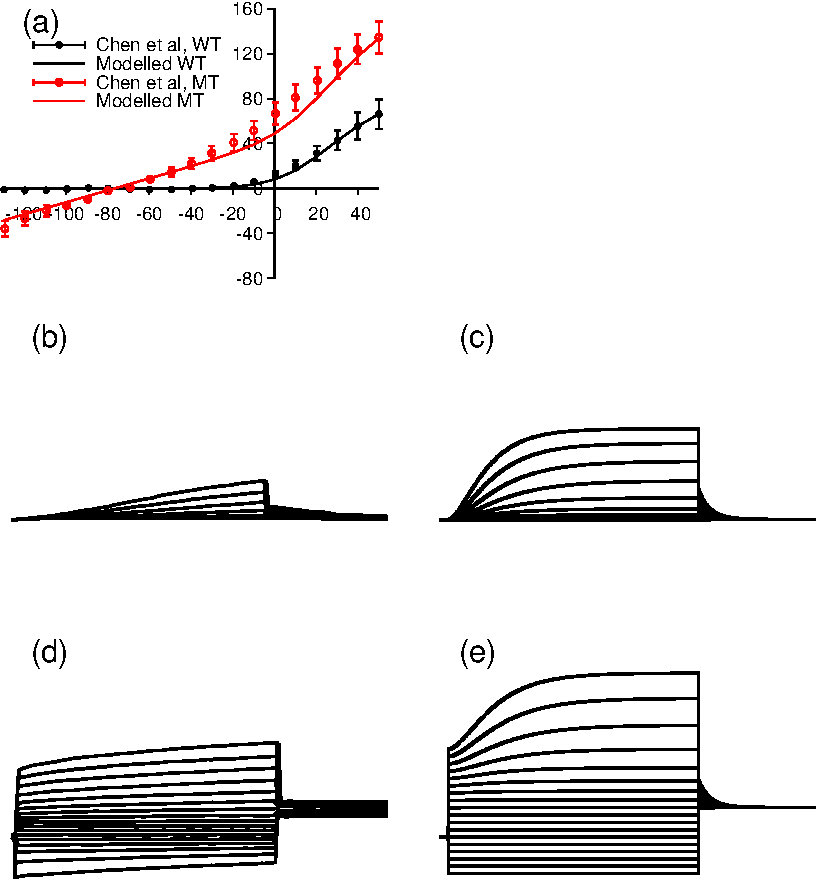
\includegraphics{figures/atrium/iks/figures/01_IV}
\caption[KCNQ1 mutation in IKs, experimental data]{
\label{atrium:iks:vc}
\textbf{A} Voltage clamp protocol used by Chen et al.~\cite{Chen2003}.
\textbf{B} Experimental WT (black, closed circles) and MT (red, open circles)
I-V relationships recorded by Chen et al.  Simulated I-V curves for WT (black
lines) and MT (red lines).  Modelled curves are scaled to experimental points
based on the WT current density at \mv{50}.
\textbf{C} Experimental current traces for WT.
\textbf{D} Simulated current traces for WT.
\textbf{E} Experimental current traces for MT.  Note the instantaneous
activation, and the significant inward current at negative clamp potentials.
\textbf{F} Simulated current traces for MT.
}
\end{figure}

The I-V relationship shows that the mutation causes a gain-of-function across
all the clamp potentials.
It also reveals that the mutation appears to cause an inward current at negative
potentials.
The current traces suggest a drastic change in the kinetics of the \ii{Ks}\
channel with a significant component of the current being activated immediately.
The addition of a leakage component to (\ref{atrium:iks_con}) allowed simulation
of \ii{Ks}\ characteristics which closely matched the experimental data.
Under MT conditions, the new total current \iip{Ks}\ was described by
\begin{equation}
\label{atrium:iks_mut}
\iip{Ks} = \ii{Ks} + \varphi g_{Ks}x\left(V-E_{rev}\right)
\end{equation}
where \ii{Ks}\ is (\ref{atrium:iks_con}), $\varphi$\ is a multiplicative parameter
from with values between 0 and 1, $g_{Ks}$ is as in (\ref{atrium:iks_con}) and
$E_{rev}$\ is the reversal potential of the leakage component.
The reversal potential was estimated from the experimental I-V relationships to be
\mv{-76.3}.
The inclusion of the $\varphi$\ parameter allowed the simulation of several
intermediate mutant states, representative of a heterozygous mutation.
Setting $\varphi = 1$\ and following the voltage clamp protocol shown in panel A
of Figure~\ref{atrium:iks:vc}\ the I-V relationship of \ii{Ks}\ was simulated to
provide a good match to experimental data shown as the lines in panel B of
Figure~\ref{atrium:iks:vc}.
Also shown are the simulated current traces elicited by the voltage clamp
protocol in panels D and F.
The non-gated leakage component of \iip{Ks}\ sufficiently accounts for the
changed current density and kinetics.

\subsubsection{Simulation Protocols}

To assess the effects of the mutation on human atrial myocytes, cellular models
including the modified \iip{Ks}\ described by (\ref{atrium:iks_mut}) were used
in a number of simulation protocols, as described in Chapter 2.
Initially the \apd\ was evaluated under conditions corresponding to $\varphi =
0$\ (WT) and $\varphi = 1$\ (MT).
Under such conditions, the induced \apd\ shortening was found to result in
un-physiological \apd\ values, shown in Figure \ref{atrium:iks:apd}.
Therefore a pair of heterozygous cases, corresponding to $\varphi = 0.10$\
(HT10) and $\varphi = 0.25$\ (HT25) were created and used in the evaluation of
the mutation's effects.

Using the models and protocols described in Chapter 2 the \apdr, ERP\emph{r}, VW,
CV\emph{r}, SVW and the dynamic behaviours of spiral waves were evaluated for
the WT, HT10 and HT25 cases.
For the 3D simulations, the model described in Sections
\ref{atrium:sec:geometry}\ and \ref{atrium:sec:model}\ was used.
Since the intention was just to investigate the influence of the mutation, the
model was used without tissue anisotropy.
The mutation was applied homogeneously with the electrical activity at all
nodes described by either the WT or HT10 cells.
An atrial model of nodes described by HT25 cells did support stable conduction
and so it was not used in the 3D studies.
There was no heterogeneity introduced to account for the differing cell types
present in the human atrium.
To examine the behaviour of scroll waves under WT and HT10 conditions a protocol
analogous to the wave-break protocol described for 2D sheets of tissue was
used~\cite{Kharche2007}.
The protocol is illustrated in Figure~\ref{atrium:iks:scroll_init}.
\begin{figure}
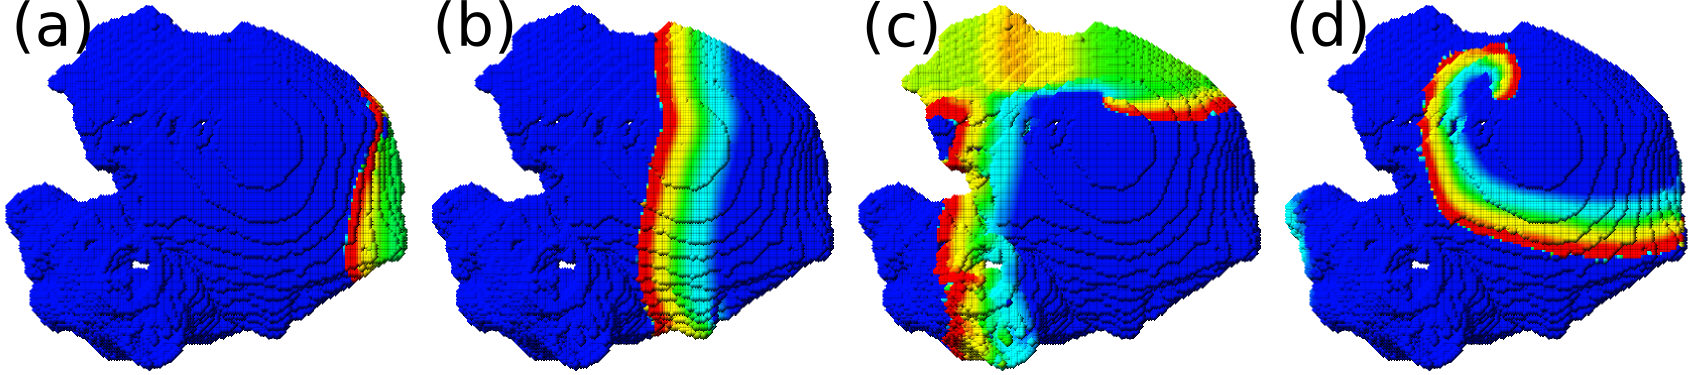
\includegraphics{figures/atrium/iks/scrollhowto}
\caption[Initiating a Scroll Wave]{
\label{atrium:iks:scroll_init}
Stimulus protocol used to initiate a scroll wave.
\textbf{A} One extreme of the atrial model is stimulated
\textbf{B} The excitation is allowed to propagate
\textbf{C} An S2 stimulus is delivered by clamping a section of the tissue, here
the lower quarter.
\textbf{D} A scroll wave begins on the wall of the right atrium.
}
\end{figure}
First, a small number of cells are simulated at one extreme of the atrial model.
The excitation is allowed to propagate through the model until the S2 stimulus
is delivered.
The S2 stimulus is delivered via briefly clamping a section of the atrial model to
\mv{50}\ and then releasing the clamp.
A correctly timed S2 stimulus results in a scroll wave on the wall of the right
atrium.
After initiation, the models were simulated until activity ceased or until
\unit{6}{s}\ of simulated time had elapsed.

\subsubsection{Changes in \apd\ due to S140G mutation}

The effect of an increase in the leakage current parameter were investigated.
This was done using the standard \apd\ protocol and varying $\varphi$\ between
0 and 1.
Variation in \apd\ as $\varphi$\ is altered is shown in
Figure~\ref{atrium:iks:aps},A.
Representative APs are shown in Figure~\ref{atrium:iks:aps},B.
The \apd\ under Control conditions (WT) was seen to be \ms{312.0}.
Progressive mutation decreased the \apd\ to \ms{150.5}\ in HT10 case and
\ms{79.3}\ in HT25 case.
Under homozygous conditions, $\varphi = 1$\, the \apd\ was seen to be \ms{22.4}.
Figure~\ref{atrium:iks:aps},B shows the inclusion of the mutant channel causes
the changes in morphology associated with none of the mutant types having a
plateau region.
Inclusion of the mutant channel decreased the upstroke velocity of the AP from
\unit{217.1}{V/s}\ in WT, to \unit{214.0}{V/s}\ in HT10 and \unit{208.6}{V/s}\
in HT25.
The upstroke velocity in the homozygous case was \unit{192.0}{V/s}.

\subsubsection{\apdr\, ERP\emph{r}, CV\emph{r} and VW}

Figure~\ref{atrium:iks:apdretal},A shows the current profiles of \ii{Ks} over the course of
an AP which correspond to the AP traces shown in Figure~\ref{atrium:iks:aps},B.
\ii{Ks}\ is seen to increase considerably in both the HT10 and HT25 cases
compared with the WT case.
The leak also changes the morphology of the current profile to one showing
almost instant activation in HT10 and HT25 cases, compared to the slow
activation in WT.
The \apdr\, Figure~\ref{atrium:iks:apdretal},B, reflects the decreased \apd\ with
the restitution curves considerably flattened for both the mutant cases.
The maximal slopes of the \apdr\ were measured to be 1.9, 0.78 and 0.56 in cases
WT, HT10 and HT25 respectively.
The ERP\emph{r}\ curves, Figure~\ref{atrium:iks:apdretal},C, also reflect the
reduced \apd\.
At an S1 interval of \ms{1000}\ the ERP was found to be \ms{XXXX}\ in WT,
\ms{XXXX} in HT10 and \ms{XXXX} in HT25.
In addition, the mutant cases supported excitation at much lower S1 intervals
(or higher pacing rate) compared to the control case.
The minimum S1 interval sustained during the ERP\emph{r}\ calculations was
\ms{XXXX}\ in WT, \ms{XXXX} in HT10 and \ms{XXXX} in HT25.
The solitary wave CV was not altered considerably by the mutation (\cms{26.7}\
in WT c.f. \cms{27.0} in HT25).
The CV\emph{r}\, Figure~\ref{atrium:iks:apdretal},D, curves confirm the findings
of the ERP\emph{r}\ calculations, that the mutant case supports successful
excitation after a considerably reduced S2 interval.
The minimum S2 interval which still allowed the test stimulus to propagate was
found to be \ms{318.9}\ in WT, \ms{181.2}\ in HT10 and \ms{120.4}\ in HT25.
Vulnerability to premature excitation was relatively unaffected by the mutation,
having a value of approximately \ms{XXXX} in all cases.

   \chapter{The Body Surface Potential}
\label{chapter:bsp}

Modelling the atrium itself can provide valuable insight into the effects and
mechanisms of drugs, diseases and inherited conditions as discussed in Chapters 2 and 3.
These simulation studies directly compute the electrical potentials generated by the heart.
However, such measurements are not available to physicians without the
insertion of a catheter electrode or other, more involved, surgical procedures.
Instead they must rely on external tools such as the echocardiogram and the
electrocardiogram (ECG).
To reproduce the ECG with mathematical models, it is necessary to solve the forward problem.

\section{The Forward Problem}

As was noted earlier ($\S$\ref{sec:intro:forward:numerical}) solving the forward
problem involves solving Poisson's equation in the body.
In an infinite homogeneous conducting medium, a solution to Poisson's equation
for the field at any given point, $\phi$, is~\cite{Plonsey1989}
\begin{equation}
\label{eqn:bsp:infinite}
\phi = \frac{1}{4 \pi \sigma} \int \frac{- \nabla \cdot
\mathbf{J}^{i} }{r} dv
\end{equation}
where $r$ is the (scalar) distance from the elemental volume $dv$ to the point at
which the field is being evaluated.
This is shown in figure~\ref{fig:bsp:vectors}.
The distance $r$ is the magnitude of the vector $\mathbf{r'}-\mathbf{r}$.


\begin{figure}
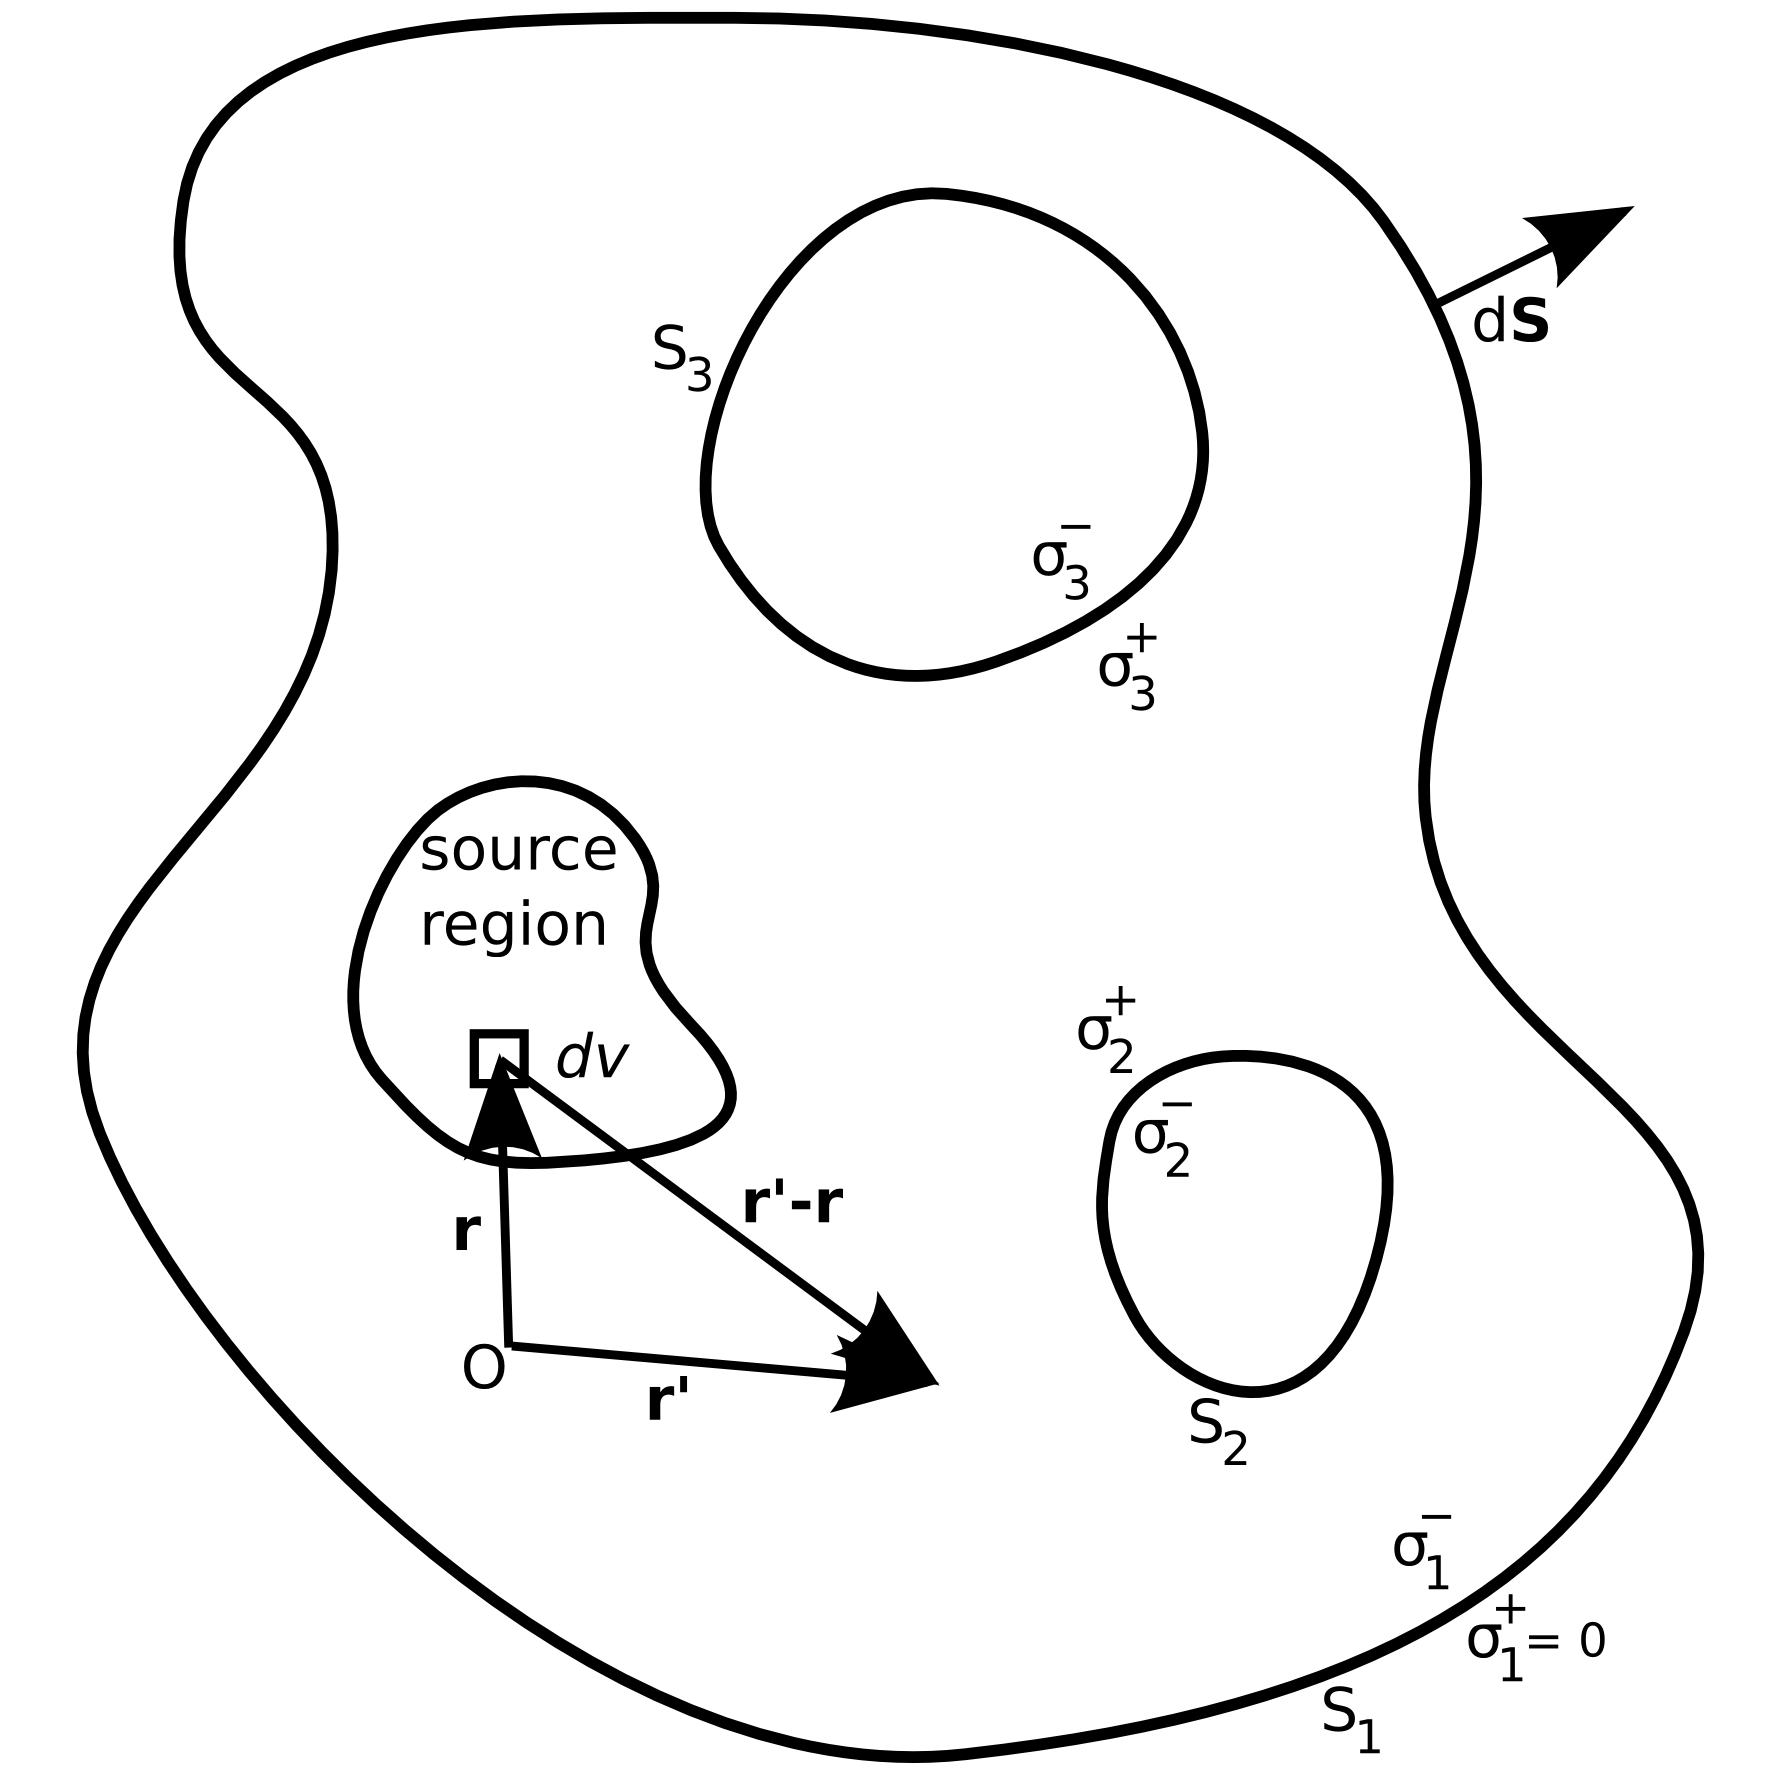
\includegraphics{figures/bsp/bsp_vectors}
\caption[Diagram of the vectors and surfaces involved in the BEM]{
\label{fig:bsp:vectors}
Vectors and surfaces involved in the boundary element method.
The origin is at point $O$.
There are three surfaces shown in the diagram: $\text{S}_{1}$, $\text{S}_{2}$ and
$\text{S}_{3}$.
Each surface has an internal, $\sigma^{-}$ and an external, $\sigma^{+}$,
conductivity.
The $\text{S}_{1}$ surface is the boundary of the region and contains all other
surfaces and dipole sources.
The external conductivity of $\text{S}_{1}$, $\sigma^{+}_{1}$, is therefore zero.
The vector $d\mathbf{S}$ represents an infinitesimal element of the boundary
surface.

The dipole sources are all contained with in the region labelled `source
region'.
The vector $\mathbf{r}$ is a vector to a volume element $dv$ in the source
region.
The vector $\mathbf{r'}$ is a vector to an arbitrary point within the volume
bounded by $\text{S}_{1}$.
}
\end{figure}

To account for the influence of the torso on the extra--cardiac potentials, we
use a Boundary Element Method (BEM).
The derivation for the BEM method is based on Green's
Theorem~\cite{Barr1966,Gulrajani1989,Clayton2002},
which states that for a volume, $V$, bounded by a surface, $S$, that
\begin{equation}
\label{eqn:bsp:green}
\int_{V} \left(\phi \nabla^{2}\psi - \psi \nabla^{2}\phi  \right) dv =
\int_{S} \left( \phi \nabla \psi - \psi \nabla \phi \right) \cdot d\mathbf{S}
\end{equation}
where $\phi$ and $\psi$ are scalar functions of position.
If $\phi$ is the electrical potential and $\psi$ is set as $\frac{1}{r}$ where
$r$ is $|\mathbf{r'}-\mathbf{r}|$.
Here, $\mathbf{r'}$ is a vector to an arbitrary point in the volume $V$ at which
we wish to evaluate the field and $\mathbf{r}$ is a vector to an elemental
volume, $dv$, somewhere within the volume $V$.
Using possion's equation (\ref{eqn:intro:forward:poisson2}) we have
\begin{equation}
\label{eqn:bsp:greenandpoisson}
\int_{V}
    \left(
        \phi \nabla^{2}\left(\frac{1}{r}\right) -
        \frac{1}{r} \frac{\left(\nabla \cdot \mathbf{J}^{i} \right)}{\sigma}
    \right)
dv =
\int_{S}
    \left(
        \phi \nabla \left(\frac{1}{r}\right) -
        \left(\frac{1}{r}\right) \nabla \phi
    \right)
\cdot d\mathbf{S}
\end{equation}

The del operator in (\ref{eqn:bsp:greenandpoisson}) operates on the unprimed (source) coordinates.
Now,
\begin{equation}
\label{eqn:bsp:oneoverr}
\nabla^{2}\left(\frac{1}{r}\right) =
\nabla^{2}\left(\frac{1}{|\mathbf{r'}-\mathbf{r}|}\right) =
-4\pi\delta\left(\mathbf{r'}-\mathbf{r}\right)
\end{equation}
where $\delta$ represents the dirac delta function.  The surface $S$ is the body
surface and so on $S$, $\nabla\phi \cdot d\mathbf{S} = 0$ to a very good
approximation.  (\ref{eqn:bsp:greenandpoisson}) becomes, after substitution and
rearrangement,
\begin{equation}
\label{eqn:bsp:substituted}
\phi\left(\mathbf{r'}\right) =
\frac{1}{4 \pi \sigma}\int_{V} \frac{-\nabla \cdot \mathbf{J}^{i}}{r}dv - 
\frac{1}{4 \pi}\int_{S} \phi\left(\mathbf{r}\right)
\nabla\left(\frac{1}{r}\right) \cdot d\mathbf{S}
\end{equation}

By noting that
\begin{equation}
\label{eqn:bsp:solidanglesubs}
\nabla\left(\frac{1}{r}\right) \cdot d\mathbf{S} =
\frac{\left(\mathbf{r'}-\mathbf{r}\right)}{|\mathbf{r'}-\mathbf{r}|^{3}} \cdot d\mathbf{S} =
d\Omega
\end{equation}
where $d\Omega$ is a differential element of solid angle,
(\ref{eqn:bsp:substituted}) becomes
\begin{equation}
\label{eqn:bsp:substitutedomega}
\phi\left(\mathbf{r'}\right) =
\frac{1}{4 \pi \sigma}\int_{V} \frac{-\nabla \cdot \mathbf{J}^{i}}{r}dv -
\frac{1}{4 \pi}\int_{S} \phi\left(\mathbf{r}\right)d\Omega
\end{equation}
The first term on the right hand side can be recognised as the infinite medium
potential (\ref{eqn:bsp:infinite}) and the second term consists of contributions
from the torso surface.
To discretise (\ref{eqn:bsp:substitutedomega}) we can consider $S$ to be made up of
$n$ triangles, leading to
\begin{equation}
\label{eqn:bsp:discrete}
\phi\left(\mathbf{r'}\right) \approx
\frac{1}{4 \pi \sigma}\int_{V} \frac{-\nabla \cdot \mathbf{J}^{i}}{r}dv -
\frac{1}{4 \pi}\sum_{j=1}^n \phi_{j}\Delta\Omega_{j}
\end{equation}
where $\phi_{j}$ is the potential on the j\textsuperscript{th}\ surface element
and $\Delta\Omega_{j}$ is the increment of solid angle of the
j\textsuperscript{th}\ element when viewed from $\mathbf{r'}$.
To find a solution, Barr et al. noted that $\phi\left(\mathbf{r'}\right)$ is the
potential at an arbitrary point inside $V$.
If these points are chosen to be at the centres of the triangles just inside
the surface $S$ then since $\nabla\phi \cdot d\mathbf{S} = 0$ we can get an
expression for the potential on the i\textsuperscript{th}\ triangle, $\phi_{i}$,
\begin{equation}
\label{eqn:bsp:discretei}
\phi_{i} =
\frac{1}{4 \pi \sigma}\int_{V} \frac{-\nabla \cdot \mathbf{J}^{i}}{r}dv -
\frac{1}{4 \pi}\sum_{j=1}^n \phi_{j}\Delta\Omega_{ij}
\end{equation}
where $\Delta\Omega_{ij}$ is the solid angle of the j\textsuperscript{th}\
triangle seen from the i\textsuperscript{th}\ triangle.
In the summation in (\ref{eqn:bsp:discretei}) there is one term which corresponds to
the case where $i = j$.
In this case, $\Delta\Omega_{ii} = -2\pi$ as from a point just inside $i$, $i$
will obscure an angle of $-2\pi$.  (As a consequence of the vector definition of
solid angle, the solid angle obscured at any point within is negative)
Equation (\ref{eqn:bsp:discretei}) then becomes, after rearrangement,
\begin{equation}
\label{eqn:bsp:discretefinal}
\frac{\phi_{i}}{2} + \sum_{j=1,j \neq i}^n \left(\frac{\Delta\Omega_{ij}}{4\pi} \right)\phi_{j} =
\frac{1}{4 \pi \sigma}\int_{V} \frac{-\nabla \cdot \mathbf{J}^{i}}{r}dv
\end{equation}
which represents a set of $n$ simultaneous equations for the potentials on the
surface elements of the torso.
Using an alternate formulation of (\ref{eqn:bsp:infinite})~\cite{Plonsey1989} in
which $\mathbf{J}^i$ can be considered a dipole density
\begin{equation}
\label{eqn:bsp:b}
B_i = \frac{1}{4 \pi \sigma}\int_{V} \frac{\mathbf{J}^{i}\cdot
\left(\mathbf{r'}-\mathbf{r}\right)}{r^3}dv
\end{equation}
equation (\ref{eqn:bsp:discretefinal}) can be written in matrix form as
\begin{equation}
\label{eqn:bsp:matrix}
\mathbf{A}\mathbf{\phi} = \mathbf{B}
\end{equation}
where $\mathbf{A}$ is a matrix which depends entirely on the geometry of the
torso surface with a typical term of $\displaystyle A_{ij} =
-\frac{\Delta\Omega_{ji}}{4\pi}$ and $A_{ii} = 0.5$, $\mathbf{\phi}$ is a column
vector of the potentials of the $n$ triangles and $\mathbf{B}$ is a column
vector of the infinite medium potentials at the centres of the triangles of the
surface.

Using a multiple surface generalisation of Green's theorm, equation
(\ref{eqn:bsp:discretefinal}) can be extended  to allow for multiple
inhomogeneities, derivations for which can be found
in~\cite{Barr1966,Gulrajani1983,Gulrajani1989}.
For a body consisting of $m$ surfaces:
\begin{equation}
\label{eqn:bsp:multiple}
\phi_{i} + \sum_{s = 1}^{m} \left(\frac{\sigma^{-}_{s} - \sigma^{+}_{s} }{\sigma^{-}_{r} + \sigma^{+}_{r} }\right)
    \sum_{j=1,j \neq i}^n \left( \frac{\Delta\Omega_{ij}}{2\pi} \right)\phi_{j} =
\frac{1}{2 \pi \left(\sigma^{-}_{r} + \sigma^{+}_{r}\right)}\int_{V} \frac{-\nabla \cdot \mathbf{J}^{i}}{r}dv
\end{equation}
Where $r$ is the surface of the element $i$ and $s$ the surface of the element
$j$.

If the surface $S$ was discretised with sufficient accuracy then $\mathbf{A}$
will necessarily be singular, due to the physical nature of the problem.
This was noted by Salu~\cite{Salu1980}\ who proposed a solution which takes
advantage of the physical properties of the system (an alternative method of
removing the singularity of the system was proposed by Lynn and Timlake, the
deflation method as by employed in~\cite{Barnard1967}).
Salu noted that, experimentally, the potential $\phi$ can only be determined up to
an additive constant.
Therefore $\phi$ can be taken as $0$ at arbitrarily chosen point, without
effecting the general solution.
Assigning $\phi_1 = 0$ in (\ref{eqn:bsp:matrix}) leads to
\begin{equation}
\label{eqn:bsp:salufirst}
\sum_{j=2}^n A_{ij} \phi_j = B_i \quad\quad  i = 1,\cdots, n
\end{equation}
which is a set of $n$ equations in $n-1$ unknowns.
These equations should have exactly one solution.
If an exact solution exists, this implies two things: (a)
(\ref{eqn:bsp:salufirst}) is a set of $n$ consistent equations in $n-1$ unknowns
and (b) the rank of the sub-matrix $A_{ij}: i=2,\cdots,n j=2,\cdots,n$ is $n-1$.
Hence there are $n$ nontrivial $\lambda_i$ such that the rows of $\textbf{A}$
fulfil
\begin{equation}
\label{eqn:bsp:salulambda}
\sum_{i=1}^n \lambda_i A_{ij}  = 0 \quad\quad  j = 2,\cdots, n
\end{equation}
The $\lambda_i$s may be determined up to a proportional factor.
For (\ref{eqn:bsp:matrix}) to be consistent, it is also required that
\begin{equation}
\label{eqn:bsp:salulambdaB}
\sum_{i=1}^n \lambda_i B_i  = 0
\end{equation}
Salu notes that (\ref{eqn:bsp:salulambdaB}) might not hold for a number of
reasons, including numerical inaccuracies in the discretisation of surface or
errors in the calculation of the $B_i$s.
This would lead to a difference between $\phi_{\text{calculated}}$ and
$\phi_{\text{real}}$.
Considering once more the physical properties of the system, $B_i$ as an
electrostatic potential could only be determined up to some additive constant,
$\alpha$.
Equation (\ref{eqn:bsp:salulambda}) then becomes
\begin{equation}
\label{eqn:bsp:salulambdaalpha}
\sum_{i=1}^n \lambda_i \left(B_i+\alpha\right)  = 0
\end{equation}

This can be incorporated into (\ref{eqn:bsp:salufirst}) to get a set of $n$
equations
\begin{equation}
\label{eqn:bsp:salufinal}
\sum_{j=2}^n A_{ij} \phi_j = B_i + \alpha \quad\quad  i = 1,\cdots, n
\end{equation}
Equation (\ref{eqn:bsp:salufinal}) is now numerically consistent and is
equivalent to (\ref{eqn:bsp:matrix}).
Whenever (\ref{eqn:bsp:salulambdaB}) is not fulfilled, due to numerical errors
in the discritisation and creation of $\textbf{A}$ or in the calculation of
$\textbf{B}$, the addition of the $\alpha$ term ensures that
(\ref{eqn:bsp:salufinal}) has a consistent solution.
It is important to note that consistent does not necessarily mean accurate
or correct.
The addition of the $\alpha$ term merely ensures that a solution will exist.
Due care must still be taken with the construction of each $A_{ij}$ term and
accuracy can be improved via choosing a finer discretisation for the body
surface mesh.

An efficient solution to the problem of solving the equations and for $\alpha$
was given by Salu.
To do this, we let $\phi_j^* \left(j=2,\cdots,n\right)$ be a solution to the
$n-1$ equations
\begin{equation}
\label{eqn:bsp:saluphijstar}
\sum_{j=2}^n A_{ij} \phi_j^* = B_i \quad\quad  i = 2,\cdots, n
\end{equation}
and let $\phi_j^1 \left(j=2,\cdots,n\right)$ be a solution to the $n-1$
equations
\begin{equation}
\label{eqn:bsp:saluphijone}
\sum_{j=2}^n A_{ij} \phi_j^1 = 1 \quad\quad  i = 2,\cdots, n
\end{equation}
where the $1$ represents a column vector of 1s.
The two vectors $\phi_j^*$ and $\phi_j^1$ both multiply the same matrix,
$\mathbf{A}$ so it need only be inverted once to solve both
(\ref{eqn:bsp:saluphijstar}) and (\ref{eqn:bsp:saluphijone}).
Letting $\phi_j \left(j=2,\cdots,n\right)$ be a solution to the set of $n-1$
equations
\begin{equation}
\label{eqn:bsp:saluphij}
\sum_{j=2}^n A_{ij} \phi_j = B_i + \alpha \quad\quad  i = 2,\cdots, n
\end{equation}
where $\alpha$ is the same alpha introduced in (\ref{eqn:bsp:salulambdaalpha}).
From equations (\ref{eqn:bsp:saluphijstar})--(\ref{eqn:bsp:saluphij}), the
solution to the set of equations will be
\begin{eqnarray}
\label{eqn:bsp:salusolution}
\phi_j&=&\phi_j^* + \alpha\phi_j^1 \quad\quad  j = 2,\cdots, n \nonumber\\
\phi_1&=&0
\end{eqnarray}

Substituting (\ref{eqn:bsp:salusolution}) into the first equation of
(\ref{eqn:bsp:salufinal}) will give
\begin{equation}
\label{eqn:bsp:salualphastep1}
\sum_{j=2}^n A_{1j} \left(\phi_j^* + \alpha\phi_j^1\right) = B_i + \alpha
\end{equation}
or after re-arranging to solve for $\alpha$
\begin{equation}
\label{eqn:bsp:salualphastep2}
\alpha = 
    \frac{
        \left(\sum_{j=2}^n A_{1j} \phi_j^*\right)-B_i
        }{
        1-\left(\sum_{j=2}^n A_{1j} \phi_j^1\right)
        }
\end{equation}
Equation (\ref{eqn:bsp:salualphastep2}) can be used along with
(\ref{eqn:bsp:saluphijstar})--(\ref{eqn:bsp:saluphij}) to solve
(\ref{eqn:bsp:matrix}) to find the body surface potential.

\section{The Atrial Dipole}

In the previous section, the method for solving Maxwell's equations to determine
the body surface potential was derived.
The $\mathbf{B}$ term in the Equation (\ref{eqn:bsp:matrix}) is the infinite
homogeneous medium potential for a number of impressed current sources
$\mathbf{J}^i$.
The model of atrial electrophysiological activity developed in the previous
chapter provides an output of the trans-membrane potentials, $V_m$.
To relate the values of $V_m$ to $\mathbf{J}^i$ we consider the bidomain
model~\cite{Tung1978,Geselowitz1989}.
As previously discussed, the bidomain model considers the cardiac tissue as
comprising two `syncytica' occupying the whole of cardiac tissue and separated
by the cell membrane.
These are the intra- and extra-cellular spaces.
This leads to the following two relationships
\begin{align}
\label{eqn:bsp:bidomaini}
\mathbf{J}_i & = -\sigma_i \nabla \phi_i \\
\label{eqn:bsp:bidomaine}
\mathbf{J}_e & = -\sigma_e \nabla \phi_e
\end{align}
where $\mathbf{J}$ is a current density, $\sigma$ is the conductivity, $\phi$
is the potential and the subscripts `i' and `e' denote the intra- and
extra-cellular spaces, respectively.
Charge moving from one space to another must cross the cell membrane and is
conserved, leading to the following relationship for $I_m$, the membrane current per unit
volume
\begin{equation}
\label{eqn:bsp:im}
I_m = -\nabla\cdot\mathbf{J}_e = \nabla\cdot\mathbf{J}_i
\end{equation}
By definition the transmembrane potential, $V_m$ is
\begin{equation}
\label{eqn:bsp:tmp}
V_m = \phi_i - \phi_e
\end{equation}
Combining these two equations leads to
\begin{equation}
\label{eqn:bsp:poissonrep}
\nabla\cdot\sigma_i\nabla V_m = -\nabla\cdot\sigma\nabla\phi_e
\end{equation}
where $\sigma = \sigma_i + \sigma_e$, the bulk conductivity of the cardiac
tissue.
Equation (\ref{eqn:bsp:poissonrep}) is of the form of Poisson's equation.
The equation can be interpreted to indicate that the term on the left hand side
is the source of the extracellular potentials.
By comparing (\ref{eqn:bsp:poissonrep}) with (\ref{eqn:intro:forward:poisson2}) it is
obvious that
\begin{equation}
\label{eqn:bsp:ji}
\mathbf{J}^i = -\sigma_i\nabla V_m.
\end{equation}

\section{Torso Geometry}

The torso geometry used in this study is shown in figure~\ref{fig:bsp:torso}(a).
It was created by Weixue and Ling~\cite{Weixue1993,Weixue1996}\ and has been
used in numerous simulations.
The geometry was derived from CT images of the human torso.
The geometry consists of 412 vertices which were linked by 820 triangular
elements for the thorax and 297 vertices for the lungs which were linked
by 586 triangles.
In addition, a geometric representation of the ventricular blood masses was
constructed based on the ventricular mesh from the Weixue and Ling geometry.
This mesh had 295 vertices and 582 elements.
The blood masses of the atria were approximated by a pair of spheres, situated
in the centre of the atrial chambers.
The spheres for the left and right atria each had 162 vertices linked by 320
triangular elements.
These meshes were subdivided using the Blender~\cite{Blender}\ graphical package
into meshes consisting of 13120 elements for the torso, 2344 elements for the
lungs and 2328 for the ventricular blood masses.
Subdividing the meshes in this way did not influence the final form of the ECG
significantly, but did improve the clarity of visualisation of the body surface
potential.
Initial studies using a spherical geometry with a similar number of triangle and
the analytical formula for the potential within a conducting sphere suggest that
the errors~\cite{Ferguson1997} induced through the descritisation are less
than 0.01\%.

\begin{figure}
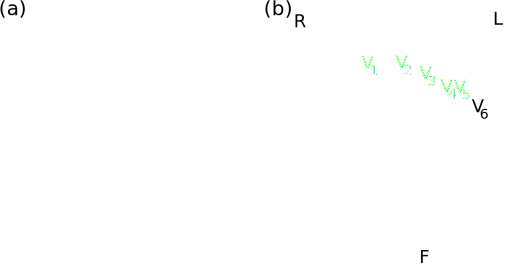
\includegraphics{figures/bsp/thorax_layout}
\caption[Torso showing embedded atrium and lead locations]{
\label{fig:bsp:torso}
(a) Torso geometry used in this study.
The torso geometry, shown unrefined for clarity is shown as a wireframe.
The lungs are shown in blue, the blood masses in red.
The atrium is visible above the bloodmasses.
(b) Solid torso geometry showing the locations used for the simulated
electrodes.
}
\end{figure}

The atrial model constructed in the previous chapter was positioned within the
torso using the descriptions of Ho and S\'{a}nchez-Quintana~\cite{Ho2009}
with the ventricular meshes from the original torso used as an additional guide.
First, the model was centred in the atrial co-ordinate system.
Using the z-x-z convention for Euler angles~\cite{Goldstein1980} acting on the heart
(rather than the co-ordinate system of the heart), the atrium was rotated by
$\left(315, 135, 310\right)$.
Following rotation, a translation of $\left(-0.003, -0.075, -0.217\right)$ was
applied to the atrium.
Several of the triangular elements were picked as the sites of the ECG
electrodes.
The electrode locations are shown in figure~\ref{fig:bsp:torso},(b).
Conductances used for the various compartments of the torso are shown in
table~\ref{tbl:bsp:conductances}.
\begin{table}[h]
    \caption[Conductances of torso compartments]{
        Conductances used for the various compartments of the torso for solving
        the boundary element method~\cite{Seger2004}.
    }
    \begin{tabular}{l r}
     \toprule
     Tissue & Conductivity \\
     \midrule
     Torso & $0.2\,\text{Sm}^{\text{-1}}$ \\
     Lungs & $0.08\,\text{Sm}^{\text{-1}}$ \\
     Blood & $0.6\,\text{Sm}^{\text{-1}}$ \\
     \bottomrule
     \label{tbl:bsp:conductances}
    \end{tabular}
\end{table}

\section{Computational Implementation}

The program which solved the equations and generated the potentials at each of
the elements of the geometry was written in the Fortran 95 programming language.
The $\mathbf{A}$ matrix from (\ref{eqn:bsp:matrix}) was constructed using the
method proposed by van Oosterom and Strackee~\cite{Oosterom1983}\ to
estimate the solid angle subtended by each triangular element.
A subroutine written in C was used to read in the gzip or xz compressed
data files corresponding to each snapshot in time (\ms{1}) generated by the
atrial model.
The impressed current density at each node of the tissue was calculated using
(\ref{eqn:bsp:ji}).
To reduce computational time and memory requirements, the atrial geometry was
divided into 10x10x10 node blocks, around 4000 of which actually had active
nodes within.
The dipoles generated by each active node were aggregated and considered to act
at the centroid of the block determined from the distribution of active nodes
within the block.
These `large' dipoles were then used as the source terms in
(\ref{eqn:bsp:infinite}).
To reduce computation time, the equations were formed into 3 sets of coefficient
matrices, corresponding to the x, y and z components of the radius vector.
These were then multiplied by the relevant dipole components and the results
summed to calculate the potential in the centre of each element.
Decreasing the block size to 5x5x5 nodes had a negligible effect on the computed
body surface potential.
From these dipoles, the $\mathbf{B}$ matrix was calculated.

To solve the resulting set of equations, the LAPACK~\cite{lapack} library was
used.
The $\mathbf{A}$ matrix was factorized using the SGETRF sub-routine.
Numerical experiments determined that only single precision arithmetic was
required.
Solutions calculated using double and single precision showed differences only at
the limits of single precision accuracy--approximately 7 significant figures.
Since the torso is static this need only be done once, at the start of the
calculations.
The SGETRS sub-routine was then used to solve (\ref{eqn:bsp:saluphijone}) and
(\ref{eqn:bsp:saluphijstar}) for each time snapshot using this factorised
matrix.
The zero potential, required for the consistency criterion of Salu, was chosen
to be at element 1 of the mesh.
This element is located at the top of the mesh, at the `neck'.
Generating the body surface potential took one core of horace approximately 60
minutes for \unit{2}{s}\ of atrial activity using the original mesh.
Using the fully refined mesh required approximately 190 minutes for the same
computation.

After computation of the potentials at all points on the body surface, the
results were post-processed to extract the ECG.
These data were stored in a JSON~\cite{json}\ formatted file which contained
arrays representing the voltage of each of the 12 leads, the time step between
each point and, optionally, information on the parameters used by the BSP
algorithm.
JSON offers a lightweight alternative to XML, whilst still being highly readable
without the aid of computer translation.
The high-precision ECG signals, typically at a frequency of \unit{1}{kHz}\
were been passed through a digital low-pass filter at \unit{100}{Hz},
corresponding to the typical frequency response of a clinical ECG unit, from
\unit{0.5}{Hz}\ to \unit{100}{Hz}.
Using the three limb leads (LA, LL, RA) the WCT was computed and used to
construct isopotential maps.
Whilst the algorithm employed offers a natural zero potential, the use of the
WCT allows for direct comparison with clinical studies which almost exclusively
employ the WCT for this purpose~\cite{Taccardi1966,Mirvis1980}


\section{Simulating Sinus Rhythm}

To simulate the P-wave body surface potential and ECG for the atrium in sinus
rhythm, the atrial model developed in the previous chapter was used.
The simulation of the electrical activity involved the full fibre orientation
description with an anisotropy ratio of 1:9.
There was heterogeneous cell electrophysiology used, with differential
electrophysiology for the atrial myocyte, pectinate muscle and crista
terminalis cells.
The atrium was paced at the site corresponding to the sinus node at a frequency
of \unit{1}{Hz}\ for \unit{2}{s}.
The body surface potential was calculated both with and without the presence of
internal inhomogeneities by setting the internal conductivity of the relevant
compartment to the value in table~\ref{tbl:bsp:conductances}\ to include that
compartment, or to the torso conductivity to remove its influence.

\subsection{Simulated Body Surface Potential Maps}

The Body Surface Potential Maps (BSPM) were constructed from the output of the
simulations.
In the following descriptions, the distribution is described using the using the
coordinate system of the body rather than of the image.
Note that the raw signals are presented here, that is to say there is no
filtering performed on the signals in the time domain.

\begin{figure}
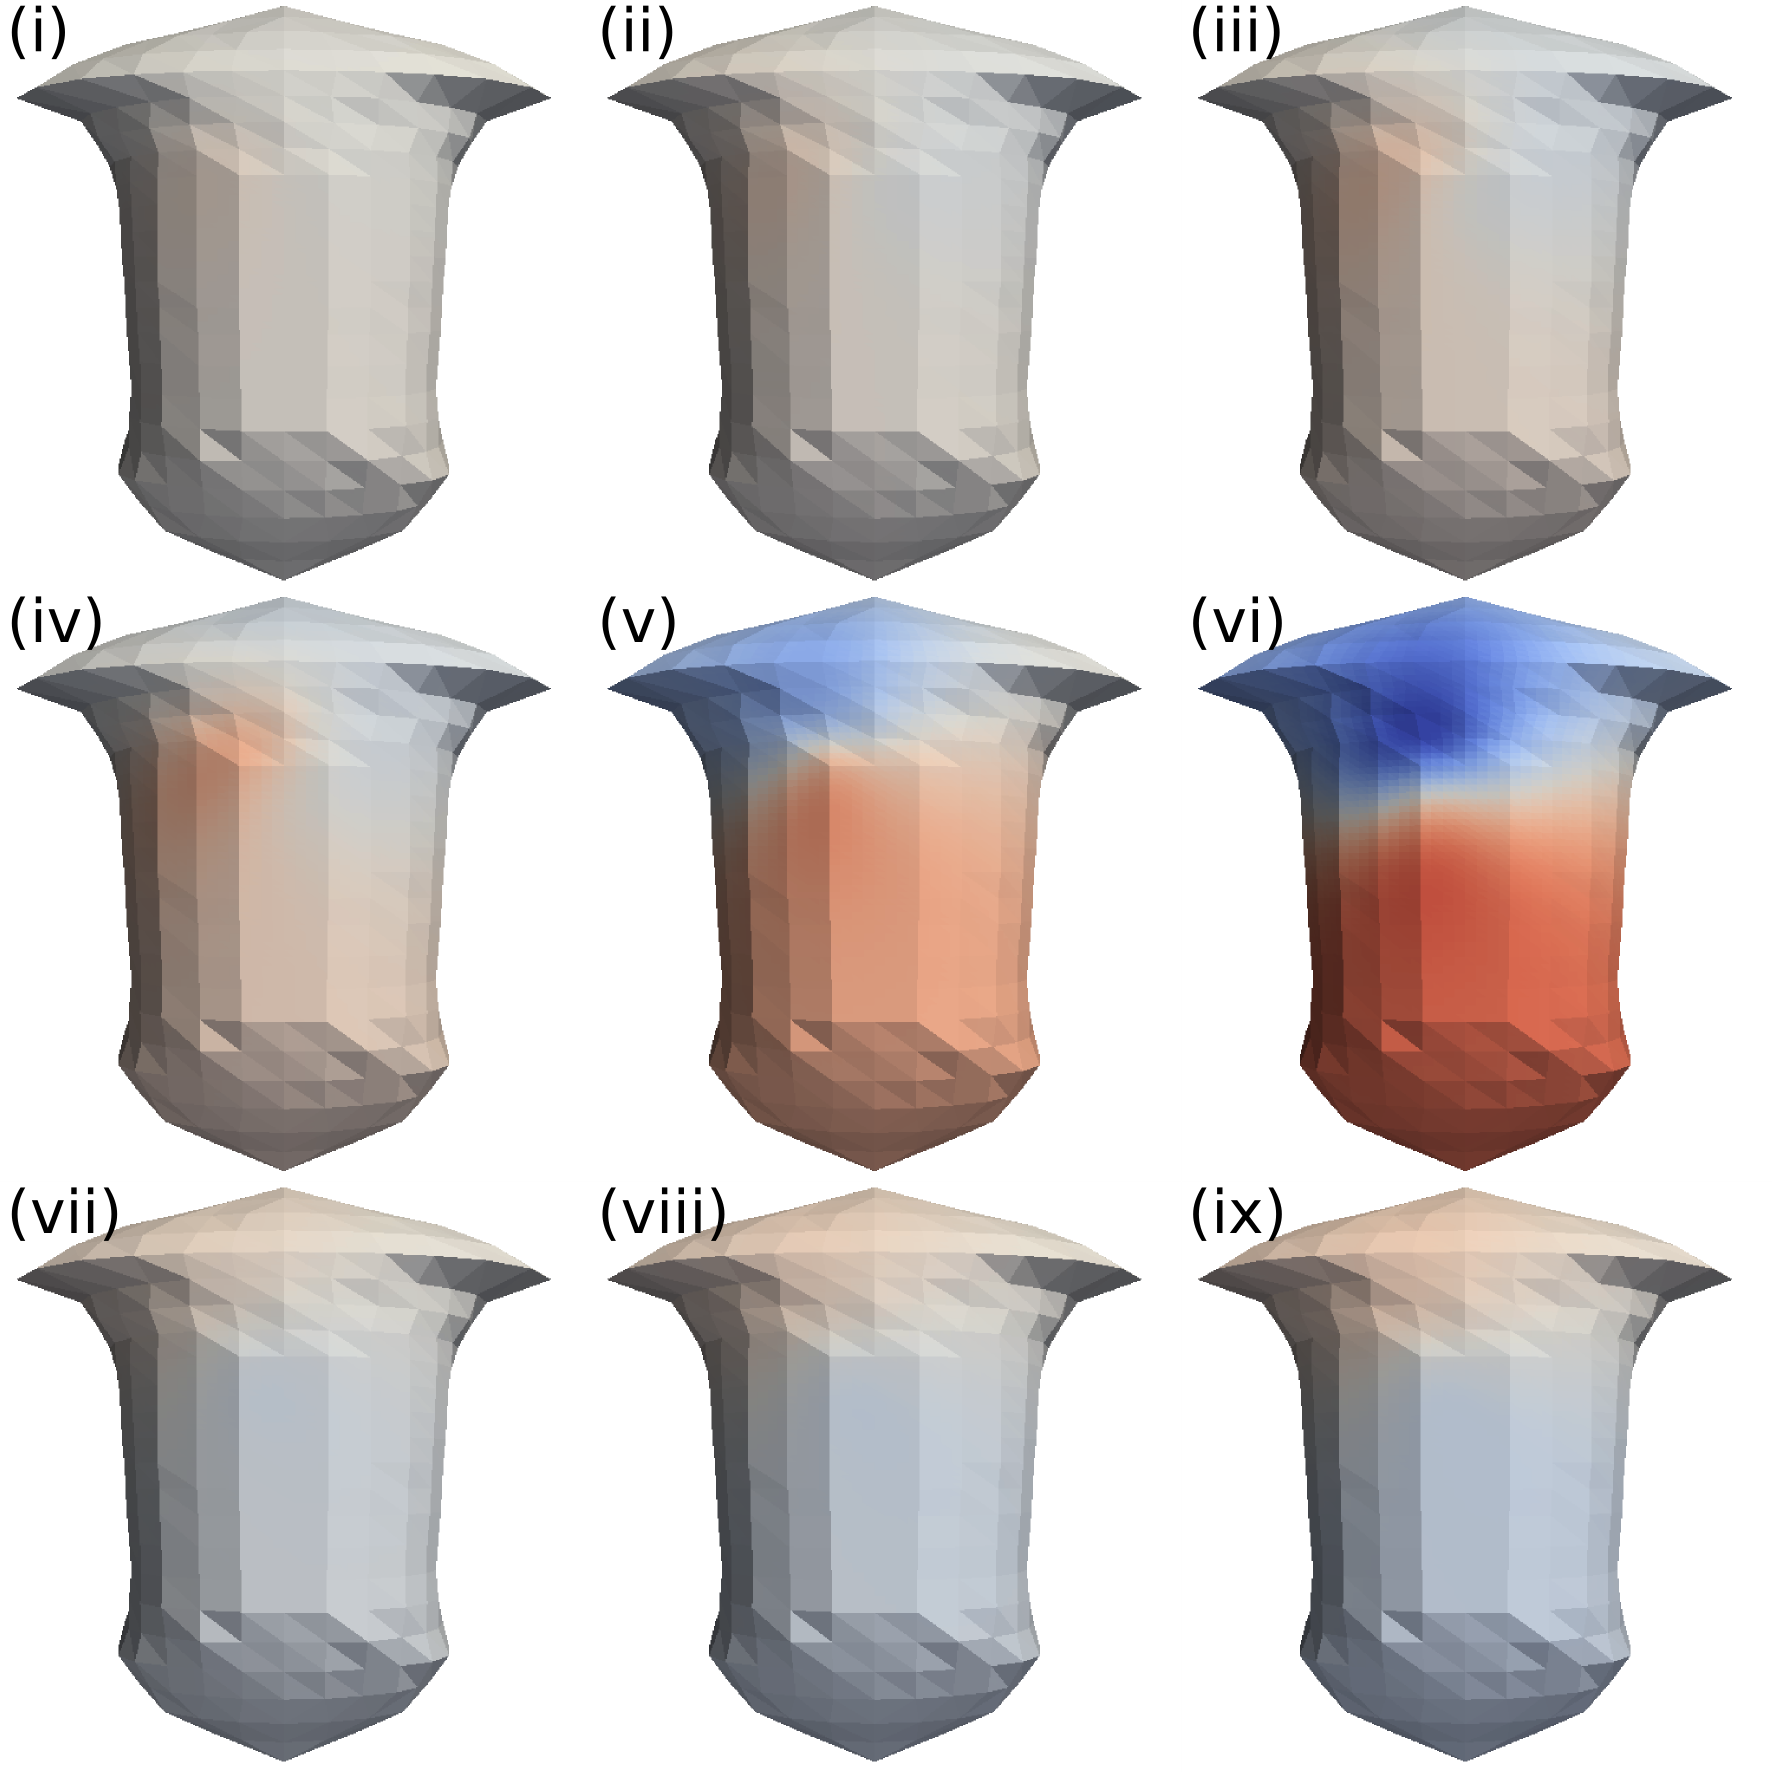
\includegraphics{figures/bsp/bsp_torso}
\caption[Body Surface Potential snapshots, homogeneous torso]{
\label{bsp:fig:homo_bsp}
Simulated BPSM during sinus rhythm with a homogeneous
torso.
Blue represents negative potentials, and red positive ones, relative to the zero
defined by the Wilson's central terminal.
The torso begins approximately isopotential before a distinct pattern of
potential, with an area of negative potential over the upper right lung and an
area of positive potential on the lower torso.
This pattern then reverses during repolarization, although the magnitudes are
much lower.
The maximum potential observed is \mv{0.334}\ and the minimum is \mv{-0.412}.
Snapshots shown for \ms{10}\ (i), \ms{15}\ (ii), \ms{20}\ (iii), \ms{25}\ (iv),
\ms{40}\ (v), \ms{60}\ (vi), \ms{180}\ (vii), \ms{200}\ (viii) and \ms{220}\
(ix)
}
\end{figure}

The evolution of the body surface potential on a homogeneous torso is shown in
figure~\ref{bsp:fig:homo_bsp}.
The timings of the body surface potential snapshots correspond to the snapshots
of membrane potential shown in figure~\ref{fig:atrium:validation:main}.
The potential distribution starts off very close to uniform in frame (i) at
\ms{10}\ after initial excitation.
Only excitation and repolarization wavefronts generate dipoles and in the
initial milliseconds the excitation wavefront is very small.
In \ref{bsp:fig:homo_bsp}(iv) (\ms{25} after initial stimulus) there is an area
of positive potential beginning to appear over the lower right lung, caused by
the spread of excitation over the pectinate muscles.
By frames (v) and (vi), the regions of different potential are much more
regularly distributed with a predominately negative region centred on the upper
right lung and a positive region over the lower torso, centered further to the
right than the left.
The excitation wavefront is moving towards the legs.

The three frames (vii--ix) corresponding the to the plateau and beginnings of the
repolarization show a much more diffuse arrangement of potentials.
The distribution is approximately the mirror image of that seen during
depolarisation, with the predominantly positive regions over the right shoulder.
The diffuse pattern of potentials is caused by the slower repolarization of
atrial myocytes compared to their depolarisation.
It does not show a disturbance from the smooth pattern as seen for
depolarisation in frame (iv) as the repolarization is less influenced by the
underlying fibre structure.


\begin{figure}
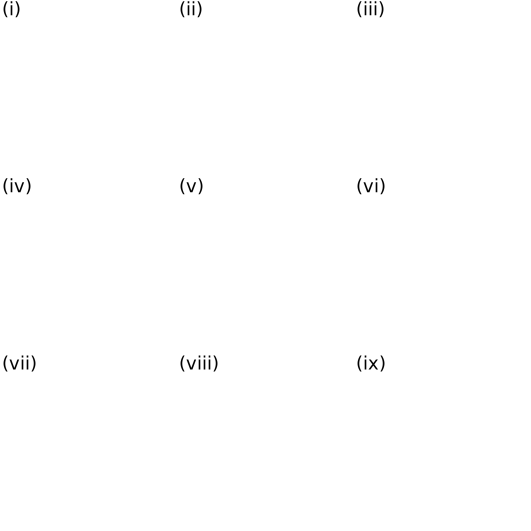
\includegraphics{figures/bsp/bsp_lungs}
\caption[Body Surface Potential snapshots, with lungs]{
\label{bsp:fig:lungs_bsp}
Simulated body surface potential plots during sinus rhythm with lungs assigned
conductivity from table~\ref{tbl:bsp:conductances}.
Blue represents negative potentials, and red positive ones, relative to the zero
defined by the Wilson's central terminal.
The torso begins approximately isopotential before a distinct pattern of
potential, with an area of negative potential over the upper right lung and
area of positive potential on lower half of the torso.
The positive peak is higher than that observed without lungs and the negative
region appears to be larger.
The positive--negative pattern then reverses during repolarization, with the
upper torso having a positive potential.
The maximum potential observed is \mv{0.379}\ and the minimum is \mv{-0.475}.
Snapshots shown for \ms{10}\ (i), \ms{15}\ (ii), \ms{20}\ (iii), \ms{25}\ (iv),
\ms{40}\ (v), \ms{60}\ (vi), \ms{180}\ (vii), \ms{200}\ (viii) and \ms{220}\
(ix)
}
\end{figure}

The evolution of the body surface potential with lungs is shown in
figure~\ref{bsp:fig:lungs_bsp}.
In \ref{bsp:fig:lungs_bsp}(iv) (\ms{25} after initial stimulus) a peak is
beginning to appear over the lower right lung, caused as excitation starts to
spread through the crista terminalis and pectinate muscles.
By frames (v) and (vi), the potential is much more regularly distributed.
In contrast to the simulation without lungs, the region of predominantly
negative potential seems to be larger in spatial extent than that which is
observed without lungs.
The corresponding positive peak does not seem to be any more extended, but it
does have a greater magnitude.
It appears that the lungs act to give a slight amplification
effect, increasing the ranges of potential seen~\cite{Gulrajani1983}.

The three frames (vii--ix) corresponding the to the plateau and beginnings of the
repolarization show a much more diffuse arrangement of potentials.
The distribution is approximately the mirror image of that seen during
depolarisation, with the predominantly positive regions over the right shoulder.
The effects of the lungs are almost unnoticeable when compared to the
simulations in the homogeneous torso.

\begin{figure}
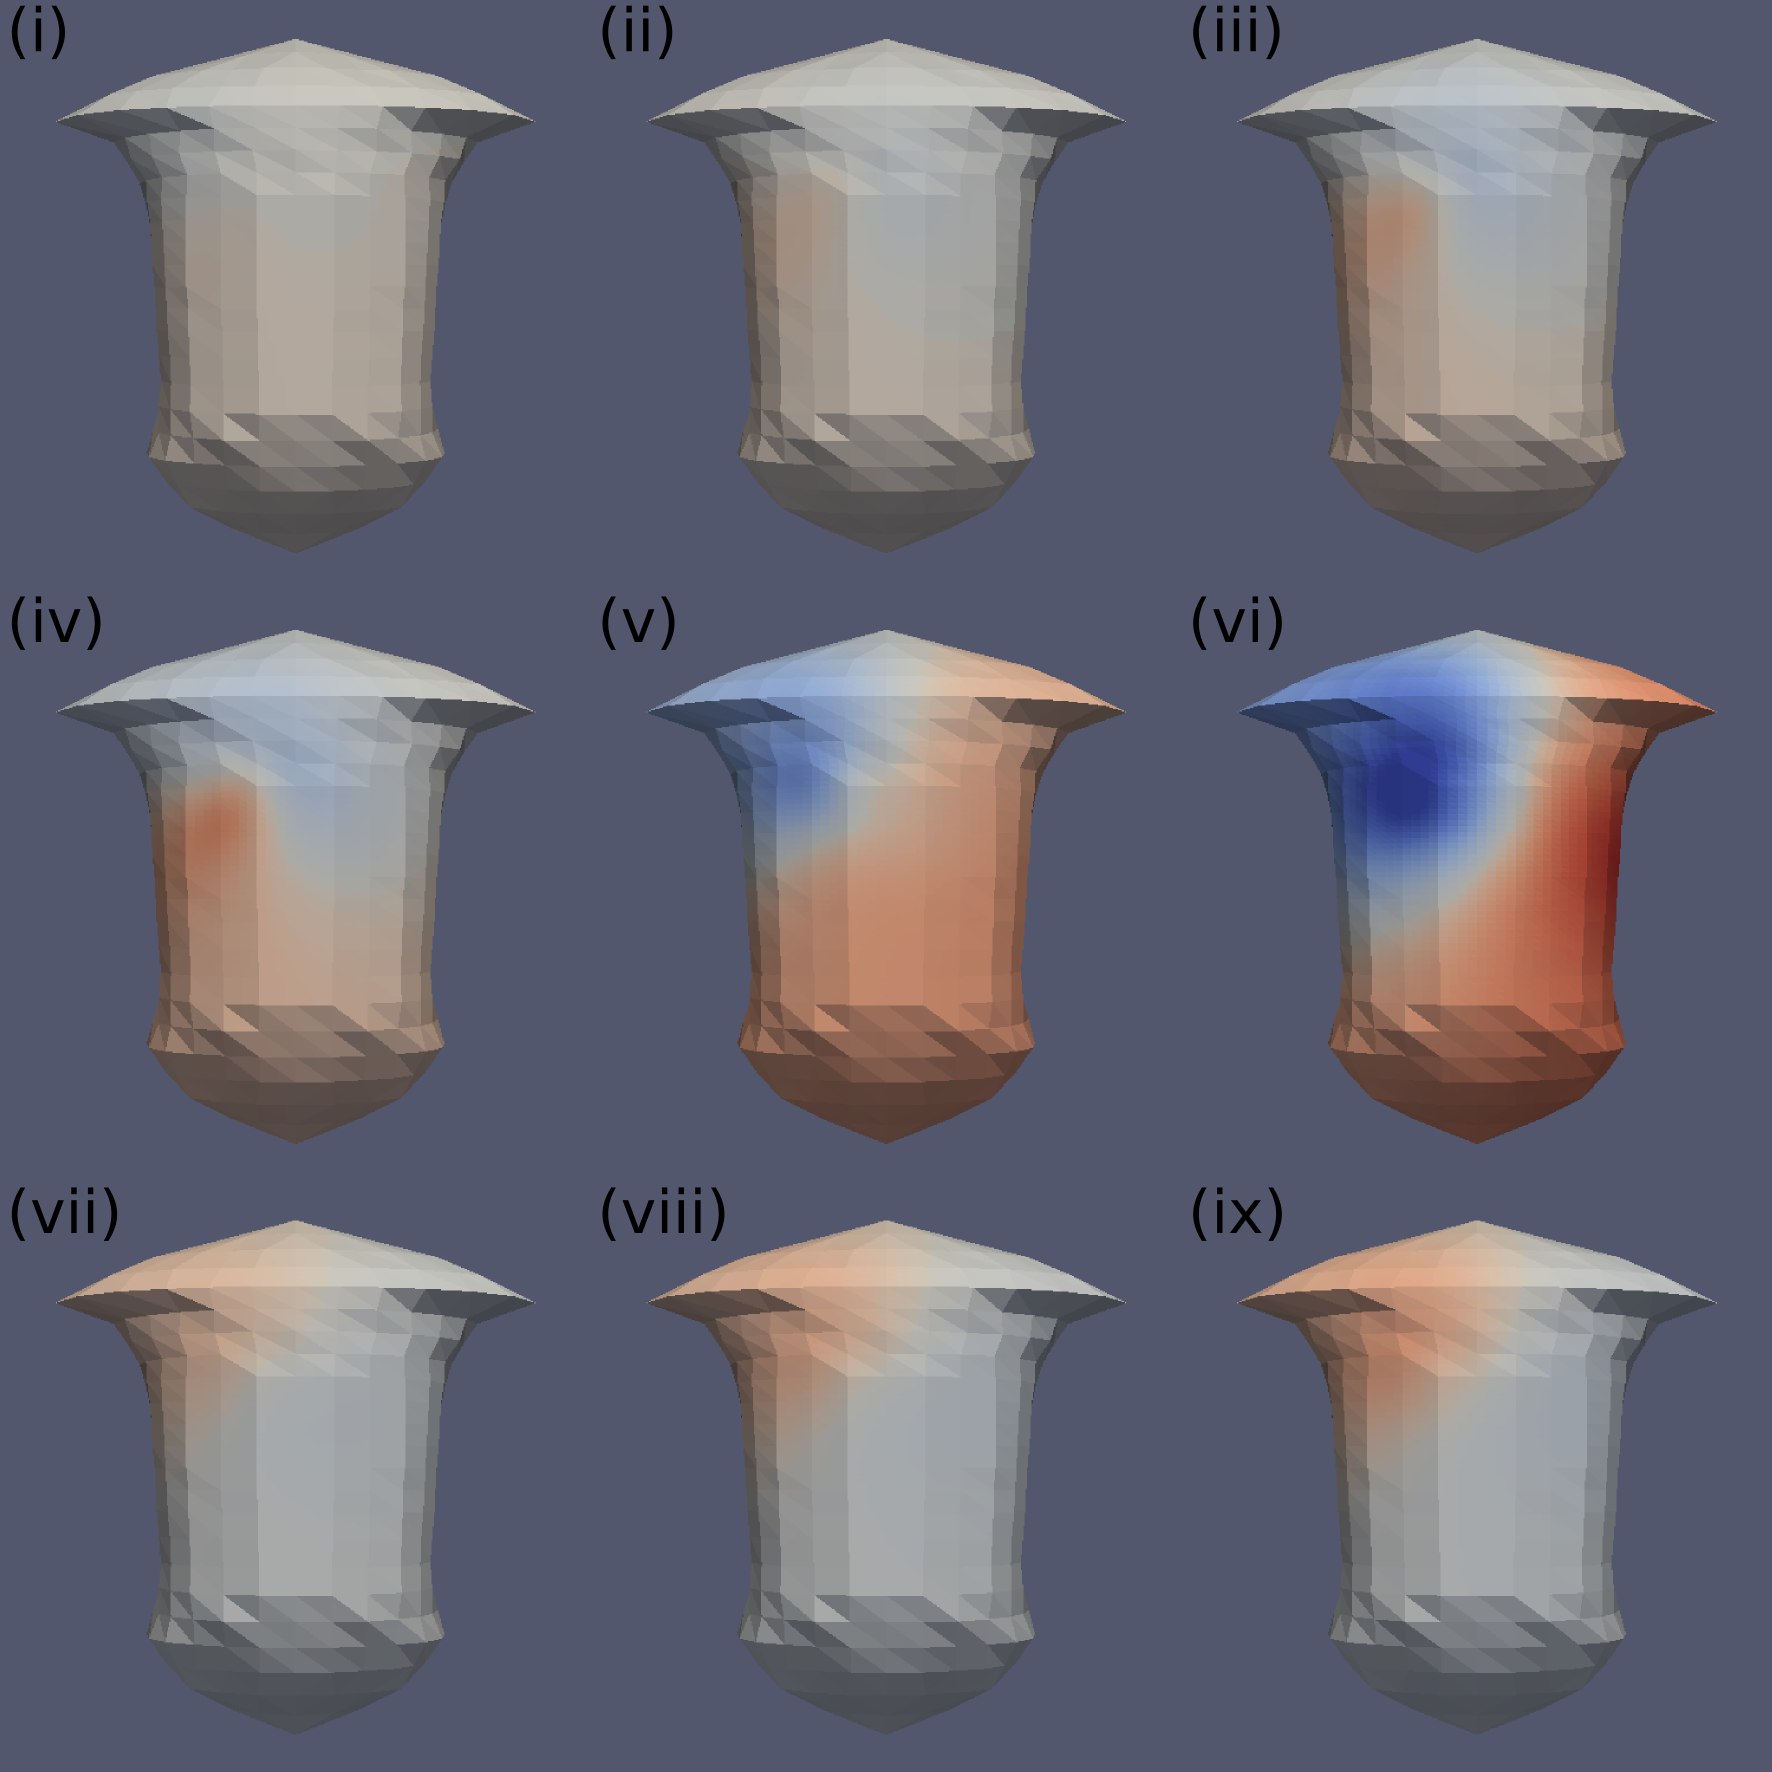
\includegraphics{figures/bsp/bsp_blood}
\caption[Body Surface Potential snapshots, with blood masses]{
\label{bsp:fig:blood_bsp}
Simulated body surface potential plots during sinus rhythm with blood masses assigned
conductivity from table~\ref{tbl:bsp:conductances}.
Blue represents negative potentials, and red positive ones, relative to the zero
defined by the wilson's central terminal.
The torso begins approximately isopotential before a distinct pattern of
potential, with an area of negative potential over the right shoulder and an
area of positive potential below.
The pattern of potentials is similar to that observed in the simulation with a
homogeneous torso, but it has a smaller magnitude.
This pattern then reverses during repolarization.
The maximum potential observed is \mv{0.304}\ and the minimum is \mv{-0.406}.
Snapshots shown for \ms{10}\ (i), \ms{15}\ (ii), \ms{20}\ (iii), \ms{25}\ (iv),
\ms{40}\ (v), \ms{60}\ (vi), \ms{180}\ (vii), \ms{200}\ (viii) and \ms{220}\
(ix)
}
\end{figure}

The evolution of the body surface potential with blood masses present is shown in
figure~\ref{bsp:fig:blood_bsp}.
The potential distribution is initially almost uniform, when  in frame (i) at
\ms{10}\ after initial excitation.
In \ref{bsp:fig:blood_bsp}(iv) a positive potential is beginning to appear over
the lower right lung, caused by the rapid conduction along the crista
terminalis and associated structures.
In contrast to the simulations with the lungs present, or in the homogeneous
torso, this appears to have a relatively well defined peak compared with the
more diffuse potential seen in those simulations.
The corresponding negative potential area is more widely spread than in those
cases, extending further down the torso.
By frames (v) and (vi), the pattern of potential observed on the body surface is
very close to that seen in the homogeneous torso, although the maxima and minima
are less extreme in the frames where the blood masses are included.
The blood masses also seem to act as a focus, with the peak visible in frame (v)
much smaller in spatial extent than the peak which is observed in the
corresponding frames both in the homogeneous torso and in the torso with lungs.
This effect is much less noticeable by frame (vi) however.

The three frames (vii--ix) corresponding the to the plateau and beginnings of the
repolarization show a much more diffuse arrangement of potentials.
The arrangement looks very similar to the corresponding frames from the
homogeneous calculations.


\begin{figure}
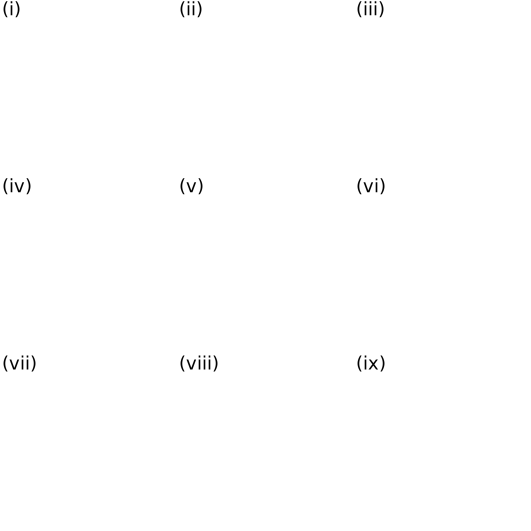
\includegraphics{figures/bsp/bsp_all}
\caption[Body Surface Potential snapshots, with all inhomogeneities]{
\label{bsp:fig:all_bsp}
Simulated body surface potential plots during sinus rhythm with all
inhomogeneities assigned conductivities from table~\ref{tbl:bsp:conductances}.
Blue represents negative potentials, and red positive ones, relative to the zero
defined by the Wilson's central terminal.
The torso begins approximately isopotential before a distinct pattern of
potential, with an area of negative potential over the upper right lung and an
area of positive potential below it.
This pattern then reverses during repolarization.
The maximum potential observed is \mv{0.359}\ and the minimum is \mv{-0.465}.
Snapshots shown for \ms{10}\ (i), \ms{15}\ (ii), \ms{20}\ (iii), \ms{25}\ (iv),
\ms{40}\ (v), \ms{60}\ (vi), \ms{180}\ (vii), \ms{200}\ (viii) and \ms{220}\
(ix)
}
\end{figure}

The evolution of the body surface potential with all inhomogeneities present is
shown in figure~\ref{bsp:fig:all_bsp}.
In (iv) an isolated peak is beginning to appear over the lower
right lung.
This is closer to the potential distribution shown in the simulations with just
blood masses included than those where lungs are present or where there a
homogeneous torso.
In contrast to this, frames (v) and (vi) show a distribution of potential much
closer to that seen in the simulations where lungs are present, with a larger
area of negative potential than is observed in the homogeneous torso.
The final stages of evolution of the P-wave body surface potential, shown in
frames (vii--ix) show a diffuse pattern, similar to that seen in all the other
simulations.

\subsection{Simulated Electrocardiograms}

In this section, electrocardiograms derived from the BSP distribution are
presented for sinus rhythm.
All of the leads show a minor artifact during the first
$2\text{--}4\,\text{ms}$, due to the stimulation protocol employed.
Disregarding this, the following classifications are used~\cite{Kistler2006}.
A positive, or upright, P-wave is one that attains a potential of
$\geq$\mv{0.05}\ and remains above the 0 potential baseline for duration of the
P-wave.
A negative, or inverted, P-wave is one that attains a potential of
$\leq$\mv{-0.05}\ and remains below the baseline for the duration of the P-wave.
A biphasic P-wave is one that is both positive and negative, following the
previous two definitions.


\begin{figure}
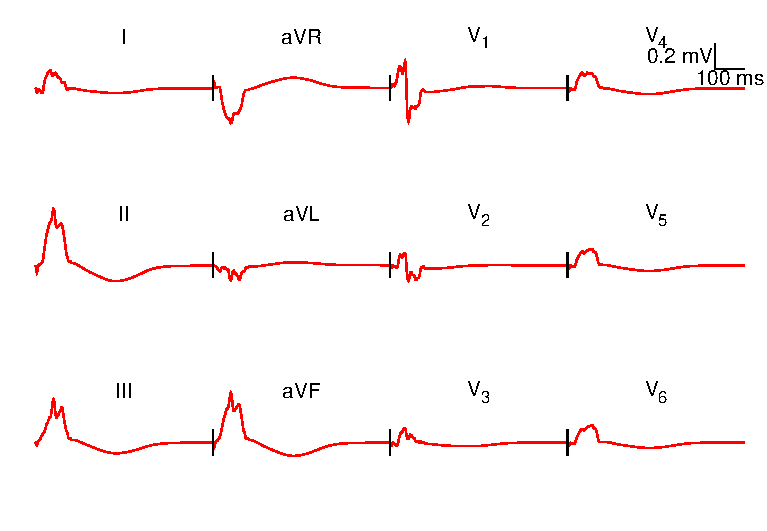
\includegraphics{figures/bsp/ecg_torso}
\caption[12 lead P-wave ECG during sinus rhythm with homogeneous torso]{
\label{bsp:fig:ecg_torso}
Simulated P-Wave ECG traces during sinus rhythm with homogeneous torso.
One complete action potential cycle is shown.
The stimulus is initiated at $t = 0$ in all traces.
All traces have been smoothed with a \unit{100}{Hz}\ low-pass filter, to
simulate the typical frequency response of clinical ECG units.
}
\end{figure}

The ECG derived from the body surface potential simulations with a homogeneous
torso is shown in figure~\ref{bsp:fig:ecg_torso}.
The P-wave has a duration of \ms{109}\ in lead II and an amplitude of \mv{0.466}.
The maximum and minimum potential differences observed in the leads are
\mv{+0.446}\ and \mv{-0.275}\ seen in lead II and lead aVR, respectively.
The P-wave is positive in leads I, II, III, aVF and $\text{V}_{\text{3--6}}$.
It is positive--negative biphasic in $\text{V}_{\text{1}}$ and $\text{V}_{\text{2}}$.
It is inverted in leads aVR and aVL.

The atrial repolarization wave, the $\text{T}_{\text{P}}$ wave, is easily
visible in most leads.
It is very flat, almost to the point of invisibility, in leads I, aVL and
$\text{V}_{\text{1--3}}$.
In all the leads in which it appears, it is inverted compared to the P-wave in
that lead and has a lower (less than 50\% in all leads) amplitude.
It appears to start immediately after the P-wave in all leads.
The $\text{T}_{\text{P}}$ is broader than the P-wave, corresponding to the lower
speed of repolarization.

\begin{figure}
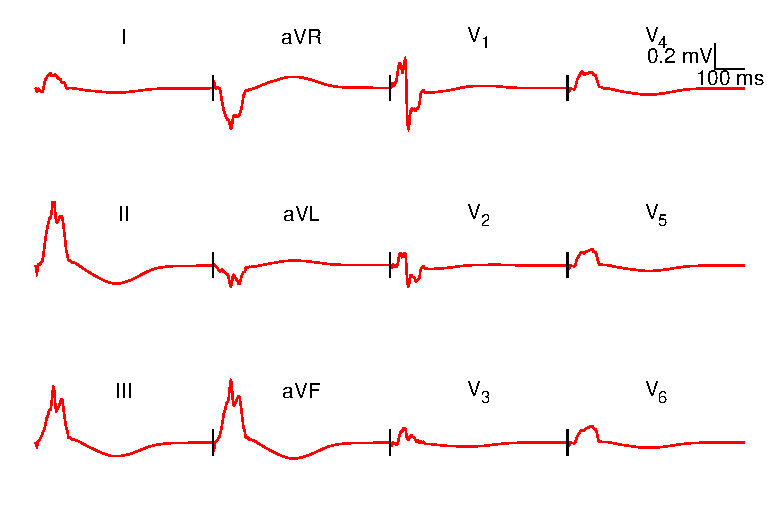
\includegraphics{figures/bsp/ecg_lungs}
\caption[12 lead ECG during sinus rhythm, lungs present.]{
\label{bsp:fig:ecg_lungs}
Simulated P-Wave ECG traces during sinus rhythm with inhomogeneous torso.
Lungs assigned conductivity from table~\ref{tbl:bsp:conductances}.
One complete action potential cycle is shown.
The stimulus is initiated at $t = 0$ in all traces.
All traces have been smoothed with a \unit{100}{Hz}\ low-pass filter.
This is to closer emulate the frequency response of a typical clinical ECG unit.
}
\end{figure}

The ECG corresponding to the simulations with inhomogeneous lungs is shown in
figure~\ref{bsp:fig:ecg_lungs}.
The P-wave has a duration of \ms{117}\ in lead II and an amplitude of \mv{+0.535}.
The maximum and minimum potential differences observed in the leads are
\mv{+0.535}\ and \mv{-0.319}\ seen in lead II and lead $\text{V}_{\text{1}}$, respectively.
The P-wave is positive in leads I, II, III, aVF and $\text{V}_{\text{3--6}}$.
It is positive--negative biphasic in $\text{V}_{\text{1}}$ and $\text{V}_{\text{2}}$.
It is inverted in leads aVR and aVL.
In general, the presence of the lungs appears to amplify the signal compared to
the simulations without lungs.

The $\text{T}_{\text{P}}$ wave is
visible in most leads, though in the leads which did not attain very high
potentials (I, aVL, $\text{V}_{\text{1--3}}$) it is very flat.
In all the leads in which it appears, it is inverted compared to the P-wave in
that lead and has a lower (less than 50\% in all leads) amplitude.
It appears to start immediately after the P-wave in all leads.
The $\text{T}_{\text{P}}$ is broader than the P-wave in all leads.


\begin{figure}
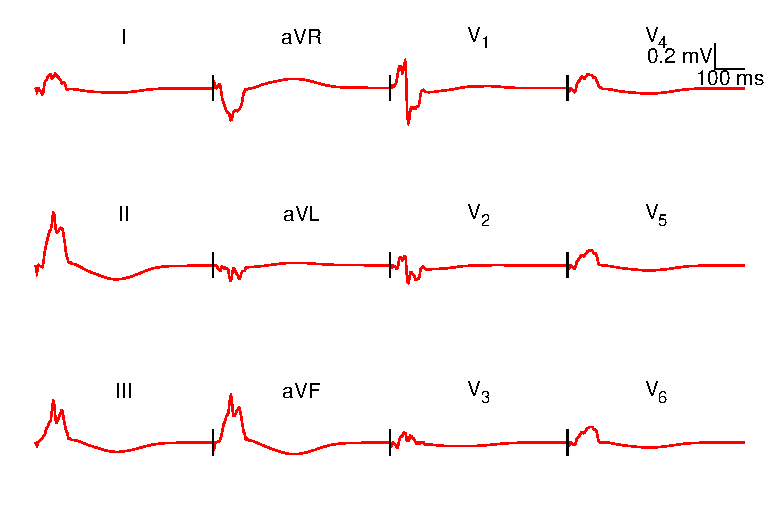
\includegraphics{figures/bsp/ecg_blood}
\caption[12 lead ECG during sinus rhythm, bloodmasses present.]{
\label{bsp:fig:ecg_blood}
Simulated P-Wave ECG traces during sinus rhythm with inhomogeneous torso.
Blood masses assigned conductivity from table~\ref{tbl:bsp:conductances}.
One complete action potential cycle is shown.
The stimulus is initiated at $t = 0$ in all traces.
All traces have been smoothed with a \unit{100}{Hz}\ low-pass filter.
This is to closer emulate the frequency response of a typical clinical ECG unit.
}
\end{figure}

The ECG corresponding to the simulations with inhomogeneous blood masses is shown in
figure~\ref{bsp:fig:ecg_blood}.
The P-wave has a duration of \ms{100}\ in lead II and an amplitude of \mv{+0.415}.
The maximum and minimum potential differences observed in the leads are
\mv{+0.415}\ and \mv{-0.275}\ seen in lead II and lead $\text{V}_{\text{1}}$, respectively.
The P-wave is positive in leads I, II, III, aVF and $\text{V}_{\text{3--6}}$.
It is positive--negative biphasic in $\text{V}_{\text{1}}$ and $\text{V}_{\text{2}}$.
It is inverted in leads aVR and aVL.
The presence of the bloodmasses generally acts to reduce the amplitudes of the
P-wave ECG.

The $\text{T}_{\text{P}}$ wave is
visible in most leads, though in the leads which did not attain very high
potentials (I, aVL, $\text{V}_{\text{1--3}}$) it is very flat.
In all the leads in which it appears, it is inverted compared to the P-wave in
that lead and has a lower (less than 50\% in all leads) amplitude.
It appears to start immediately after the P-wave in all leads.
The $\text{T}_{\text{P}}$ is broader than the P-wave in all leads.

\begin{figure}
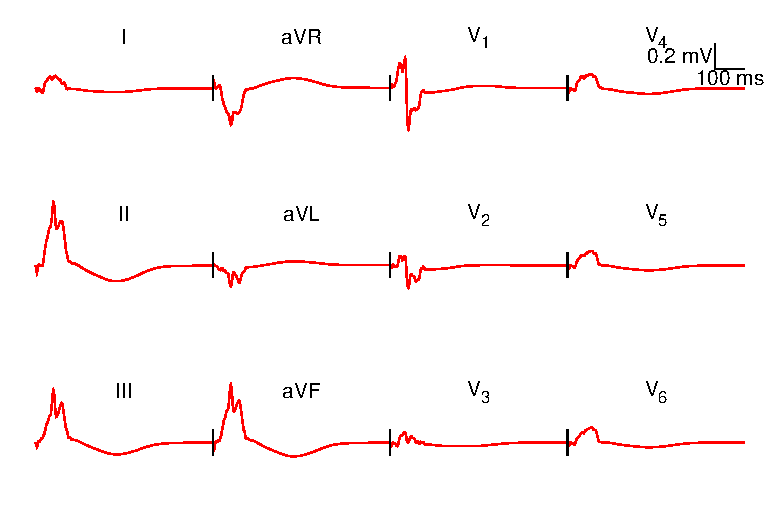
\includegraphics{figures/bsp/ecg_all}
\caption[12 lead ECG during sinus rhythm, all internal inhomogeneities present.]{
\label{bsp:fig:ecg_all}
Simulated P-Wave ECG traces during sinus rhythm with inhomogeneous torso.
Lungs and blood masses assigned conductivity from table~\ref{tbl:bsp:conductances}.
One complete action potential cycle is shown.
The stimulus is initiated at $t = 0$ in all traces.
All traces have been smoothed with a \unit{100}{Hz}\ low-pass filter, a typical
upper limit of frequency response in clinical ECG machines.
}
\end{figure}

The ECG corresponding to the simulations with all inhomogeneities considered is shown in
figure~\ref{bsp:fig:ecg_all}.
The P-wave has a duration of \ms{103}\ in lead II and an amplitude of \mv{+0.497}.
The maximum and minimum potential differences observed in the leads are
\mv{+0.497}\ and \mv{-0.325}\ seen in lead II and lead $\text{V}_{\text{1}}$, respectively.
The P-wave is positive in leads I, II, III, aVF and $\text{V}_{\text{3--6}}$.
It is positive--negative biphasic in $\text{V}_{\text{1}}$ and $\text{V}_{\text{2}}$.
It is inverted in leads aVR and aVL.
When the blood masses and the lungs are both present, the resulting ECG is a
mixture of the effects of both sets of inhomogeneities.
This results in an ECG which generally has lesser amplitudes than those observed
in the simulations where only the lungs are present, though greater than the
magnitudes where there is just the torso.

The $\text{T}_{\text{P}}$ wave is visible in
most leads, though in the leads which did not attain very high potentials (I,
aVL, $\text{V}_{\text{1--3}}$) it is very flat.
In all the leads in which it appears, it is inverted compared to the P-wave in
that lead and has a lower (less than 50\% in all leads) amplitude.
It appears to start immediately after the P-wave in all leads.
The $\text{T}_{\text{P}}$ is broader than the P-wave in all leads, corresponding
to the lower speed of repolarization.

A summary table of the maxima or minima of the leads is shown in
table~\ref{tbl:bsp:ecg}.


\begin{table}
    \caption[Maximum and minimum potentials observed in ECG leads]{
        Maximum and minimum potentials observed in the twelve leads of the ECG
        for differing inhomogeneities considered.
        Torso corresponds to the homogeneous case, lungs to the case where the
        lungs are given a conductivity from table~\ref{tbl:bsp:conductances},
        blood to case where the blood masses were assigned the conductivity from
        table~\ref{tbl:bsp:conductances} and all, for when both lungs and blood
        masses were assigned differing conductivities.
        For upright and inverted leads, only one potential is given, the maximum
        or minimum potential observed, respectively.
        For biphasic leads, both the maximum and minimum potentials are given.
        All values in mV.
    }
    \begin{tabular}{ l r r r r }
    \toprule
    Lead & Torso & Lungs & Blood & All \\
    \midrule
    I                       & $+0.139$ & $+0.117$ & $+0.113$ & $+0.097$ \\
    II                      & $+0.446$ & $+0.535$ & $+0.415$ & $+0.497$ \\
    III                     & $+0.341$ & $+0.435$ & $+0.328$ & $+0.414$ \\
    aVR                     & $-0.275$ & $-0.317$ & $-0.251$ & $-0.290$ \\
    aVL                     & $-0.118$ & $-0.167$ & $-0.121$ & $-0.165$ \\
    aVF                     & $+0.394$ & $+0.485$ & $+0.372$ & $+0.455$ \\
    $\text{V}_{\text{1}}$   & $+0.208/-0.265$ & $+0.227/-0.319$ & $+0.211/-0.275$ & $+0.233/-0.325$ \\
    $\text{V}_{\text{2}}$   & $+0.095/-0.125$ & $+0.093/-0.166$ & $+0.068/-0.142$ & $+0.075/-0.180$ \\
    $\text{V}_{\text{3}}$   & $+0.109$ & $+0.113$ & $+0.076$ & $+0.080$ \\
    $\text{V}_{\text{4}}$   & $+0.123$ & $+0.129$ & $+0.108$ & $+0.108$ \\
    $\text{V}_{\text{5}}$   & $+0.127$ & $+0.125$ & $+0.116$ & $+0.113$ \\
    $\text{V}_{\text{6}}$   & $+0.133$ & $+0.128$ & $+0.122$ & $+0.116$ \\
    \bottomrule
    \label{tbl:bsp:ecg}
    \end{tabular}
\end{table}

The phase of the signal, that is whether it is rising or falling, does not seem
to be influenced by the presence or absence of
inhomogeneities~\cite{Ramanathan2001a,Gulrajani1983}, only the amplitude.
However, the influence of the inhomogeneities in each lead is not equal, with
some leads being increased and others decreased.
This suggests that the inhomogeneities might have greater importance in the
atria, possibly due to the lower mass of atrial tissue and its thinner walls.

\subsection{Comparisons with Clinical Studies and Information}

Opinions vary on what is considered a `normal'
P-Wave ECG~\cite{Lipman1994,Conover1996,Hampton1997}.
All sources agree that the P-wave should be positive in leads I, II, aVF and
$\text{V}_{\text{4--6}}$ and negative in aVR which the model shows.
Lead III is considered normal if it is positive or biphasic.
None of the three sources agree on the orientation of a normal P-wave in aVL,
but a negative P-wave is considered acceptable.
Leads $\text{V}_{\text{1--3}}$ are considered normal if they are positive in
some of the sources, but others suggest they should, or can be biphasic.
The generated ECGs therefore seem to lie within the normal limits for their
basic phase relationships.

Another notable feature is the presence of the $\text{T}_{\text{P}}$ in many of
the leads, which is not normally observed in clinical ECG recordings.
Its presence in the traces generated by this model is due to a combination of
factors.
The first and most obvious reason is that the traces produced by the model are a
lot `cleaner' than those recorded clinically since there are no problems due to
RF interference from wiring, or skeletal muscle activation.
They are also scaled appropriately to view the P-wave, which has an
amplitude which is approximately an order of magnitude smaller than the
QRS-complex which most 12 lead systems are scaled to view.
There is also the lack of the QRS complex, which often obscures the
$\text{T}_{\text{P}}$ wave.

Macfarlane and Lawrie~\cite{MacFarlane1989b}\ give the P-wave duration in
lead II for males and females in various age groups.
Due to the hybrid nature of the model, it is hard to know which group gives the
most accurate comparison.
The P-wave duration for the fully inhomogeneous model of \ms{103}\ gives good
agreement with both the $104\,\pm\,12.9\,\text{ms}$ reported for a females of
ages 40--49, which is the age of the heart and with the
$103\,\pm\,14.2\,\text{ms}$ figure reported for males of age 18--29, the age of
the torso.
They report the maximum P-wave potential in lead II to be approximately
\mv{0.23}.
The maximum potential observed in the fully heterogeneous case is \mv{+0.497}.
In general, the amplitudes in all leads fall outside the maxima observed in the
clinical data.
This is expected~\cite{Ramanathan2001a,Gulrajani1983,Gulrajani1989,Klepfer1997}\ as internal
inhomogeneities tend to reduce the observed potentials as they `smear' the
electrical signal out over the torso.

Clinical BSPM data for the P-wave has been taken by
Taccardi~\cite{Taccardi1966}\ and Mirvis~\cite{Mirvis1980}.
A comparison of the data taken by Mirvis is shown in
figure~\ref{bsp:fig:mirvis_compare}.
They presented a `typical case' from their study of 40 individuals.
The BSPM generated by the combined atrial and torso model shows quite good
agreement with the experimental BSPM recorded by Mirvis.
The BSPM starts off almost isopotential with a single positive peak.
This then grows in both physical extent and magnitude, moving towards the middle
of the precordial leads.
At \ms{48}\ there are two distinct negative and positive regions, with a single
peak.
This peak then moves off to the left, over the precordial leads.
As the P-wave ends, there is a single negative peak, sitting over leads 1 and 2.
Apart from the obvious, that of amplitude differences, the Mirvis study does
differ slightly from the model.
In general the model's peaks are slightly to the left of those which Mirvis
observed.
In addition, the Mirvis BSPM seems to suggest a P-wave axis which is rotated
slightly, with the zero line sloping upwards from right to left (in the body's
sense), rather than the almost horizontal line observed in the plots from the
model.
However, the essential properties of the Mirvis data are reproduced.
The positive and negative regions are single peaked and a very similar evolution
of potentials is observed.

\begin{figure}
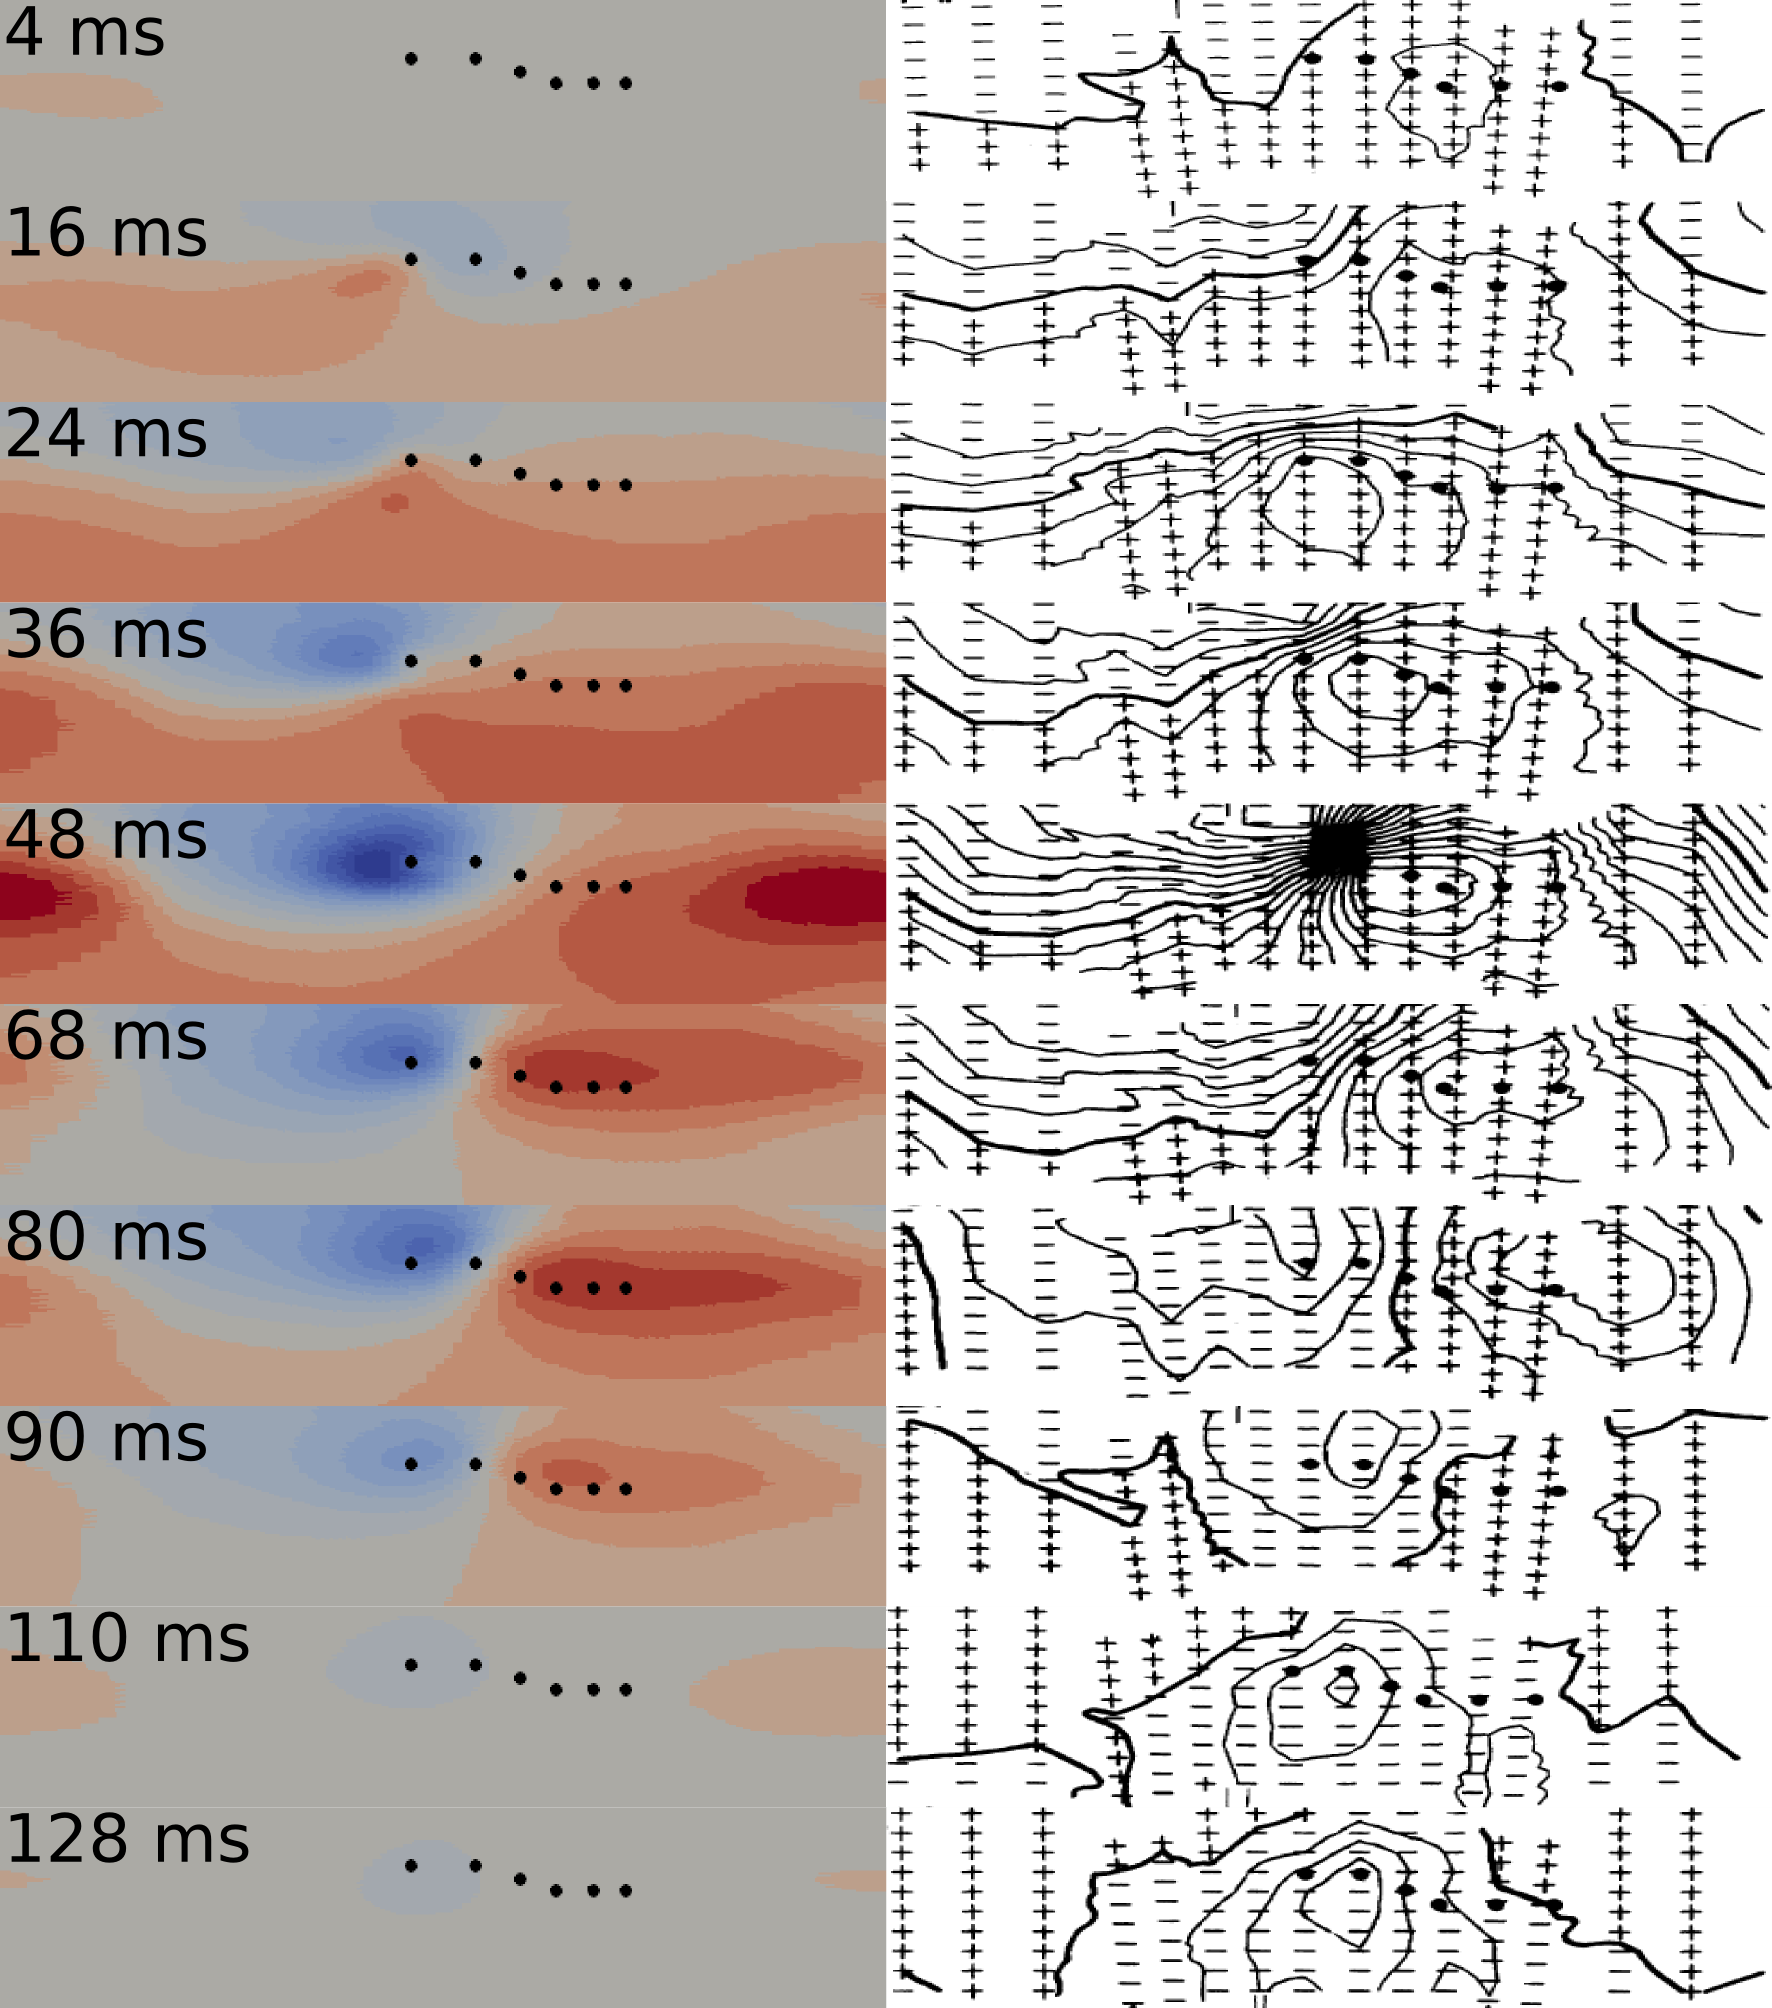
\includegraphics{figures/bsp/mirvis_compare}
\caption[Comparative BSPM from the fully inhomogeneous model and Mirvis]{
\label{bsp:fig:mirvis_compare}
BSPMs generated by the combined torso and heart model (left) compared with
clinical BSPM data recorded by Mirvis~\cite{Mirvis1980} (right).
Precordial leads are shown as black circles (both sides).
On the left, red indicates increasingly positive potentials, blue increasingly
negative and Grey indicates a potential near zero.
On the right, $+$ and $-$ signs indicate regions of positive and negative
potentials, respectively.
Zero potential is the bold contour, other contours in \mv{0.01}\ intervals.
All potentials relative to the Wilson's Central Terminal.
The snapshots of the BSPM are from the indicated times, relative to the start of
the P-wave.
Right hand panels adapted from Mirvis~\cite{Mirvis1980}, figures 2--4.
}
\end{figure}

\subsection{Comparisons with other Modelling Studies}

Modelling studies of the P-wave BSP are relatively rare in the literature with
the vast bulk of studies concerning themselves with the ventricles.
There have been several
studies~\cite{Lian2002,Seger2004,Oosterom2005,vanDam2005} which have considered
the generated P-wave.
These studies represent a range of approaches to the problem.

The Lian et al.~\cite{Lian2002}\ study used the Weixue~\cite{Weixue1993,Weixue1996}\ torso
geometry as in this study.
Their source model was based on atrial geometry extracted from the original CT
images the torso surface was also based on.
It was discretised at a resolution of \mm{1.5}.
Electrical activation of each of the 65,000 nodes was determined using a rule
based~\cite{Weixue1993}\ system, similar to cellular automata, although a full
electrophysiological model was used at each point.
The activation sequence of the nodes is predetermined and there is no direct
coupling between cells.
For calculation of the BSP, the nodes are assigned to one of 29 dipole blocks.
The Lian et al. model is very simplistic, but can never-the-less reproduce the
broad detail of the P-wave BSPM.
They see a similar distribution of potential, although their maps show a very
simple distribution of potential without the complexities visible in both the
BSPMs generated by the model described in this chapter and seen in the data from
Mirvis~\cite{Mirvis1980}.

Seger et al~\cite{Seger2004}\ used a finite element approach to compute the
P-wave BSPM in both sinus rhythm and with clockwise and counter-clockwise AF.
Their atrial model and the torso model were extracted from MRI data.
Propagation in the atrial model used a 3 state cellular automaton model for the
membrane potentials, but used a complex distribution of conduction velocities.
Calculation of the BSPM considered heterogeneous lungs and blood masses, as well
as anisotropic conduction within the atria itself.
Their P-wave duration and BSPM show a very similar distribution of potentials to
that observed in this chapter.
They report that the maximum and minimum potentials observed are approximately
\mv{0.25}\ and \mv{-0.25} respectively--similar in magnitude to those observed
in this model, although closer to the normal limits.
The use of a cellular automaton model would make simulation of ischaemia, genetic
mutation or atrial fibrillation induced remodelling problematic.

Oosterom et al.~\cite{Oosterom2005}\ used a technique called the Equivalent
Double Layer~\cite{Huiskamp1988} (EDL).
Briefly, this technique uses Gauss' Theorem to represent the dipole generated by
the whole atria using the voltage distribution on the surface of the atria.
The validity of this technique under all conditions has been questioned both
theoretically~\cite{Geselowitz1989a,Geselowitz1992}\ and experimentally~\cite{Scher1994}.
Their torso and atria are based on MRI data.
The atrial model is generated from the endocardial surface of the atria.
The atrial walls are then assumed to have a uniform thickness of \mm{2},
extending out from the endocardial surface in all directions, which may not be
an ideal approximation~\cite{Ho2009}.
Membrane kinetics within this volume use a modified version of the Courtemanche
et al.~\cite{CRN98}\ model, modified to have a shorter \apd\ which was
optimized based on recorded potentials from the patient who provided the MRI
geometry.
They do not present BSPMs from their simulations, though their optimized results
show very close agreement with the recorded clinical ECGs from the study.

Van Dam et al.~\cite{vanDam2005}\ also use the EDL for their BSP calculations.
They used a similar model that of Oosterom et al.~\cite{Oosterom2005}, though in
this case it was entirely derived from one patients MRI dataset.
They used the model to investigate the effects of including or removing internal
inhomogeneities.
They noticed different effects (both qualitatively and quantitatively) on the
ECG leads to the study in this chapter.
This is most significant in the influence of the blood masses.
The reasons for these differences are unclear due to the complexities of both of
the involved models.
One possible reason is the difference in the relative size of the atria to the various
inhomogeneities.
The van Dam model has a much lower atrial tissue mass as it has walls of uniform
thickness, whilst the anatomical model used in this chapter has non-uniform
walls which are generally thicker than \mm{2}.
In addition, the bloodmasses used in the van Dam model are two continuous
regions of raised conductivity, whilst there are four such regions in the model
developed here.
However, they agree in the need for the inclusion of such inhomogeneities.

\section{Limitations of the Model}
\label{sec:bsp:limits}

Whilst the presented model of the human atrium and torso provides a relatively
good reproduction of the features of the body surface potential distribution and
ECG, it does omit several factors that could be considered.
There were also compromises made due to the `assembled' nature of the model.
It is possible that a `better' orientation for the atrium could be found, due to
the scarcity of anatomical landmarks present in the torso for the study to guide
its placement.
The model of the blood masses, particularly those of the atria could be improved
to more realistically model the shape, perhaps by basing the outer surface of
the blood masses off a mesh extracted from the epicardial surface.
The size and shape of the ventricular bloodmasses, whilst extracted from the
internal surfaces of the ventricular mesh associated with the torso, do not
exactly correspond to the sizes of the atrial valve openings.
In addition, the presence of the lungs presented a constraint on the location of
the atria, due to a requirement that the atrium should reside wholly within the
main torso cavity--an orientation that had previously been considered `good' had
to be discarded when lungs were introduced.

The model considers only a few internal inhomogeneities, the lungs and the blood
masses.
Other inhomogeneities such as the skeletal muscle layers and subcutaneous fat
have not been included, although previous simulation studies suggest their
influence is small~\cite{Klepfer1997}.
However the smaller mass of the atria might make their influence more
significant~\cite{vanDam2005}\ and so this factor might need further
investigation.
In addition, the anisotropic nature of cardiac muscle was only considered during
the calculations of the electrical propagation, it was not considered during the
computation of the dipole sources of the heart.
What influence this has is unknown, as only one computational study of the
atrial excitation appears to have considered it~\cite{Seger2004}\ and then not in
isolation.

The model considers coupling only in one direction; the heart potential
distribution drives the torso potential distribution.
A more complete study might consider coupling in the other direction as well.
This would require significant changes to the model, necessitating a bidomain
approximation to be used for the propagation and a finite difference or finite
element formulation used for the torso.

Finally, the model is completely static.
There is no consideration of the contractile nature of the myocardium.
This would have influence both on the pattern of propagation and the distance
between dipole locations and the boundary elements.
The contractile cycle would also influence the spatial distribution of the
blood masses.
This would significantly increase the amount of computational power required to
solve the problem, but would not be impossible with the current generation of
computers.

\section{Conclusions}

A model capable of reproducing the P-wave body surface potential has been
produced.
The model is based on a realised atrial geometry which includes both anisotropic
conduction and heterogeneous electrophysiology.
The atrial model is embedded in a torso which was derived from CT images.
The torso features regions of inhomogeneous conductivity, representing the blood
masses of the heart and the lungs.
The effects of including or removing these inhomogeneities has been
investigated.
Their presence is found to generally improve the quality of the generated ECG,
making the generated potentials closer to physiological values.
The complete model has been validated by comparison with both other computer
models and with clinical data.

The model is the start of a tool for investigating many diseases of the atria
and the effect they have on the ECG and BSPM.
Since it is based on the Courtemanche atrial myocyte model, a biophysically
detailed second generation model, it can be used for the investigation of a
broad spectrum of effects, including both conduction defects and the complex
electrophysiological changes induced by both genetic mutation and atrial
fibrillation.

   \chapter{Applications Of The Forward Problem}

The ECG is the first tool cardiac physicians turn to when diagnosis of a problem is
required.
A model of the atria and the surface potentials developed by the excitation of
the model can be used to correlate ECG profiles to cardiac function in a variety
of conditions.
This can provide more details about the direct link between ECG indices and
cardiac arrhythmia or other dysfunction.

While inverse solutions promise to reproduce the excitation sequence of the
heart from the recorded potentials on the surface, the technique has serious
limitations.
For accurate solutions, patient specific geometries have to be constructed from
MRI scans.
There is also a need for complex lead systems, sometimes featuring more than two
hundred leads.
Also, many of the inverse techniques rely on `smooth' propagation patterns to
reduce the uncertainties in the technique which may not be found in pathological
cases.
A device which can perform such calculations automatically is a long way off,
both in terms of computational power required and complexities to resolve.

By contrast, diagnostic guides based on a forward solution can be of use to any
doctor.
They can also be used to further validate simulation studies of genetic or
diseased conditions, by comparison of the generated ECGs with those recorded
from real patients.
This chapter explores some of these predictions, using the model developed in
the previous chapter.



\section{Focal Atrial Tachycardia}

Atrial Tachycardias are one of the rarer forms of supraventricular
tachycardia.
They account for approximately 10\% of diagnosed supraventricular tachycardias
and tend to occur as a result of other cardiac or respiratory diseases.
They are characterised by a high heart rate ($\leq$ \unit{250}{bpm}) and
typically have evidence of an abnormal cardiac axis or P-wave
morphology~\cite{MacFarlaneSinus1989}.
They are hard to treat with drugs, but radiofrequency ablation can be used with
a high probability of success.
Diagnosis of atrial tachycardia, and focus, can be difficult due to a lack of
research data.
Attempts to locate the sites of the ectopic focus are current topics of clinical
research~\cite{Kistler2006,Kahn2007,Yamane2001}.
In this part of the study, I investigated possible correlations between P-wave
ECG profiles and variation in ectopic focal site.

\subsection{Model of Focal Atrial Tachycardia}

To simulate focal atrial tachycardia, the model developed in Chapter 4 was used.
The model was paced from a number of sites located around the atria, close to
common foci of focal point tachycardia.
The sinus node of the model was not stimulated.
These sites are shown in figure~\ref{fig:forward:fat:sites}.
Their anatomic locations are summarised in table~\ref{tbl:forward:fat:sites}.
All the nodes which have active cells within 10 cells (\mm{3.3}) are excited via
direct current injection of \unit{2}{nS}\ for \ms{2}.
The resulting excitation wave is then allowed to propagate without interference
and the BSPM, ECG and derived VECG calculated.
The algorithm developed by Kistler~et~al.~\cite{Kistler2006}\ is applied to the
12 lead ECG and the origin of the focal point tachycardia estimated.

\begin{figure}
\begin{center}
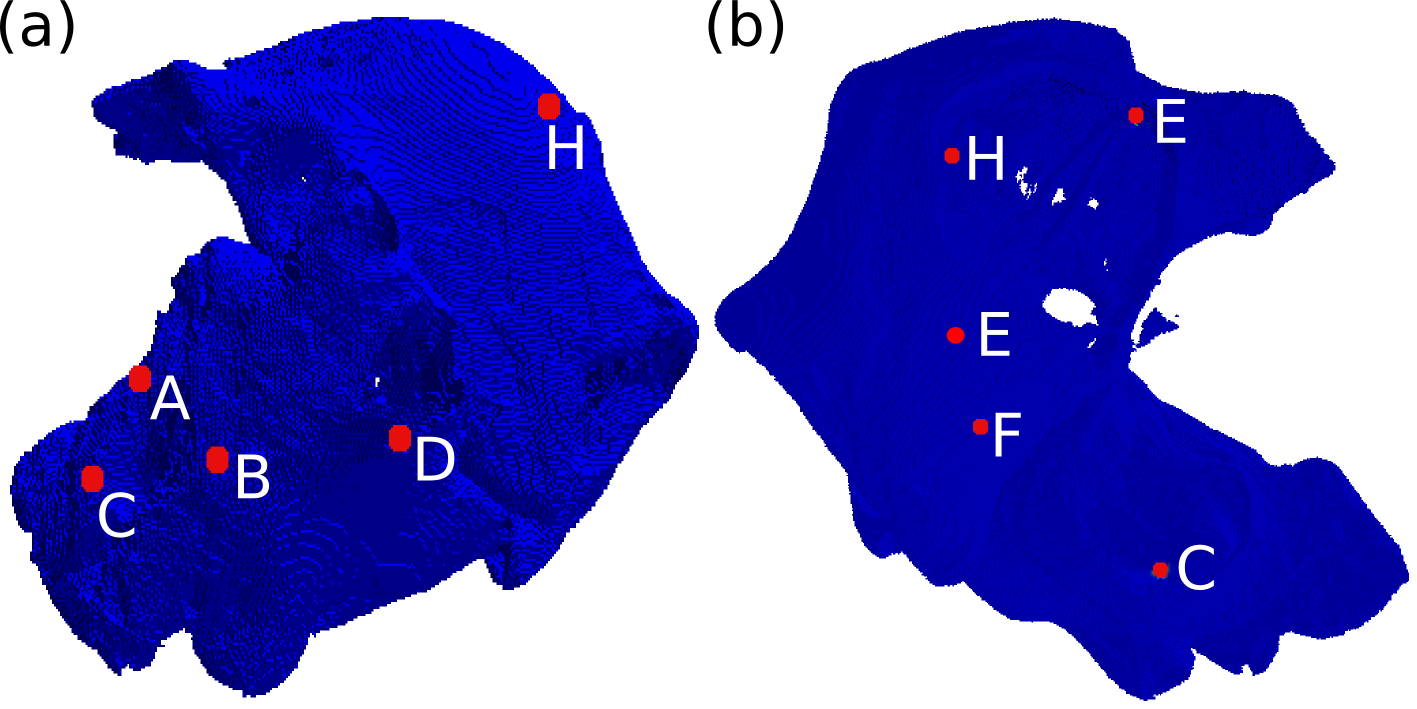
\includegraphics{figures/forward/kistler/pacing_sites}
\end{center}
\caption[Pacing Sites Around The Atria]{
\label{fig:forward:fat:sites}
Pacing sites used assessment of the Kistler~et~al. algorithm.
The pacing centres are indicated by red dots.
Note that sites are often on the interior of the atria at the indicated
locations, or embedded in the wall.

(a) View of the pulmonary veins.
(b) View of up through the valve openings.
}
\end{figure}

\begin{table}
\caption[Pacing Sites Around The Atria]{
\label{tbl:forward:fat:sites}
Anatomical locations of the pacing sites chosen for the study.
Abbreviations: AA = atrial appended, PV = pulmonary vein, TA = tricuspid anulus,
CS = coronary sinus, S = septum, CT = crista terminalis.
L and R denote left and right, respectively.
}
\begin{center}
\begin{tabular}{l l}
\toprule
Site &  Origin \\
\midrule
A & LPV \\
B & LPV \\
C & LPV \\
D & RPV \\
E & RAA \\
F & CS \\
G & LS \\
H & CT \\
\bottomrule
\end{tabular}
\end{center}
\end{table}
\subsection{Results}

\subsubsection{Twelve Lead ECG}

Pacing the atria from different sites results in a dramatic variability in the
observed waveforms of the P-wave ECG.
The ECGs corresponding to the stimuli are shown in
figure~\ref{fig:forward:fat:ecgs}.
The classifications of the waveforms are shown in
table~\ref{tbl:forward:fat:ecgs}.
Classifications consider only the P-wave and not the $\text{T}_{\text{P}}$
wave.
In the case of more than two significant deflections, the largest two are
chosen.
The effect of any electrical flow is exaggerated by the large P-wave magnitudes
previously noted and so it is likely that with correct magnitudes in the
P-waves, these lesser deflections would not show.


\begin{figure}
\begin{center}
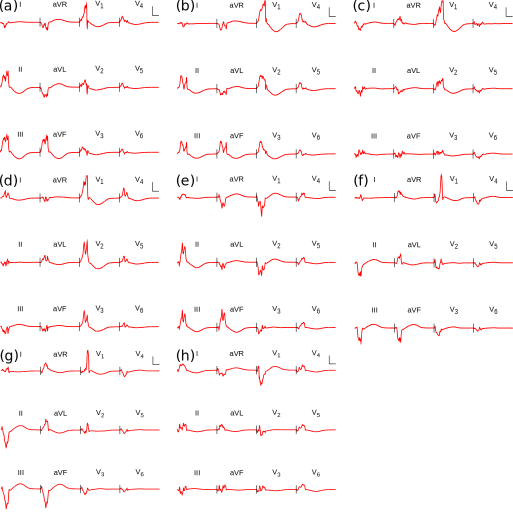
\includegraphics{figures/forward/kistler/ecgs}
\end{center}
\caption[P-wave ECGs For Ectopic Focal Sites]{
\label{fig:forward:fat:ecgs}
Shown is one complete P-wave and $\text{T}_{\text{P}}$ wave, associated with
each of the pacing sites A--H (table~\ref{tbl:forward:fat:sites}).
Scalebars are shown for each figure.
The vertical scale bar is \mv{0.2}, the horizontal \ms{100}.
}

\end{figure}

\begin{table}
\caption[Lead classification from pacing sites through the atria]{
\label{tbl:forward:fat:ecgs}
Lead classification after pacing from sites along the crista terminalis.
Leads are classified based on the criteria used by
Kistler~et~al.~\cite{Kistler2006}.
A positive P-wave is denoted by a $+$ sign, a negative P-wave by a $-$ sign and
a isoelectric (no significant positive or negative component) one by $\sim$.
In the case of a biphasic wave, it is classified based on the polarity of the
two component waves, separated by a slash.
Site denotes the pacing site as illustrated in figure~\ref{fig:forward:fat:sites}.
Site S denotes pacing from the sinus node, and is provided for comparison.
}
\begin{center}
\begin{tabular}{c c c c c c c c c c c c c}
\toprule
Site & I & II & III & aVR & aVL & aVF & $\text{V}_{\text{1}}$ &$\text{V}_{\text{2}}$ & $\text{V}_{\text{3}}$ & $\text{V}_{\text{4}}$ & $\text{V}_{\text{5}}$ & $\text{V}_{\text{6}}$\\
\midrule
S & $+$ & $+$ & $+$ & $-$ & $-$ & $+$ & $+/-$ & $+/-$ & $+$ & $+$ & $+$ & $+$ \\
A & $-$ & $+$ & $+$ & $-$ & $-$ & $+$ & $+/-$ & $+$ & $+$ & $+$ & $+$ & $+$ \\
B & $-$ & $+$ & $+$ & $-$ & $-$ & $+$ & $+$ & $+$ & $+$ & $+$ & $+$ & $+$ \\
C & $\sim$ & $-$ & $\sim$ & $+$ & $\sim$ & $\sim$ & $+$ & $+$ & $+$ & $-$ & $-$ & $-$ \\
D & $+$ & $\sim$ & $-$ & $-$ & $+$ & $-$ & $+$ & $+$ & $+$ & $+$ & $+$ & $+$ \\
E & $+$ & $+$ & $+$ & $-$ & $-$ & $+$ & $-$ & $-$ & $\sim$ & $+$ & $+$ & $+$ \\
F & $+/-$ & $-$ & $-$ & $+$ & $+$ & $-$ & $-/+$ & $-/+$ & $-$ & $-$ & $-$ & $-$ \\
G & $+$ & $-$ & $-$ & $+$ & $+$ & $-$ & $\sim/+$ & $-/+$ & $-$ & $-$ & $-$ & $-$ \\
H & $+$ & $+$ & $-/+$ & $-$ & $+$ & $+$ & $+/-$ & $+/-$ & $+$ & $+$ & $+$ & $+$ \\
\bottomrule
\end{tabular}
\end{center}
\end{table}

Pacing from site A, shown in figure~\ref{fig:forward:fat:ecgs}(a), results in a
P-wave which is positive in most leads.
The P-wave is positive in leads II, III, aVF and $\text{V}_{\text{1--6}}$.
It is negative in leads I, aVR and aVL.
The sharp negative spike visible in $\text{V}_{\text{1, 2}}$ at approximately
\ms{110}\ is caused by the faster conduction along the pectinate muscles, which
are in places disconnected from the main wall of the atrium.
This causes brief high voltage `islands' to appear ahead of the main wavefront,
which generate dipoles of opposing sign to the main wavefront.
This isn't a problem under sinus rhythm, which shows a much more regular
excitation of the pectinate muscles due to the differing origin of excitation.
In addition, the exication wave front has just started to loop back around the
inferior vena cava, travelling away from the frontal precordial leads.
Many of the limb leads show a quite ragged profile, and are slightly bifid.

Pacing from site B, shown in figure~\ref{fig:forward:fat:ecgs}(b), results in a
P-wave which is positive in most leads.
The P-wave is positive in leads II, III, aVF and $\text{V}_{\text{1--6}}$.
It is negative in leads I, aVR and aVL.
All of the inferior leads (II, III and aVF) are smooth but highly bifid.
This occurs as the P-wave depolarises first down the left atrium and then the
right, away from the left limb lead electrode.
After the initial depolarisation of the left atrium from the top and right,
towards the left, much of the excitory activity is parallel to the lateral
precordial leads ($\text{V}_{\text{4--6}}$).

Pacing from site C, shown in figure~\ref{fig:forward:fat:ecgs}(c), results in a
P-wave which is relatively flat.
The P-wave is positive in aVR and $\text{V}_{\text{1--3}}$.
It is negative in leads II and $\text{V}_{\text{4--6}}$.
It is biphasic in leads I, III, aVL, aVF.
The signal in all leads, though especially III, aVF and $\text{V}_{\text{4}}$ is
highly variable.
This is due to an uneven propagating wavefront, caused by the anatomical
obstacles.

Pacing from site D, shown in figure~\ref{fig:forward:fat:ecgs}(d), results in a
P-wave which is mostly positive.
The P-wave is positive in leads I, aVL and $\text{V}_{\text{1--6}}$.
It is clearly bifid in all the leads it is positive in, except lead
$\text{V}_{\text{1}}$.
The P-wave is negative in leads III, aVR and aVF.
It is bifid in both III and aVR.
The ECG is biphasic in lead II.

Site E is shown in figure~\ref{fig:forward:fat:ecgs}(e).
The P-wave is positive in lead I, II, III, AVF and $\text{V}_{\text{5, 6}}$.
The P-wave is negative in lead aVR, aVL and $\text{V}_{\text{1--3}}$.
The P-wave is biphasic in lead $\text{V}_{\text{4}}$.
It is bifid in the positive leads II, III and aVF and in the negative leads aVR,
aVL and $\text{V}_{\text{1, 2}}$.
The P-wave is smooth in most leads, aside from the bifidity.
The electrical excitation is spreading down and slightly to the left of the
body, leading to the very positive potentials observed in the inferior leads,
and the positive potentials in leads $\text{V}_{\text{4--6}}$.
The negative potentials in leads $\text{V}_{\text{1, 2}}$ suggest a spread of
excitation anterior to posterior.

Pacing from site F, figure~\ref{fig:forward:fat:ecgs}(f), produces predominately
negative P-waves.
The P-wave is positive in leads aVR and aVL.
It is negative in leads II, III, aVT and $\text{V}_{\text{3--6}}$.
It is biphasic in leads I, $\text{V}_{\text{1}}$ and $\text{V}_{\text{2}}$.
The P-wave is generally quite clean in all the leads, although it shows
significant oscillation at the end of the P-wave in leads II, III and aVF.
This is likely causes as the excitation wave which is spreading up the right
atrium encounters the complex anisotropy of the junctions between the crista
terminalis and the pectinate muscles.


Pacing from site G, shown in figure~\ref{fig:forward:fat:ecgs}(g), produces a
predominately negative P-wave.
The P-wave is positive in leads I, aVR and aVL.
It is negative in leads II, III, aVF and leads $\text{V}_{\text{3--6}}$.
It is biphasic in leads $\text{V}_{\text{1}}$ and $\text{V}_{\text{2}}$.
The negative leads $\text{V}_{\text{3--6}}$ are indicative of a left atrial
pacing site, with the excitation mostly spreading away from the left.
The positive P-wave in leads aVR and aVL, combined with the negative P-waves in
leads II, III and aVF, suggest the excitation is at the base of the heart and is
spreading upwards.
The lead traces are generally clean.

Site H, figure~\ref{fig:forward:fat:ecgs}(h), produces jagged P-waves.
The P-wave is positive in leads I, II, aVL and $\text{V}_{\text{4--6}}$.
The P-wave is negative in lead aVR.
The P-wave is $-/+$ biphasic in leads III, aVF and $\text{V}_{\text{3}}$.
It is $+/-$ biphasic in leads $\text{V}_{\text{1}}$ and $\text{V}_{\text{2}}$.
Leads II, $\text{V}_{\text{4}}$ and $\text{V}_{\text{5}}$ are bifid.
In addition, leads aVF and $\text{V}_{\text{3}}$ are very bifid in appearance,
although the trough becomes negative enough to classify them as biphasic.

\subsubsection{Application of the Focus Location Algorithm}

The algorithm developed by Kistler~et~al. was applied to the P-wave morphologies
generated by the model.
The algorithm is presented as a simple decision tree, initially concerning the
morphology of lead $\text{V}_{\text{1}}$.
The results of applying the algorithm and the actual anatomical locations are
shown in table~\ref{tbl:forward:fat:kistler}.


\begin{table}
\caption[Classification of focal point tachycardia]{
\label{tbl:forward:fat:kistler}
Classification of the origin of focal point tachycardia according to the
algorithm developed by Kistler~et~al. compared with the actual anatomic
location.
Where the algorithm presents multiple sites as a possibility, both are given.
Abbreviations: AA = atrial appended, PV = pulmonary vein, TA = tricuspid anulus,
CS = coronary sinus, S = septum, CT = crista terminalis.
L and R denote left and right, respectively.
}
\begin{center}
\begin{tabular}{l l l}
\toprule
Site & Predicted  & Origin \\
\midrule
A & CT & LPV \\
B & LAA / LPV & LPV \\
C & RPV & LPV \\
D & RPV & RPV \\
E & RAA / TA & RAA \\
F & CS os / LS & CS \\
G & CS os/ LS & LS \\
H & CT & CT \\
\bottomrule
\end{tabular}
\end{center}
\end{table}

\subsection{Discussion and Conclusion of Focal Atrial Tachycardia Study}

The simulation results show very good agreement with the focal tachycardia
location algorithm developed by Kistler~et~al.
The algorithm, when used on the P-wave ECGs produced by the model, correctly
estimated the origin of the focal point tachycardia in six out of the eight
cases considered.
In addition, one of the errors (case C), is only mistaking between the left and
right pulmonary veins.
This is encouraging as it acts as a validation of both the model and the
algorithm.

The study also highlights some of the limitations of the model.
The most significant of these is the large amplitudes of the P-waves, due to the
nature of the inhomogeneities considered and the underlying cardiac model.
Because of this larger amplitude, several fluctuations that perhaps should be
considered minor are instead classified as full deflections due to the
\mv{0.05}\ threshold.
This is especially evident in case A which is incorrectly classified by the
algorithm as originating from the crista terminalis.
This is due to the presence of the negative spike in lead $\text{V}_{\text{1}}$.
The spike has a magnitude of approximately \mv{0.1} which causes the lead to be
classified as having a positive--negative morphology.
The algorithm classifies all such P-waves as having a crista terminalis origin.
If the spike were of a reduced amplitude, the positive $\text{V}_{\text{1}}$ and
other lead morphologies leads to a classification of LAA or LPV, the correct
answer.

It is also possible that the size of the stimulus zone should be decreased.
The effect of the localised and very rapid potential change along the border of
the stimulus zone can generate a large spike at the start of the pacing cycle.
This is due to the rapid ($ > 200\,\text{mVs}^{\text{-1}}$) upstroke of the
Courtemanche~et~al myocyte model used as the basis of the anatomical atrial
model.
A smaller stimulus zone should reduce this artefact, which is sometimes
difficult to separate from the `real' P-wave.

It should be emphasised, however, that the large amplitudes of the P-wave was
only an issue in case A.
The location of the focal point tachycardia was correctly predicted by the
algorithm in most cases.
This prediction would not be affected by a reduction in amplitude of all the
lead potentials.
The model therefore correctly reproduces the phase information of the P-wave
ECG, which is ultimately what the location algorithm depends on.

The Kistler~et~al. algorithm appears to be the best algorithm one is aware of in
the literature that uses the standard twelve lead ECG.
It would be interesting to compare the predictive accuracy of the algorithm with
one devised using the model and the so called `Atrial ECG' proposed by
Ihara~et~al~\cite{Ihara2007}.
Such a study would require a family of similar models to be developed, based on
several torso and atrial geometrical models.

No discussion of an algorithm of this nature would be complete without a
discussion of inverse techniques.
Inverse techniques have developed considerably over the previous two decades.
Ramanathan~et~al.~\cite{Ramanathan2006}\ have developed a technique which they
call Electrocardiographic Imaging (ECGI) and several groups have similar efforts
as well.
These techniques allow calculation of the epicardial potentials from external
measurements.
These inverse techniques require a significant amount of effort to set up,
however.
The ECGI techinique proposed by Ramanathan~et~al. uses a 224 electrode vest and
requires the construction of a heart--torso geometry from CT scans.
By contrast, algorithms devised for twelve lead sets can still be highly
accurate and are available everywhere.

The Kistler~et~al. model can correctly predict the location of ecotopic foci in
the body surface potential model in seven of eight cases.
This validates both the algorithm and the model.
The model could therefore be used as the basis for further refinements to the
algorithm, or the development of similar ones.

\section{Inverted P-Waves at Night}

Recently an observation was made concerning patients under
24 hour ECG monitoring (Prof. Mark Boyett, Private Conversation, 2008).
It was noted that some patients exhibited inverted P-waves at night.
That is to say, if the patient showed a positive P-wave in leads II and aVF
during the day, then at night the P-wave would be negative in leads II and aVF.
These patients had no known heart disease or conduction defects.
This phenomena has not been reported in the literature.

There is evidence~\cite{Shibata2001,Boineau1988,Dobrzynski2005} that the pacemaker is not a
small and discrete area of the atrium, but is instead distributed along the
length of the crista terminalis.
The presence of certain drugs and hormones, most notably acetylcholine, can cause
the site of the leading pacemaker to move down the pace maker complex.
Acetylcholine is released by what is know as increased `vagal tone'.
This has been observed to happen at night.

The underlying mechanisms for the inverted P-waves at night are unknown.
It was hypothesised that a pacemaker shift induced by increased vagal tone
might lead to the observed P-wave inversion.
In this study, I attempt to verify the hypothesis using the P-wave ECG model.


\subsection{Methods}

In the absence of a model for the distributed pacemaker complex in the human
heart, the direct effects of acetylcholine could not be investigated.
Instead, using the model presented in the previous chapter, several sites were
located along the crista terminalis.
These sites had a radius of 10 nodes (or approximately \mm{3.3}--although this
varied depending on the thickness of the atrial wall at the pacing site), and
therefore were approximately the same size as the sino-atrial node.
These sites are shown in figure~\ref{fig:forward:inverse:ct_sites}.
Each of these sites was stimulated via the same protocol used to stimulate the
sinus node in the original model and then the electrical excitation waves were
allowed to propagate without interference.

\begin{figure}
\begin{center}
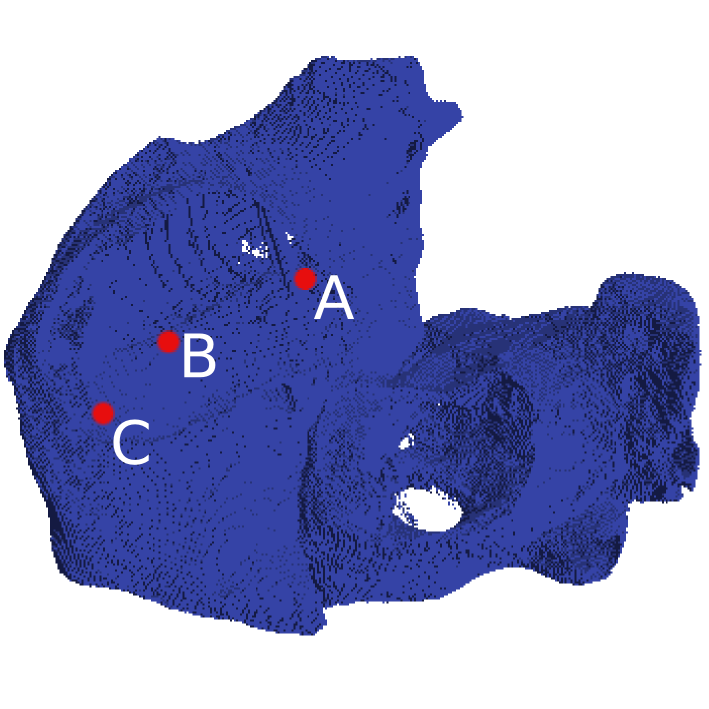
\includegraphics{figures/forward/inverted_p_wave/pacing_sites}
\end{center}
\caption[Pacing Sites Along The CT]{
\label{fig:forward:inverse:ct_sites}
Pacing sites used for the inverted P-wave study.
The view is up through the valve openings.
The pacing centres are indicated by red dots.
}
\end{figure}

The total activation time is calculated as the time after stimulus for all cells
to become excited above \mv{-60}.
ECGs were computed from the patterns of electrical excitation in the atrium.
These were compared to the sinus rhythm ECGs computed in the previous chapter.
In addition, using a so called `inverse Dower' method after Edenbrandt and
Pahlm~\cite{Edenbrandt1988}, the orthogonal components of the ECG were computed
and used to construct representations of the heart
vector~\cite{Frank1956,MacFarlane1989a} ECG (VECG).
To perform the inverse dower transformation, a matrix that has been optimized for
the P-wave (shown in Table~\ref{tbl:forward:idparams}) was
used~\cite{Guillem2007}.


\begin{table}
\caption[Inverse Dower Factors]{
\label{tbl:forward:idparams}
Factors to construct the Frank VECG from the standard 12 lead ECG set.
Parameters optimised to accurately reproduce the P-wave heart
vector~\cite{Guillem2007}.
Each of the 8 leads are multiplied by the given parameters to provide the
orthogonal Frank lead.
}
\begin{center}
\begin{tabular}{c c c c c c c c c}
\toprule
& $\text{V}_{\text{1}}$ &$\text{V}_{\text{2}}$ & $\text{V}_{\text{3}}$ &
$\text{V}_{\text{4}}$ & $\text{V}_{\text{5}}$ & $\text{V}_{\text{6}}$ & I & II \\
\midrule
X & $-0.266$ & $\:0.027$ &  $\:0.065$ & $\:0.131$ & $\:0.203$ & $\:0.220$ & $\:0.370$ & $-0.154$ \\
Y & $\:0.088$ &  $-0.088$ & $\:0.003$ & $\:0.042$ & $\:0.047$ & $\:0.067$ & $-0.131$ & $\:0.717$ \\
Z & $-0.319$ & $-0.198$ & $-0.167$ & $-0.099$ & $\:0.009$ & $\:0.060$ & $\:0.184$ & $\:0.114$ \\
\bottomrule
\end{tabular}
\end{center}
\end{table}

\subsection{Results}

\subsubsection{Activation Sequence}

The activation sequences of the atria after pacing from the sinus node, and the
three sites along the crista terminalis are shown in
figure~\ref{fig:forward:inverse:active}\ as isochronal colour maps.
Time goes from red, at \ms{0}, to blue, at \ms{150}.
The site of first activation obviously shifts depending on the stimulus
location.
In addition, as the stimulus site moves away from the sinus node, the time to
total activation of the atria increases.

\begin{figure}
\begin{center}
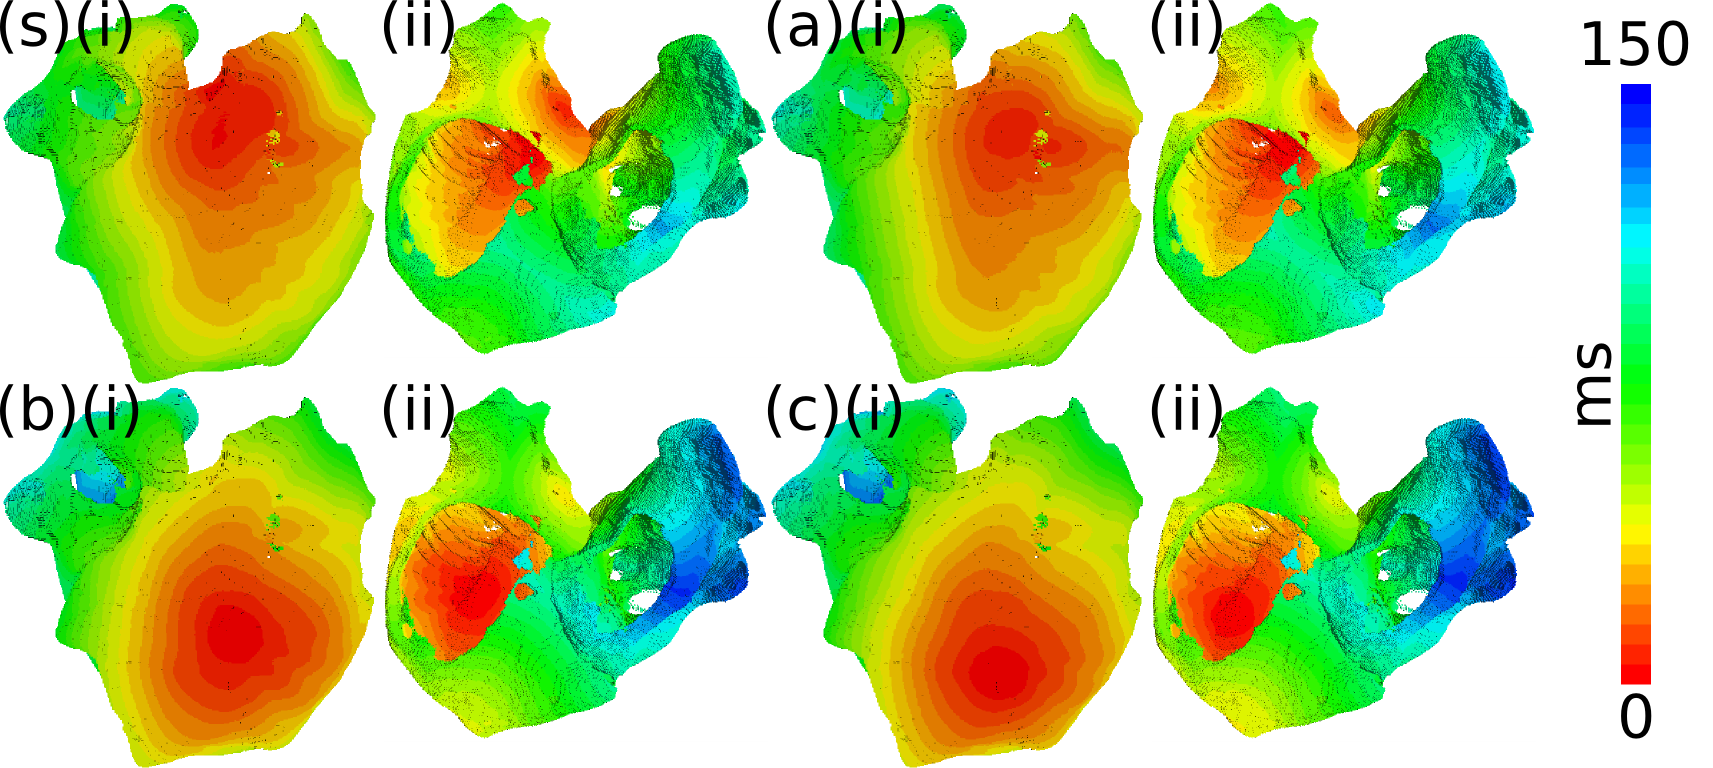
\includegraphics{figures/forward/inverted_p_wave/activation_sequence}
\end{center}
\caption[Activation sequences from pacing sites along the CT]{
\label{fig:forward:inverse:active}
Atrial activation sequences obtained from different pacing sites.
Shown are the activation sequences resulting from pacing at the sinus node, (s),
and the three crista terminalis sites A--C (a--c).
Activation times are represented by colours, going from red at $\leq$\ms{5}\
through green, \ms{75} to deep blue at \ms{150}.
Contours are every \ms{5}.

There are two views shown for each pacing site.
(i), a view of the right atrial surface with the superior vena cava at the top
of the right atrial surface and the tricuspid valve at the base.
In this view, the crista terminalis runs approximately vertically.
(ii), a view up into the atrial cavities through the valve openings.
The ribbed structures of the pectinate muscles are visible through the tricuspid
valve as they extend off the crista terminalis on the left of the panel.
The right and left atrial appendages are to the top of the panels.

In panel (s) the sinus rhythm activation sequence is visible with rapid
conduction along the crista terminalis and pectinate muscles.
The Bachmann's bundle meanwhile rapidly conducts the excitation to the left
atrium.
In both atria, the appendages are amongst the last regions to depolarise.

In panel (a), the activation sequence has shifted slightly down the crista
terminalis.
The pectinate muscles and crista terminalis still have a large influence on the
propagation.
In both atria, the appendages are the last regions to depolarise.

In panel (b), the activation sequence is shifted a long way down the crista
terminalis.
The Bachmann's bundle is no longer the site of first activation of the left
atrium.
Total time to activate is noticeably delayed.

In panel (c), the activation sequence is shifted a long way down the crista
terminalis.
Total time to activate is noticeably delayed in the left atrium.
The Bachmann's bundle is no longer the site of first activation, instead the
area close to the coronary sinus is first activated.
}
\end{figure}

The sinus node activation sequence,
figure~\ref{fig:forward:inverse:active}(s)(i, ii), starts high on the right
atrium, close to the superior vena cava.
Conduction is especially rapid down the crista terminalis and along the
pectinate muscles, visible as the more widely spaced isochrones along these
structures.
The Bachmann bundle, meanwhile, conducts the electrical excitation to the left
atrium, where it then starts to spread over the left atrial endocardial surface.
In the right atrium the activation finishes, approximately \ms{80}\ after
stimulation started, with the activation of the ring around the tricuspid valve
and the right atrial appendage.
In the left atrium, the far extremities of the left atrial appendage and the far
side of the mitral valve to the Bachmann bundle are activated at approximately
\ms{120}, completing the activation of the atria.

The activation sequence from site A,
figure~\ref{fig:forward:inverse:active}(a)(i, ii), starts high on the right
atrium in the region where the pectinate muscles are branching from the crista
terminalis.
This leads to rapid conduction down the pectinate muscles and in both directions
along the crista terminalis.
The Bachmann bundle conducts the excitation to the left atrium, where it starts
to spread.
The activation of the right atrium finishes with the activation of the right
atrial appendage and then region between the septum and the tricuspid valve.
Activation of the left atrium completes in \ms{132}\ after the initial stimulus
on the edge of the left atrial appendage and the mitral valve.

Pacing from site B leads to the activation sequence depicted in
figure~\ref{fig:forward:inverse:active}(b)(i, ii).
The activation sequence starts lower on the crista terminalis, and is conducted
in both directions along the muscle ridge.
The pectinate muscles also influence the conduction, although the excitation
wavefront reaches them later.
Excitation still reaches the left atrium through the Bachmann bundle, although
it is also conducted through the septum close to the inferior vena cava.
The last region to be excited in the right atrium is still the appendage.
In the left atrium, the last activation comes at \ms{140}.
The left atrial appendage and the sheaths of the pulmonary veins both finish
activating at this time.

The activation sequence which results from pacing from site C is shown in
figure~\ref{fig:forward:inverse:active}(c)(i, ii).
The activation sequence starts low on the right atrium and spreads in all
directions, but is faster travelling up the crista terminalis.
The pectinate muscles, when the excitation wave reaches them, also have a
noticeable effect, speeding activation of the right atrium.
Once again, the left atrium appears to be excited in two places, both by the
bachmann's bundle and close to the inferior vena cava through the septum.
The right atrial appendage is the last region of the right atrium to be excited.
In the left atrium, the extremities of the appendage and the pulmonary vein
sheaths are the last to be excited, as well as the region close to the mitral
valve.
The last activation comes at \ms{144}.

All of the activation sequences are approximately normal, in that they travel
from right to left.
The further the stimulus site is removed from the sinus node, the longer
excitation tends to take.


\subsubsection{Twelve Lead ECG}

The ECGs from the three pacing locations along the CT are shown in
figure~\ref{fig:forward:inverse:ecgs}\ with the sinus rhythm P-wave ECG for
comparison.
A summary of the lead deflections for the four cases and sinus rhythm are
presented in table~\ref{tbl:forward:inverse:ecgs}.
There is a clear evolution of the P-wave morphology visible as the pacing site
is moved down the crista terminalis.

\begin{table}
\caption[Lead classification from pacing sites along the CT]{
\label{tbl:forward:inverse:ecgs}
Lead classification of the P-wave after pacing from sites along the crista
terminalis.
Leads are classified based on the criteria used by
Kistler~et~al.~\cite{Kistler2006}.
A positive P-wave is denoted by a $+$ sign, a negative P-wave by a $-$ sign.
In the case of a highly bifid or biphasic wave, the signs of the two phases of
the wave are indicated on either side of a slash.
For example, $+/+$ would be a positive, bifid wave and $-/+$ would be a negative
then positive biphasic wave.
Site denotes the pacing site, where S is the sinus node and Sites A--C are as
indicated in Figure~\ref{fig:forward:ct_sites}.
}
\begin{center}
\begin{tabular}{c c c c c c c c c c c c c}
\toprule
Site & I & II & III & aVR & aVL & aVF & $\text{V}_{\text{1}}$ &$\text{V}_{\text{2}}$ & $\text{V}_{\text{3}}$ & $\text{V}_{\text{4}}$ & $\text{V}_{\text{5}}$ & $\text{V}_{\text{6}}$\\
\midrule
S   & $+$ & $+$ & $+$ & $-$ & $-$ & $+$ & $+/-$ & $+/-$ & $+$ & $+$ & $+$ & $+$ \\
A   & $+$ & $+$ & $+$ & $-$ & $-$ & $+$ & $+/-$ & $-$ & $+$ & $+$ & $+$ & $+$ \\
B   & $+$ & $+/+$ & $-/+$ & $-/-$ & $+$ & $+/+$ & $+/-$ & $+/-$ & $+/+$ & $+/+$ & $+$ & $+$ \\
C   & $+$ & $-/+$ & $-$ & $-$ & $+$ & $-/+$ & $+/-$ & $+/-$ & $-/+$ & $+$ & $+$ & $+$ \\
\bottomrule
\end{tabular}
\end{center}
\end{table}

\begin{figure}
\begin{center}
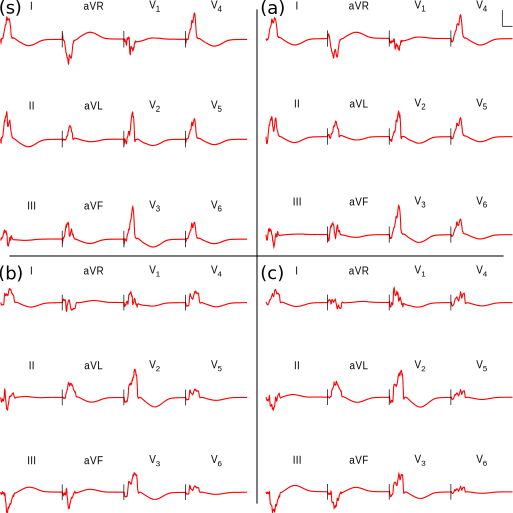
\includegraphics{figures/forward/inverted_p_wave/inverted_pwave_ecg}
\end{center}
\caption[12 Lead ECG traces from pacing sites along the CT]{
\label{fig:forward:inverse:ecgs}
Twelve lead ECG recordings obtained from the model after pacing at the sinus
node, (s) and the three pacing sites A--C (a--c).
Shown is one complete P-wave and $\text{T}_{\text{P}}$ wave, pacing at a rate of
\unit{60}{bpm}.
The scale is the same for all traces, indicated in the top right of panel (a),
where the horizontal scale is in ms and the vertical in mV.
The P-wave is positive in leads II and aVF after pacing from the sinus node.
It is positive in leads II and aVF after pacing from site A.
Pacing from site B leads to a positive but highly bifid P-wave in both leads II
and aVR.
Site C shows negative then positive biphasic P-waves in both leads II and aVR.
}
\end{figure}


The P-wave ECG for pacing from the sinus node,
figure~\ref{fig:forward:inverse:ecgs}(s), is positive in leads II and aVF.
Leads I, III and $\text{V}_{\text{3--6}}$ are also positive.
Leads aVR and aVL are negative.
Leads $\text{V}_{\text{1}}$ and $\text{V}_{\text{2}}$ are both
positive--negative biphasic.
The cardiac axis is between \degr{+60}\ and \degr{+90}\ in the frontal plane.
The ECG is consistent with a normal activation of the atria, spreading to the
left and bottom as time evolves.


Pacing from site A (figure~\ref{fig:forward:inverse:ecgs}(a)), the P-wave ECG is
positive in leads II and  aVF.
Leads I, III,  aVF and $\text{V}_{\text{3--6}}$ are also positive.
Lead aVR, aVL and $\text{V}_{\text{2}}$ are negative
Lead $\text{V}_{\text{1}}$ is posiive--negative biphasic.
The cardiac axis is between \degr{+60}\ and \degr{+90}\ in the frontal plane.
The ECG is consistent with a mostly normal propagation.
The slightly broader negative trough on lead $\text{V}_{\text{1}}$ is due to the
slightly slower depolarisation time of the left atrium.
There is a prominent notch visible in several of the limb leads.
This is caused by the depolarisation of the right atrial appendage and the
pulmonary veins, both of which happen against the bulk direction of excitation
propagation.

Pacing from site B (figure~\ref{fig:forward:inverse:ecgs}(b)), the P-wave ECG
is positive in leads II aVF, but is highly bifid.
Leads I, aVL and $\text{V}_{\text{3--6}}$ are also positive.
Lead aVR is negative.
Lead $\text{V}_{\text{1}}$ and $\text{V}_{\text{2}}$ are positive--negative
biphasic.
Lead III is negative--positive biphasic.
The cardiac axis is approximately \degr{+30} in the frontal plane.
The bifid morphology of the P-wave in the inferior limb leads and aVR is due to
the delayed depolarisation of the left atrium, induced by the time taken to
propagate up the crista terminalis.
The bidirectional propagation contributes to the much lower amplitudes observed
in many of the limb leads compared to the sinus rhythm.


Pacing from site C (figure~\ref{fig:forward:inverse:ecgs}(c)), the P-wave ECG is
negative--positive biphasic in leads II and aVR.
Leads I, aVL and $\text{V}_{\text{4--6}}$ are positive.
Leads III and aVR are negative.
Lead $\text{V}_{\text{1}}$ and $\text{V}_{\text{2}}$ are positive--negative
biphasic.
Lead $\text{V}_{\text{3}}$ is negative--positive.
biphasic.
The cardiac axis is approximately $0^\circ$ in the frontal plane, as the
excitation wave now travels mostly across the atria.
The negative--positive morphology of the P-wave in leads II and aVR are caused
as the bulk direction of the excitation is first up the right atrium and then
down the left atrium.
The lateral precordial leads ($\text{V}_{\text{4--6}}$) are positive as the
excitation is still travelling from right to left.

As the pacing site moves down the crista terminalis there is an evolution of the
P-wave, which is visible in all leads.
As a result of the shift, the cardiac axis shifts through about $90^\circ$
anti-clockwise from the sinus direction of $+90^\circ$.
The P-wave duration increases slightly as the crista terminalis increases,
highlighting the importance of the specialized conduction structures of the
heart in rapidly conducting the excitation wave.


\subsubsection{Derived Vector ECGs}

\begin{figure}
\begin{center}
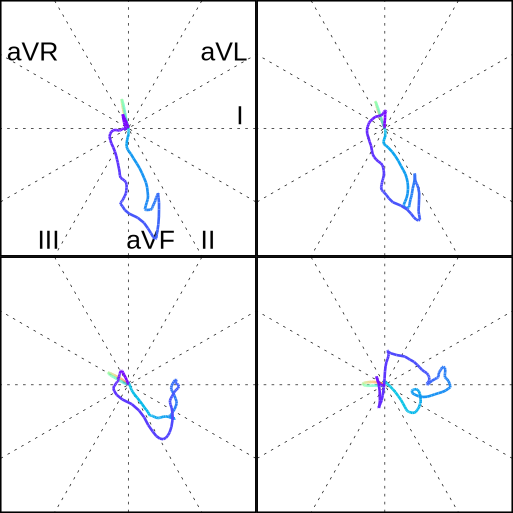
\includegraphics{figures/forward/inverted_p_wave/frontal_vector_loops}
\end{center}
\caption[Frontal plane vector loops from pacing sites along the CT]{
\label{fig:forward:inverse:vec_front}
Frontal plane vector loops, constructed from the derived vECG for pacing at the
sinus node, (s) and the three pacing sites A--C (a--c).
Shown is one complete P-wave and $\text{T}_{\text{P}}$ wave, pacing at a rate of
\unit{60}{bpm}.
Colour represents the passage of time, going from purple (\ms{0}) through blue
(\ms{250}) to red (\ms{500}) after the initiation of the stimulus.
The horizontal and vertical scales are centred at \mv{0}\ in the centre of the
figure and extending out to $\pm$\mv{0.4}.}
\end{figure}

\begin{figure}
\begin{center}
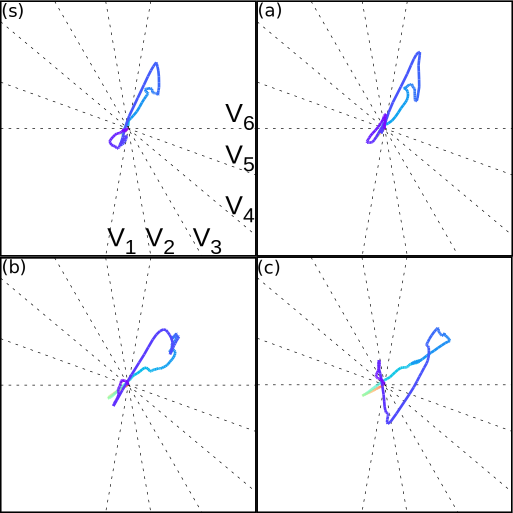
\includegraphics{figures/forward/inverted_p_wave/transverse_vector_loops}
\end{center}
\caption[Transverse plane vector loops from pacing sites along the CT]{
\label{fig:forward:inverse:vec_trans}
Transverse plane vector loops, constructed from the derived vECG for pacing at the
sinus node, (s) and the three pacing sites A--C (a--c).
Shown is one complete P-wave and $\text{T}_{\text{P}}$ wave, pacing at a rate of
\unit{60}{bpm}.
Colour represents the passage of time, going from purple (\ms{0}) through blue
(\ms{250}) to red (\ms{500}) after the initiation of the stimulus.
The horizontal and vertical scales are centred at \mv{0}\ in the centre of the
figure and extending out to $\pm$\mv{0.4}.}
\end{figure}

The derived vector ECG plots are shown for the frontal plane in
figure~\ref{fig:forward:inverse:vec_front} and in the transverse plane in
figure~\ref{fig:forward:inverse:vec_trans}.
Again, the sinus rhythm is included in both figures for reference.
The colour of the vector loop represents the passage of time and is coloured
from purple, at \ms{0}, through blue, green, yellow and ending up red at
\ms{500} after initiation of the P-wave.

The vector loop in the frontal plane for sinus rhythm is shown in
figure~\ref{fig:forward:inverse:vec_front}(s).
The vector loop is inscribed in an anti-clockwise direction.
The efferent, or outgoing, limb is at approximately \degr{+90}, before it loops up to its
maximal extension at approximately \degr{+75}.
The afferent, or incoming, limb is at approximately \degr{+70}.
The $\text{T}_{\text{P}}$ wave is visible as a small anti-clockwise loop,
almost linear, aligned at approximately \degr{-100}.
The initial deflection along almost the same line is an artefact of the stimulus
protocol.
The P-wave loop is open, although like the ECGs it is not entirely smooth.

The frontal plane vector loop for pacing from site A,
figure~\ref{fig:forward:inverse:vec_front}(a), is inscribed in an anti-clockwise
direction.
The loop is generally open, although there is a noticeable direction change
where the afferent limb briefly returns to the efferent limb.
This corresponds to the notch visible in the inferior limb leads.
The main axis of the loop is at approximately \degr{+70}.
The efferent limb is aligned at approximately \degr{+60}, along the line of lead
II.
The $\text{T}_{\text{P}}$ wave is visible as a small loop, aligned at
approximately \degr{-120}.

Pacing from site B produces the frontal plane vector loop in
figure~\ref{fig:forward:inverse:vec_front}(b).
The loop is largely inscribed in an anticlockwise direction.
The main axis of the loop is aligned at approximately \degr{+40}.
The efferent limb is relatively smooth as it travels out along an approximately
\degr{+60}\ vector.
The loop then sweeps up to \degr{+0}, crossing over itself several times, before
it returns smoothly to 0.
The $\text{T}_{\text{P}}$ is a small clockwise loop at an angle of \degr{-120}.
The loop from site C has the smallest area of the loops.

The frontal plane vector loop from pacing at site C is shown in
figure~\ref{fig:forward:inverse:vec_front}(c).
The loop is largely inscribed in as a very uneven figure-of-eight which is
initially anticlockwise and is then clockwise.
The main axis of the loop is aligned at approximately \degr{+0}.
The efferent limb is initially at \degr{+90}\ before it doubles back on itself
to sweep up at an angle of \degr{-90}.
It then sweeps down to \degr{+0}, and the point of maximal extension.
The afferent limb then sweeps back, inscribing a minor clockwise loops.
The $\text{T}_{\text{P}}$ is a small anticlockwise loop at an angle of \degr{-180}.

As the pacing site moves down the crista terminalis there are clear changes in
the morphology and principle axis of the P-wave frontal vector loop.
The axis shift which could be determined from the 12 lead ECG was clearly
highlighted.
The vector loops also show the reduction in amplitude of the P-wave as the
pacing location is moved down the crista terminalis, possibly caused by the
generally slower speed of activation.
The $\text{T}_{\text{P}}$ wave axis is opposite the main axis of the loop in all
cases.

In contrast to the frontal plane vector plots, the transverse plane plots bear
much less resemblance to the associated leads ($\text{V}_{\text{1--6}}$).
The differences manifest in both the magnitude and the direction.
This makes it hard to directly compare the transverse plane vector plots with
the cardiac activity.
The loops generated appear to be too flat and too negative in the Z (vertical)
direction, which is especially obvious in the sinus rhythm plot
(\ref{fig:forward:inverse:vec_trans}(s)).

\subsection{Discussion and Conclusions of Inverted P-wave Study}

As the stimulus site moves down the crista terminalis the patterns of electrical
activation in the atrium change noticeably.
The focal point of excitation obviously moves down the crista terminalis to
follow this.
It is also interesting to note the similarities.
Despite the shifting activation site, the right atrial appendage and the region
between the tricuspid valve and the atrial septum are always the last to
activate in the right atrium.
In the left atrium, the appendage also activates last in all cases.

As the pacing site moves away from the sinus node, the total activation time
increases.
However, total activation times remain within those observed clinically by
Lemery~et~al.~\cite{Lemery2004}\ for all three pacing locations away from the
sinus node.
The activation patterns are similar to those observed by
Boineau~et~al.~\cite{Boineau1988}\ as the pacing location moves, although the
Boineau data does not include single activations away from the sinus node.

The latter two sites (B \& C), which are low on the crista terminalis, appear to
reach the left atrium in part through a site which emerges close to the coronary
sinus~\cite{Platonov2007,Platonov2008,Markides2003,Lemery2004}.
There is no specialist inferior intra-atrial conduction pathway in the model
however.
Conduction along this lower route is therefore at the normal bulk tissue rate.
It is possible if this were treated specially in the model total activation
times would be reduced.

The ECGs generated from the model also show an evolution as the stimulus site
moves down the crista terminalis.
This change is more visible in the limb leads than in the precordial leads.
This is to be expected, as the propagation remained from right to left in all
cases, but whether it is travelling up or down the atria changes as the pacing
site does.
The P-waves in leads II and aVF is positive in during sinus rhythm, and both
gradually invert as the pacing site shifts down the crista terminalis, as
hypothesised.

As the pacing site moves away from the sinus node, the P-wave duration also
increases.
Especially for the lower crista terminalis sites (B \& C), the duration exceeds
normal P-wave limits~\cite{Lemery2004,MacFarlane1989}.
It is possible that a more detailed intra-atrial conduction system, including an
inferior pathway would reduce total conduction time, and therefore P-wave
duration in these cases.

The P-wave vector loops are similar to those observed in clinical
studies~\cite{Carlson2005,Holmqvist2007,Havmoller2007,Guillem2008}, although the typical
presentation of such loops as monochromatic does make comparison of the timing
information and direction of inscription hard.
They make it quite obvious that the cardiac axis shifts as the pacing location
does.
The morphology of the loops can be used to gain further clues, such as with the
initial rise and then fall visible in the Site B frontal vector loops.

The limitations of the body surface potential model have been discussed
previously ($\S$\ref{sec:bsp:limits}).
Of particular importance to this study is the lack of a distributed sinus node
model~\cite{Yamamoto2007,Dobrzynski2005}\ for the human atrium.
However, pacemaker shift under the influence of
acetylcholine~\cite{Shibata2001}\ has been observed in rabbits and in
humans~\cite{Opthof1988}\ so it seems plausible as a mechanism for the shifts
and associated P-wave inversions.
The use of an inverse dower matrix to obtain the frank leads rather than
directly measuring them was chosen to allow more direct comparison with clinical
data, which is often only for the standard twelve leads.
The selection of the correct transform matrix is
important~\cite{Guillem2008,Luo1991b,Hyttinen1995}\ and it is possible that the
vector loop accuracy could be improved by the use of a transformation matrix
optimised for the body surface potential model~\cite{vanOosterom2007}.
This is especially true for the Z-axis, which has the lowest correllation
coefficient of the leads~\cite{Hyttinen1995}.
Alternatively a true frank lead system, or a hybrid model could be constructed.

The hypothesis that P-wave inversion could be caused by pacemaker shift in the
human sinus node seems to be plausible.
Progressive shift of the pacemaker site down the sinus node leads to progressive
inversion of the observed P-waves in leads II and aVF.
In addition, this shift is accompanied by other changes which do not stray too
far from normality.
This is important, as the shift was originally observed in those with no
diagnosed cardiac disorders.
Further investigation is merited, once an appropriate model of the distributed
sino-atrial node complex can be integrated into the atrial model.

This study shows that the body surface potential model can be used for a study
which involves conditions that begin to deviate from normality.
It can therefore be used as a powerful tool for investigating the clinically
observable consequences of changes to cardiac behaviour.

\section{Discussion and Conclusion}

The constructed model has been used in two separate studies.
The first was a validation of an existing clinically derived algorithm for
predicting the origin of focal point tachycardia.
The second study concerned itself with investigation into a new clinical
phenomena, that of inverted P-waves at night.


The focal tachycardia algorithm study confirms the performance of the algorithm.
This validates both the algorithm and the model.
The study also highlights a potential weakness in the model, that of the high
amplitudes it produces.
Despite this problem, the model still performs well and was `well behaved'
according to the algorithm under test.
In addition, there is no indication that a reduction in the amplitude due to a
more complete consideration of the inhomogeneities would adversely impact this.

The inverted P-wave study confirms that a suggested mechanism for inverted
P-waves at night, that of pacemaker shift under increased vagal tone, is
plausible.
The ECGs calculated by the model show a clear evolution as the pacing site
shifts further down the crista terminalis.
Additional validation is is obviously required with a suitable model of a
distributed pacemaker complex.

The model developed is therefore a useful tool for cardiac modelling.
It can enhance the conclusions that can be drawn from 3D simulations with
further clinical relevance.


   \chapter{Discussion And Conclusions}


This was an investigation into models of cardiac tissue, with a special focus on
atrial tissue.
It included whole atrial models, which were then extended beyond the heart to
simulate the P-wave ECG.
A toolkit providing access to efficient implementations of various experimental
protocols was developed.
A model of the atrium based on biophysically detailed myocyte models, including tissue heterogeneity and anisotropic
conduction, was constructed.
The atrial model was used as the basis of a model of the P-wave ECG which was
solved using a boundary elemental formulation.
All of the tools and models developed were used to perform physiological
studies of tissues in healthy and diseased states.

\section{Cardiac Simulation Toolkit}

The cardiac toolkit which was developed provides easy access to a wide variety
of experimental protocols.
These protocols are used to assess the physiological impact of a gene mutation,
drug action, hormonal effect or other electrophysiological modification.
They include protocols which act on single cells and also on one dimensional
idealisations of cardiac tissue.

The implementations of these protocols focused on efficient algorithms
which take advantage of the computational nature of the models.
It was important that this did not compromise on the physiological accuracy and
level of detail employed.
This was accomplished in part through the use of lookup tables which reduced the
computational effort needed to solve \ms{1}\ of cardiac activity compared to an
implementation without such tables without impacting measured physiological
characteristics significantly.
Such a saving might be considered a `cell level' performance optimisation.
Greater savings can be observed through the use of `protocol level' performance
optimisation.
These protocol level optimisations are where the computational nature of the
models can really be exploited.
Optimisations include storing of cellular state after the pre-pacing part of the
protocol and adaptive stepping when tracking response curves of varying slope.
There was also the novel use of a basic computer science algorithm, the binary
search, to determine the limits in a number of experimental protocols.
This can be used, with a sensible choice of initial guesses, to reduce the total
number of cases which must be tested by an order of magnitude.

The toolkit also offers an easy way of specifying and running 2D simulations.
Simulation, even of irregular geometry, is simplified.
Utilities can be used to convert quantified colour bitmaps into simulation
geometries with heterogeneous electrophysiology.
A variety of stimulation protocols can be specified, including both current and
voltage stimuli.
The simulations are accompanied by regular outputting of gif snapshots of the
voltage, to allow simulations to be assessed as they run.
In addition, the tissue simulation code is parallelized using a shared memory
paradigm with OpenMP.

\section{Whole Atrial Model}

The whole atrium model which was developed is capable of modeling the
electrophysiological behaviour of the atrium at the whole tissue level.
It includes both conduction anisotropy and tissue heterogeneity.
The use of biophysically detailed myocyte model as the basis makes the model
flexible.
Diffusion of voltage was altered to produce conduction velocities in the atrial
tissue comparable with those measured experimentally and to reproduce clinical
measurement of total activation time under sinus rhythm.
The model is based on an anatomical geometry, not an idealised one, including
fluctuations in wall thickness and other anatomical deviations.
All these features make the model suitable for modeling a variety of conditions.
This includes those induced by fundamental changes to the electrophysiology
caused by genetic defects or drug actions.

The level of detail might make the model computationally unattractive, as it
involves solving many ordinary differential equations to advance the cellular
state as well as calculating the diffusion between many cells.
The model is parallelized, using a shared memory paradigm, allowing the effort
to be split over several cores.
The biophysically detailed model used as the basis uses precomputed lookup
tables to calculate many of the parameters which influence the gating variables,
reducing repetition of effort at minimal cost of overall accuracy.
Repeated calculations are also reduced by pre-computation of the Laplacian
operator used to diffuse the voltage.
This is especially useful in the relatively thin walled atria, which therefore
have many more boundary cells.
All these refinements keep the total computational time within acceptable limits
whilst maintaining the biophysical detail required for many studies.

Using the toolkit and a simplified version of the whole atrial model the
effects of a novel gene mutation, the S140G mutation in the KCNQ1 gene, were
assessed.
This gene has been linked to the prevalence of atrial fibrillation in a Chinese
family afflicted with it.
The gene affects the \ii{Ks}\ channel, adding an instantaneous component to the
channel kinetics.
This additional leakage component dramatically abbreviates the action potential
duration. 
The restitution curves of the model were flattened and lowered by the influence of the
mutation, reducing the rate response of the tissue.
This allowed the tissue to sustain pacing at very high rates
($>$\unit{500}{bpm}) which were observed clinically.
Simulations in a two-dimensional tissue model revealed that the spatial
vulnerability window was reduced, suggesting that a much smaller region of
ectopic activity would be needed to incite arrhythmic activity.
The two dimensional models also suggested that the mutation allowed longer
lived spiral waves to exist in the tissue which would form a stable mother
rotor.
Simulations using the atrium model suggested that whilst in normal tissue
arrhythmic excitation would often decay away, in tissues afflicted with the
S140G mutation sustained arrhythmic activity was observed.
This activity was often a sustained mother rotor, but sometimes the anatomical
features present in the atrial model could lead to breakup into complex,
fibrilatory activity.

\section{Body Surface Potential Model}

A model of the P-wave body surface potential using the boundary element method
was created.
This used the atrial model as the basis for calculating the cardiac dipoles.
The meshes representing the body and selected internal inhomogeneities were
based on CT scans although they had been simplified considerably.
The atrium was located within the mesh using the internal inhomogeneities as
guides as well as anatomical descriptions of the location of the atria.
From the computed body surface potential traces were extracted to represent the
12 lead ECG and body surface potential maps.


Again, computational tractability was an important concern.
This motivated the choice to use the boundary element method.
In addition, the dipole contributions of several nodes of the atrial model were
aggregated together and assumed to act at the centroid of the aggregated region.
This reduced the total number of dipole sources by three orders of magnitude,
whilst having negligible impact on the final result.
The meshes were refined for the final computations to produce high quality body
surface potential maps.
This had almost no influence on the computed ECGs suggesting that for ECG
centric studies, such a refined mesh was not required.
Even with the refined mesh the problem remained tractable, solving \unit{1}{s}\
of body surface potential calculations in an acceptable time using only one
core.
The implementation itself is quite flexible, allowing for easy incorporation of
further meshes representing more internal detail.

Using the model the influence of internal inhomogeneities was examined.
It was found that the lungs tended to amplify the magnitudes of signals seen in
the leads, whilst the presence of blood masses tended to reduce them.
The inhomogeneities had little influence on the phase of the signals observed in
the 12 lead ECG, which showed good agreement with the clinical norms of the
P-wave ECG.
The amplitudes of the signal, in contrast, tended to be outside the normal
physiological range.
The reason for this was not entirely clear.
It could be due to the lack of consideration of certain inhomogeneities, such as
the skeletal bones or the skeletal muscle layer.
It might also be possible that a better model of the bloodmasses would reduce
this.

Despite the high amplitudes observed the model is still useful.
The phase relationships are generally of more interest clinically as are the
relative, rather than the absolute, amplitudes.
Because of the biophysically detailed basis of the atrial model, the body
surface potential model can be used in a variety of physiological studies to
provide insight into the clinically observable effects of the studied influence.

\section{Applications of the Body Surface Potential Model}

The body surface potential model was used to investigate two cases of clinical
interest.
It was used to assess an algorithm developed by physicians for locating the
origin of focal point tachycardia.
Also, a novel clinical phenomena, inverted P-waves at night, was investigated.

Focal atrial tachycardia is a supraventricular tachycardia characterised by
excitation emerging from an ectopic focus site.
It is readily treated by radio ablation therapy which is aided by accurate
knowledge of the focal site.
The algorithm presented used a decision tree approach, based on the waveform of
several 12 lead ECG leads.
To assess the algorithm, the model was paced from several ectopic sites around
the atria.
The ECG was used to make a decision based on the algorithm and this was compared
to the actual origin.
The origins predicted by the algorithm were in good agreement to the real pacing
locations in 6 out of 8 cases and showed only minor difference (left verses
right pulmonary veins) in one further case.
The final case, which is quite inaccurate, would probably be resolved were the
amplitudes closer to the clinically observed ranges--or if the algorithm's
threshold were adjusted to account for the higher potentials.
The good agreement provides validation of both the focal point origin algorithm
and the model itself.

Inverted P-waves at night are a phenomena which has not been reported on in the
literature.
They have been observed in the inferior limb leads in certain cases in patients
undergoing 24 hour cardiac monitoring.
It was hypothesised that this could be due to pacemaker shift in a distributed
pacemaker complex, induced by hormonal changes at night.
To investigate this hypothesis, the body surface potential model was paced from
several sites along the crista terminalis, to represent progressively greater
degree of shift and then the twelve lead ECG was computed.
It was observed that as the pacing site moved further along the crista
terminalis, the P-wave ECG in the inferior leads flattened and then inverted, in
accordance with the hypothesis.
Pacemaker shift is therefore a viable mechanism for the observed P-wave changes
at night.

\section{Future Work}

The work presented here opens up many paths for future efforts.
The models and tools developed in the study can be refined.
They can also be used, with and without such refinement, for new studies.

The toolkit developed can be extended in a number of ways.
The library of cellular models available can be increased, either through
direct addition, or by the development of a converter which can take CellML
models and produce code suitable for use.
More experimental protocols could be added to the toolkit, expanding its
utility.
The use of more sophisticated integrators for cellular equations could be
incorporated into the models and their influence on the performance and results
assessed.
The toolkit could also be expanded into three dimensions, allowing the same ease
of specifying numerical experiments to be enjoyed in whole heart simulations.

The atrial model can also be refined in a number of ways.
As new models of atrial tissue are developed, they can be incorporated into the
model so that it always represents the best knowledge we have of the atrium and
its complexities.
A more complete map of the regions and directions of preferential conduction
could be incorporated into the model which could be important for non-sinus
rhythm cases.
For some studies an accurate and auto-active pacemaker complex would be a
benefit.
Contraction, and the associated mechanical and electric coupling, could be
incorporated into the model.

Beyond the atrium, the body surface model has several avenues for further study.
The influence of further inhomogeneities can be investigated.
Patient specific studies, where the cardiac geometry and torso structure are
based on CT and MRI scans of the patient offer exciting possibilities.
First, direct comparison with clinical data allows for further validation of the
underlying model.
Such models can also be used to suggest and test appropriate clinical
procedures.

Patient specific models also allow for the possibility of developing a family of models,
representing different orientations and conformations of the atrium and the
surrounding torso.
Using such a family of models would allow the results of computational studies
to be stated with more confidence.
An effect observed in one model might be an artefact of the geometry, but an
affect observed in five or ten or more is much less likely to be so.

Without any refinement, the toolkit and models developed offer a good basis for
many electrophysiological studies on a variety of scales.
The biophysical detail employed makes them suitable for the investigation of
complex effects.
The computational efficiency makes relatively long term simulations a
possibility too.


%    \bibliography{refs}
    \bibliography{refs_full}

\end{document}
